% ============================================================
%  THE MIDNIGHT BREWER
%  Building a contactless payment terminal from scratch
%
%  Build:  latexmk -pdf brewer-book.tex
%  (or:    pdflatex brewer-book && makeindex brewer-book && pdflatex x2)
% ============================================================
\documentclass[11pt,twoside,openright]{book}

% ============================================================
%  The Midnight Brewer -- preamble / design system
%  Compile with: pdflatex (or latexmk -pdf)
% ============================================================

\usepackage[T1]{fontenc}
\usepackage[utf8]{inputenc}

% ---- fonts -------------------------------------------------
\usepackage[mono=false]{libertinus}      % body serif
\usepackage[scaled=0.92]{FiraSans}       % headings sans
\usepackage[scaled=0.86]{sourcecodepro}  % code mono
\usepackage{microtype}

% ---- page geometry -----------------------------------------
\usepackage[
  paperwidth=7.5in, paperheight=9.25in,
  inner=0.95in, outer=0.85in,
  top=0.95in, bottom=1.0in,
  headsep=18pt, footskip=28pt
]{geometry}

\usepackage{graphicx}
\usepackage{amssymb}      % \square for checklists
\usepackage{booktabs}
\usepackage{array}
\usepackage{longtable}
\usepackage{multirow}
\usepackage{enumitem}
\usepackage{xcolor}
\usepackage{tikz}
\usetikzlibrary{positioning,arrows.meta,calc,shapes.geometric,fit,backgrounds,decorations.pathreplacing}
\usepackage[most]{tcolorbox}
\usepackage{listings}
\usepackage{fancyhdr}
\usepackage{titlesec}
\usepackage{makeidx}
\usepackage{emptypage}
\usepackage[bottom]{footmisc}

\usepackage[
  colorlinks=true,
  linkcolor=brewerlink,
  urlcolor=brewerlink,
  citecolor=brewerlink,
  pdftitle={The Midnight Brewer},
  pdfsubject={Building a contactless payment terminal from scratch},
  pdfauthor={Martin},
  bookmarksnumbered=true
]{hyperref}

\makeindex

% ---- palette -----------------------------------------------
\definecolor{brewerink}   {HTML}{16161D}  % near-black body
\definecolor{brewernavy}  {HTML}{1B2A4A}  % headings
\definecolor{brewerlink}  {HTML}{1F5C99}
\definecolor{breweramber} {HTML}{B26B00}  % analogy
\definecolor{brewerred}   {HTML}{A32C2C}  % traps
\definecolor{brewergreen} {HTML}{1F6B4A}  % verification
\definecolor{brewerblue}  {HTML}{27548A}  % concepts
\definecolor{brewergrey}  {HTML}{5A5F6B}
\definecolor{rulegrey}    {HTML}{C9CCD2}
\definecolor{codebg}      {HTML}{F7F7F9}
\definecolor{codeframe}   {HTML}{DDDFE4}
\definecolor{kwcolor}     {HTML}{7A3E9D}
\definecolor{strcolor}    {HTML}{1F6B4A}
\definecolor{comcolor}    {HTML}{6B7280}
\definecolor{todocolor}   {HTML}{B26B00}

\color{brewerink}

% ---- headings ----------------------------------------------
\titleformat{\part}[display]
  {\normalfont\sffamily\bfseries\color{brewernavy}}
  {\Large\MakeUppercase{Part \thepart}}{14pt}{\Huge}
\titleformat{\chapter}[display]
  {\normalfont\sffamily\bfseries\color{brewernavy}}
  {\normalsize\sffamily\mdseries\color{brewergrey}\MakeUppercase{Chapter \thechapter}}
  {8pt}{\LARGE\raggedright}
  [\vspace{4pt}{\color{rulegrey}\rule{\linewidth}{0.6pt}}]
\titleformat{\section}
  {\normalfont\sffamily\bfseries\large\color{brewernavy}}{\thesection}{0.7em}{}
\titleformat{\subsection}
  {\normalfont\sffamily\bfseries\normalsize\color{brewernavy}}{\thesubsection}{0.6em}{}
\titlespacing*{\chapter}{0pt}{6pt}{22pt}
\titlespacing*{\section}{0pt}{18pt}{6pt}
\titlespacing*{\subsection}{0pt}{13pt}{4pt}

% ---- running heads -----------------------------------------
\pagestyle{fancy}
\fancyhf{}
\renewcommand{\headrulewidth}{0.4pt}
\renewcommand{\headrule}{\hbox to\headwidth{\color{rulegrey}\leaders\hrule height \headrulewidth\hfill}}
\fancyhead[LE]{\sffamily\small\color{brewergrey}\leftmark}
\fancyhead[RO]{\sffamily\small\color{brewergrey}\rightmark}
\fancyfoot[C]{\sffamily\small\color{brewergrey}\thepage}
\renewcommand{\chaptermark}[1]{\markboth{\textsc{The Midnight Brewer}}{}}
\renewcommand{\sectionmark}[1]{\markright{#1}}
\fancypagestyle{plain}{\fancyhf{}\renewcommand{\headrulewidth}{0pt}%
  \fancyfoot[C]{\sffamily\small\color{brewergrey}\thepage}}

% ---- code listings -----------------------------------------
\lstdefinestyle{brewerbase}{
  basicstyle=\ttfamily\footnotesize,
  backgroundcolor=\color{codebg},
  frame=single,
  rulecolor=\color{codeframe},
  framesep=6pt,
  xleftmargin=10pt, xrightmargin=0pt,
  breaklines=true,
  breakatwhitespace=false,
  breakindent=14pt,
  postbreak=\mbox{\textcolor{brewergrey}{$\hookrightarrow$}\space},
  columns=fullflexible,
  keepspaces=true,
  showstringspaces=false,
  tabsize=4,
  upquote=true,
  aboveskip=10pt, belowskip=8pt,
  keywordstyle=\color{kwcolor}\bfseries,
  commentstyle=\color{comcolor}\itshape,
  stringstyle=\color{strcolor},
  numberstyle=\tiny\color{brewergrey},
  literate=%
    {á}{{\'a}}1 {é}{{\'e}}1 {í}{{\'i}}1 {ó}{{\'o}}1 {ú}{{\'u}}1
    {€}{{\texteuro}}1 {—}{{---}}1 {–}{{--}}1 {'}{{'}}1
    {“}{{``}}1 {”}{{''}}1 {…}{{\ldots}}1 {×}{{$\times$}}1
    {⚠}{{!}}1 {→}{{$\rightarrow$}}1 {‖}{{$\|$}}1 {≥}{{$\geq$}}1
}

\lstdefinestyle{java}{style=brewerbase,language=Java,
  morekeywords={var,record,sealed,permits,yield},
  moredelim=[il][\color{todocolor}\bfseries]{//!},
}
\lstdefinestyle{dart}{style=brewerbase,language=Java,
  morekeywords={Future,async,await,final,var,late,Uint8List,int,void,class,extends},
}
\lstdefinestyle{bash}{style=brewerbase,language=bash,
  keywordstyle=\color{brewernavy}\bfseries,
}
\lstdefinestyle{xml}{style=brewerbase,language=XML,
  morestring=[b]",
}
\lstdefinestyle{plain}{style=brewerbase,
  keywordstyle=\color{brewerink},
  basicstyle=\ttfamily\scriptsize,
}

\lstset{style=java}

% shorthand environments
\lstnewenvironment{jcode}[1][]{\lstset{style=java,#1}}{}
\lstnewenvironment{dcode}[1][]{\lstset{style=dart,#1}}{}
\lstnewenvironment{shell}[1][]{\lstset{style=bash,#1}}{}
\lstnewenvironment{xcode}[1][]{\lstset{style=xml,#1}}{}
\lstnewenvironment{trace}[1][]{\lstset{style=plain,#1}}{}

% inline code
\newcommand{\code}[1]{\texttt{\small #1}}
\newcommand{\hex}[1]{\texttt{\small #1}}
\newcommand{\reg}[1]{\textsf{\small #1}}

% ---- callout boxes -----------------------------------------
\newtcolorbox{analogybox}[1][]{
  enhanced, breakable,
  colback=breweramber!5, colframe=breweramber,
  borderline west={2.6pt}{0pt}{breweramber},
  frame hidden, arc=0pt, outer arc=0pt,
  boxrule=0pt, left=10pt, right=10pt, top=8pt, bottom=8pt,
  fonttitle=\sffamily\bfseries\small\color{breweramber},
  title={ANALOGY}, attach title to upper={\par\vspace{3pt}},
  #1
}

\newtcolorbox{trapbox}[1][]{
  enhanced, breakable,
  colback=brewerred!4, colframe=brewerred,
  borderline west={2.6pt}{0pt}{brewerred},
  frame hidden, arc=0pt, outer arc=0pt,
  boxrule=0pt, left=10pt, right=10pt, top=8pt, bottom=8pt,
  fonttitle=\sffamily\bfseries\small\color{brewerred},
  title={TRAP}, attach title to upper={\par\vspace{3pt}},
  #1
}

\newtcolorbox{conceptbox}[1][]{
  enhanced, breakable,
  colback=brewerblue!5, colframe=brewerblue,
  borderline west={2.6pt}{0pt}{brewerblue},
  frame hidden, arc=0pt, outer arc=0pt,
  boxrule=0pt, left=10pt, right=10pt, top=8pt, bottom=8pt,
  fonttitle=\sffamily\bfseries\small\color{brewerblue},
  title={CONCEPT}, attach title to upper={\par\vspace{3pt}},
  #1
}

\newtcolorbox{verifybox}[1][]{
  enhanced, breakable,
  colback=brewergreen!5, colframe=brewergreen,
  borderline west={2.6pt}{0pt}{brewergreen},
  frame hidden, arc=0pt, outer arc=0pt,
  boxrule=0pt, left=10pt, right=10pt, top=8pt, bottom=8pt,
  fonttitle=\sffamily\bfseries\small\color{brewergreen},
  title={VERIFICATION GATE}, attach title to upper={\par\vspace{3pt}},
  #1
}

\newtcolorbox{deepbox}[1][]{
  enhanced, breakable,
  colback=black!3, colframe=brewergrey,
  borderline west={2.6pt}{0pt}{brewergrey},
  frame hidden, arc=0pt, outer arc=0pt,
  boxrule=0pt, left=10pt, right=10pt, top=8pt, bottom=8pt,
  fonttitle=\sffamily\bfseries\small\color{brewergrey},
  title={GOING DEEPER}, attach title to upper={\par\vspace{3pt}},
  #1
}

% titled variants
\newtcolorbox{analogy}[1]{enhanced,breakable,colback=breweramber!5,
  borderline west={2.6pt}{0pt}{breweramber},frame hidden,arc=0pt,boxrule=0pt,
  left=10pt,right=10pt,top=8pt,bottom=8pt,
  title={\sffamily\bfseries\small\color{breweramber}ANALOGY\quad#1},
  attach title to upper={\par\vspace{3pt}},colframe=breweramber}
\newtcolorbox{trap}[1]{enhanced,breakable,colback=brewerred!4,
  borderline west={2.6pt}{0pt}{brewerred},frame hidden,arc=0pt,boxrule=0pt,
  left=10pt,right=10pt,top=8pt,bottom=8pt,
  title={\sffamily\bfseries\small\color{brewerred}TRAP\quad#1},
  attach title to upper={\par\vspace{3pt}},colframe=brewerred}
\newtcolorbox{concept}[1]{enhanced,breakable,colback=brewerblue!5,
  borderline west={2.6pt}{0pt}{brewerblue},frame hidden,arc=0pt,boxrule=0pt,
  left=10pt,right=10pt,top=8pt,bottom=8pt,
  title={\sffamily\bfseries\small\color{brewerblue}CONCEPT\quad#1},
  attach title to upper={\par\vspace{3pt}},colframe=brewerblue}
\newtcolorbox{deeper}[1]{enhanced,breakable,colback=black!3,
  borderline west={2.6pt}{0pt}{brewergrey},frame hidden,arc=0pt,boxrule=0pt,
  left=10pt,right=10pt,top=8pt,bottom=8pt,
  title={\sffamily\bfseries\small\color{brewergrey}GOING DEEPER\quad#1},
  attach title to upper={\par\vspace{3pt}},colframe=brewergrey}

% ---- chapter opener block ----------------------------------
% \chapterbrief{goal}{concept}{you end with}
\newcommand{\chapterbrief}[3]{%
  \begin{tcolorbox}[enhanced, colback=brewernavy!4, colframe=brewernavy!25,
    arc=2pt, boxrule=0.5pt, left=12pt, right=12pt, top=10pt, bottom=10pt,
    before skip=2pt, after skip=18pt]
    \setlength{\parskip}{4pt}
    {\sffamily\bfseries\footnotesize\color{brewernavy}GOAL}\quad #1\par
    {\sffamily\bfseries\footnotesize\color{brewernavy}CONCEPT}\quad #2\par
    {\sffamily\bfseries\footnotesize\color{brewernavy}YOU END WITH}\quad #3
  \end{tcolorbox}}

% ---- misc --------------------------------------------------
\setlist[itemize]{leftmargin=1.35em, itemsep=2pt, topsep=4pt}
\setlist[enumerate]{leftmargin=1.6em, itemsep=2pt, topsep=4pt}
\renewcommand{\arraystretch}{1.22}
\setlength{\parskip}{0.45em}
\setlength{\parindent}{0pt}
\setcounter{secnumdepth}{2}
\setcounter{tocdepth}{1}

% table helpers
\newcolumntype{L}[1]{>{\raggedright\arraybackslash}p{#1}}
\newcommand{\thead}[1]{\textsf{\bfseries\small #1}}

% a "symptom / cause" trap table
\newenvironment{traptable}{%
  \par\vspace{4pt}
  \small
  \begin{longtable}{L{0.42\linewidth} L{0.52\linewidth}}
  \toprule \thead{You see} & \thead{Cause / fix} \\ \midrule
  \endhead
}{%
  \bottomrule
  \end{longtable}
  \normalsize
}


\begin{document}

% ============================================================
\frontmatter
% ============================================================

% ---------- title page ----------
\begin{titlepage}
\thispagestyle{empty}
\centering
\vspace*{0.55in}

{\sffamily\fontsize{15}{18}\selectfont\color{brewergrey}
 THE\quad MIDNIGHT\quad BREWER\par}

\vspace{0.42in}
{\color{brewernavy}\rule{3.1in}{1.1pt}}\par
\vspace{0.30in}

{\sffamily\bfseries\fontsize{31}{36}\selectfont\color{brewernavy}
 Building a Contactless\\[3pt] Payment Terminal\\[3pt] From Scratch\par}

\vspace{0.28in}
{\color{brewernavy}\rule{3.1in}{1.1pt}}\par
\vspace{0.34in}

{\fontsize{13}{18}\selectfont\itshape
 From SPI bytes to AES mutual authentication ---\\
 every layer written by hand, on a \pounds3 reader\\ and a Raspberry Pi.\par}

\vspace{0.50in}

% --- a small card-tap vignette ---
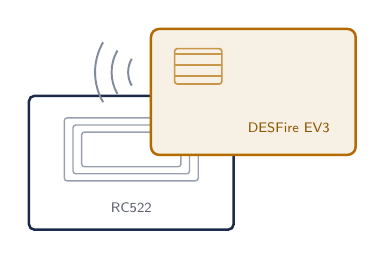
\begin{tikzpicture}[scale=1.0]
  % reader
  \draw[rounded corners=2pt, brewernavy, line width=0.9pt]
        (0,0) rectangle (2.6,1.7);
  \node[font=\sffamily\tiny, color=brewergrey] at (1.3,0.28) {RC522};
  % antenna coil
  \foreach \i in {0,1,2}{
    \draw[brewernavy!45, line width=0.5pt, rounded corners=1pt]
      (0.45+0.11*\i,0.62+0.09*\i) rectangle (2.15-0.11*\i,1.42-0.09*\i);
  }
  % card
  \draw[rounded corners=3pt, draw=breweramber, fill=breweramber!10, line width=0.9pt]
        (1.55,0.95) rectangle (4.15,2.55);
  \draw[breweramber!70, line width=0.6pt, rounded corners=1pt]
        (1.85,1.85) rectangle (2.45,2.3);
  \foreach \y in {1.95,2.09,2.23}{ \draw[breweramber!70, line width=0.5pt] (1.85,\y)--(2.45,\y); }
  \node[font=\sffamily\tiny, color=breweramber!80!black] at (3.3,1.3) {DESFire EV3};
  % waves
  \foreach \r in {0.34,0.55,0.76}{
    \draw[brewernavy!55, line width=0.7pt] (1.6,2.0) ++(150:\r) arc (150:210:\r);
  }
\end{tikzpicture}

\vfill
{\sffamily\small\color{brewergrey}
 A build-it-yourself book\quad$\cdot$\quad Java\;$\cdot$\;Dart\;$\cdot$\;C-to-OOP\par}
\vspace{6pt}
{\sffamily\footnotesize\color{brewergrey} Revision \today\par}
\end{titlepage}

\cleardoublepage

% ---------- colophon ----------
\thispagestyle{empty}
\vspace*{\fill}
{\small
\textbf{The Midnight Brewer: Building a Contactless Payment Terminal From Scratch}\par
\vspace{8pt}
A companion to the \code{DesfireVendingMachine} project. Every implementation
described here exists, runs on a Raspberry Pi Zero~2~W with a \pounds3 MFRC522
module, and debits a real MIFARE DESFire EV3 card.\par
\vspace{10pt}
\textbf{On the code in this book.} The listings are deliberately incomplete.
They give you the class shape, the constants and the byte layouts, and leave
the logic as \code{TODO}. That is the method, not an oversight --- see
\emph{How to use this book} on page~\pageref{sec:howtouse}.\par
\vspace{10pt}
\textbf{Safety.} Chapter~\ref{ch:android} describes commands that can
\emph{permanently} destroy a contactless card. Use dedicated test cards.
Never run provisioning against a card you did not buy for this project.\par
\vspace{10pt}
\textbf{Security.} The keys printed in this book are bench keys, published
here on purpose. They protect nothing. Section~\ref{sec:realkeys} explains what
a real deployment does instead.\par
}
\vspace*{\fill}

\cleardoublepage
\tableofcontents

\cleardoublepage
\chapter*{Preface}
\addcontentsline{toc}{chapter}{Preface}
\markboth{\textsc{Preface}}{}

There is a moment, somewhere around the middle of this book, when a small
plastic card and a three-pound circuit board prove to each other that they both
know the same sixteen-byte number --- without either of them ever transmitting
it, and while anyone within a few centimetres could be recording every bit that
passes between them.

That moment is the reason this book exists. It is the same handshake that
happens when you tap your bank card, open your office door, or board a train.
It is not magic and it is not beyond you. It is about two hundred lines of code,
and by the end of Chapter~\ref{ch:auth} you will have written all of them.

\section*{What you will build}

A coffee kiosk that takes contactless payments. Touch a drink on a
touchscreen, hold a card to the reader, and:

\begin{enumerate}
  \item the reader wakes the card out of the radio field and reads its serial number;
  \item your code and the card authenticate each other with AES-128;
  \item your code reads the balance --- encrypted, and authenticated, so a
        forged reply is rejected rather than believed;
  \item it debits the price, commits the transaction, and the drink is dispensed.
\end{enumerate}

Plus a phone app that puts credit back on.

Every layer is yours. No NFC library, no crypto library beyond a raw AES block
cipher, no copied driver. You will write the SPI register encoding, the
anticollision tree walk, the ISO-DEP block framing, AES-CMAC from the RFC, the
session key derivation, the mutual authentication, and the secure messaging that
carries the money.

\section*{Who this is for}

You know C. You have blinked an LED, read a datasheet, and written
\code{uint8\_t buf[16]}. You have probably not written much Java, and you may
never have seen an interface, an abstract class, or a line of cryptography.

That is exactly the intended reader. This book teaches object-oriented design
and applied cryptography \emph{as tools for a job you are actually doing}, in the
order the job demands them.

\begin{concept}{No concept before the problem that needs it}
You will not read ``an interface is a contract between a class and its
callers'' as an abstract definition. You will hit a concrete wall --- \emph{I
cannot test my driver without a Raspberry Pi physically plugged in} --- and the
interface will be the tool that gets you over it.

Concepts learned that way stick, because they are attached to a memory of being
stuck. Concepts learned as definitions evaporate before the exam.
\end{concept}

Each chapter names the one design idea it introduces:

\begin{center}\small
\begin{tabular}{@{}ll@{}}
\toprule
\thead{Chapter} & \thead{Idea, and the problem that forces it} \\
\midrule
1  & Interfaces --- testing a driver with no hardware \\
2  & Encapsulation --- forty copies of a bit-twiddle \\
3  & Abstract classes --- one protocol, many reader chips \\
4  & Polymorphism --- three frame types, one call site \\
5  & Value objects --- three results that belong together \\
6  & Layering --- a seam that makes crypto testable \\
7  & Immutability --- an object that cannot be half-built \\
8  & Enums over booleans --- \code{derive(key, a, b, true)} means nothing \\
9  & Injecting randomness --- testing a function that is random \\
10 & Growing a class --- state and its operations belong together \\
11 & The Adapter pattern --- two fixed interfaces, made to fit \\
12 & Porting a design --- discovering what was incidental \\
\bottomrule
\end{tabular}
\end{center}

\section*{How to use this book}
\label{sec:howtouse}

\textbf{Read the chapter, close the book, write the code.} Every chapter gives
you five things:

\begin{enumerate}
  \item \textbf{The problem.} What does not work yet, concretely.
  \item \textbf{The idea.} The design, with an analogy from outside programming.
  \item \textbf{The boilerplate.} A skeleton with \code{TODO} comments.
  \item \textbf{The verification gate.} A test with known-good values.
        \emph{Do not continue until it passes.}
  \item \textbf{The traps.} The specific bugs that will bite, with their symptoms.
\end{enumerate}

\subsection*{Why the listings have holes in them}

Because reading code teaches you very little and writing it teaches you almost
everything.

The skeletons hand you the parts that are pure lookup --- register addresses,
class declarations, import lists, byte layouts --- and withhold the parts that
are actual reasoning: the algorithm, the control flow, the order of operations.
You spend your thinking where thinking pays.

If you get genuinely stuck, a complete implementation of every file exists in
the companion repository. Treat it as the back of a textbook: consulting it ends
the exercise, so spend twenty minutes stuck first. \emph{Being stuck is the
learning.} The answer merely ends it.

\subsection*{The verification gate, and why it is not optional}

Cryptographic code has a property that no code you have written before has:
\textbf{wrong output is indistinguishable from right output.}

A broken checksum gives you a visible mismatch. A broken CMAC gives you sixteen
bytes of perfect-looking randomness --- exactly like a correct CMAC. You cannot
eyeball it. You cannot infer it from a failed transaction. And if you build three
more layers before testing, you will have no way to know which one is lying.

On real hardware it is worse: a card may count consecutive authentication
failures and, after enough of them, lock a key permanently.

So every chapter in Part~IV ends with \textbf{known-answer test vectors} ---
inputs with independently computed correct outputs. Reproduce them and your code
is right. Fail them and it is wrong, and you fix it \emph{now}.

The vectors in this book were generated with Python's \code{cryptography}
library, deliberately \emph{not} with the Java you are writing. Otherwise they
would only prove your code agrees with itself.

\section*{What you need}

\begin{center}\small
\begin{tabular}{@{}L{0.34\linewidth}L{0.46\linewidth}r@{}}
\toprule
\thead{Item} & \thead{Notes} & \thead{Approx.} \\
\midrule
Raspberry Pi Zero 2 W & Any Pi works; the Zero 2 W is the tight fit that teaches you to optimise & \pounds18 \\
MFRC522 reader module & The ubiquitous breakout board & \pounds3 \\
\textbf{MIFARE DESFire EV2/EV3} & \textbf{Not Classic, not NTAG. See below.} & \pounds3 ea \\
7-inch touchscreen \emph{(optional)} & 1024$\times$600, HDMI + USB touch & \pounds45 \\
Jumper wires, microSD, 5\,V PSU & & \\
An Android phone with NFC & For Part~VI & \\
\bottomrule
\end{tabular}
\end{center}

\begin{trap}{The card matters more than anything else on that list}
It must say \textbf{DESFire EV2} or \textbf{EV3}. Not MIFARE Classic (broken
crypto, entirely different protocol), not NTAG or Ultralight (no crypto at all,
no value files), not ``13.56\,MHz RFID tag'' from a bag of a hundred.

If a listing says ``compatible'' or does not name the chip, it is not one.
\textbf{Buy at least two} --- one to develop against and one spare, because it
is genuinely possible to destroy a card by changing a key and forgetting it.

You can confirm what you have in Chapter~\ref{ch:apdu}: a real DESFire answers
\code{GetVersion} with a hardware type byte of \hex{0x33} for EV3.
\end{trap}

\section*{Conventions}

\begin{itemize}
  \item Java 21 and Maven, package \code{com.midnightbrewer}. Keeping the same
        package as the reference repository means you can diff against it.
  \item Hexadecimal is lowercase and unspaced in code, spaced in prose:
        \hex{91 00}.
  \item Coloured rules in the margin mark the four kinds of aside:
        \textcolor{brewerblue}{concepts}, \textcolor{breweramber}{analogies},
        \textcolor{brewerred}{traps}, and \textcolor{brewergreen}{verification
        gates}.
  \item Every chapter ends with a suggested commit message, so your history
        becomes a record of the build.
\end{itemize}

\vspace{1em}
\begin{flushright}
\itshape One layer at a time.
\end{flushright}


% ============================================================
\mainmatter
% ============================================================

\part{Groundwork}
\chapter{Setup: hardware, Pi, and an empty project}
\label{ch:setup}

\chapterbrief
  {An RC522 wired to a Pi, a Java project that compiles, and one green test.}
  {None yet --- this chapter removes every excuse the environment can give you later.}
  {\code{mvn compile} passing, and a chip you can talk to.}

Nothing in this chapter is interesting, and that is the point. Every hour spent
later wondering \emph{``is this my code or my wiring?''} is an hour you can buy
back now by making the environment boring and trustworthy.

\section{Wiring the RC522}
\index{RC522!wiring}\index{SPI!wiring}

The RC522 speaks SPI: six signal wires plus power.

\begin{center}\small
\begin{tabular}{@{}llll@{}}
\toprule
\thead{RC522 pin} & \thead{Pi pin} & \thead{Pi name} & \thead{Why} \\
\midrule
\reg{3.3V} & 1  & 3V3            & \textbf{Never 5\,V.} The MFRC522 is a 3.3\,V part. \\
\reg{RST}  & 22 & BCM 25         & Hardware reset \\
\reg{GND}  & 6  & GND            & \\
\reg{MISO} & 21 & BCM 9 (MISO)   & Chip $\rightarrow$ Pi \\
\reg{MOSI} & 19 & BCM 10 (MOSI)  & Pi $\rightarrow$ chip \\
\reg{SCK}  & 23 & BCM 11 (SCLK)  & Clock \\
\reg{SDA}  & 24 & BCM 8 (CE0)    & Chip select --- confusingly labelled with an I\textsuperscript{2}C name \\
\reg{IRQ}  & --- & not connected & We poll instead; simpler, and fast enough \\
\bottomrule
\end{tabular}
\end{center}

\begin{center}
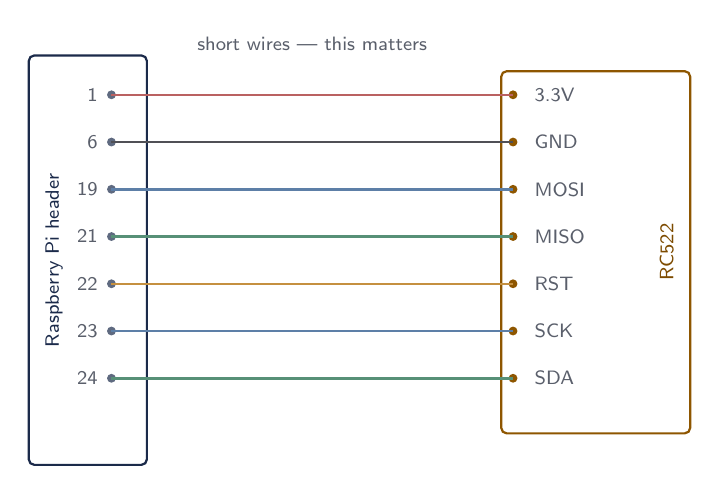
\begin{tikzpicture}[
   pin/.style={font=\scriptsize\sffamily},
   wire/.style={line width=0.9pt},
   x=1cm,y=1cm]

  % Pi header
  \draw[rounded corners=2pt, brewernavy, line width=0.8pt] (0,0) rectangle (1.5,5.2);
  \node[pin, color=brewernavy, rotate=90] at (0.32,2.6) {Raspberry Pi header};
  \foreach \y/\lbl in {4.7/1, 4.1/6, 3.5/19, 2.9/21, 2.3/22, 1.7/23, 1.1/24}{
     \fill[brewernavy!70] (1.05,\y) circle (1.6pt);
     \node[pin, color=brewergrey, anchor=east] at (1.0,\y) {\lbl};
  }

  % RC522
  \draw[rounded corners=2pt, breweramber!80!black, line width=0.8pt] (6.0,0.4) rectangle (8.4,5.0);
  \node[pin, color=breweramber!70!black, rotate=90] at (8.1,2.7) {RC522};
  \foreach \y/\lbl in {4.7/3.3V, 4.1/GND, 3.5/MOSI, 2.9/MISO, 2.3/RST, 1.7/SCK, 1.1/SDA}{
     \fill[breweramber!80!black] (6.15,\y) circle (1.6pt);
     \node[pin, color=brewergrey, anchor=west] at (6.3,\y) {\lbl};
  }

  % wires
  \foreach \y/\c in {4.7/brewerred, 4.1/brewerink, 3.5/brewerblue,
                     2.9/brewergreen, 2.3/breweramber, 1.7/brewerblue, 1.1/brewergreen}{
     \draw[wire, color=\c!75] (1.05,\y) -- (6.15,\y);
  }
  \node[pin, color=brewergrey] at (3.6,5.35) {short wires --- this matters};
\end{tikzpicture}
\end{center}

\begin{trap}{Long wires are not a style question}
At 1\,MHz over 20\,cm of loose DuPont jumper you get intermittent failures that
look exactly like firmware bugs: a version register that reads \hex{0x00} on one
run and \hex{0x92} on the next.

If the chip is flaky, \textbf{shorten the wires before you debug a single line
of code}. More people have lost an evening to this than to any bug in this book.
\end{trap}

\section{Pi OS and SPI}

Flash Raspberry Pi OS (64-bit), then enable SPI:

\begin{shell}
sudo raspi-config       # Interface Options -> SPI -> Enable
sudo reboot
ls -l /dev/spidev0.0    # must exist after the reboot
\end{shell}

\code{/dev/spidev0.0} is the kernel exposing ``SPI bus 0, chip-select 0'' as a
file. That file is the entire hardware interface: everything in Part~II is
ultimately reads and writes to it.

Add your user to the hardware groups, or Pi4J cannot open the device:

\begin{shell}
sudo usermod -aG spi,gpio $USER    # log out and back in
sudo apt update
sudo apt install -y openjdk-21-jdk maven
java -version                      # expect 21.x
\end{shell}

\section{Create the project}

Develop on a laptop and deploy to the Pi. Compiling on a Zero 2 W is slow
enough to break your concentration.

\begin{shell}
mkdir midnight-brewer && cd midnight-brewer
git init
mkdir -p src/main/java/com/midnightbrewer/hardware
mkdir -p src/test/java/com/midnightbrewer/hardware
\end{shell}

\subsection{The \texttt{pom.xml}}

Maven's project file. Three things matter: Java 21, JUnit 5, and Pi4J.

\begin{xcode}
<project xmlns="http://maven.apache.org/POM/4.0.0">
  <modelVersion>4.0.0</modelVersion>
  <groupId>com.midnightbrewer</groupId>
  <artifactId>MidnightBrewer</artifactId>
  <version>1.0-SNAPSHOT</version>

  <properties>
    <maven.compiler.source>21</maven.compiler.source>
    <maven.compiler.target>21</maven.compiler.target>
    <project.build.sourceEncoding>UTF-8</project.build.sourceEncoding>
    <pi4j.version>3.0.2</pi4j.version>
  </properties>

  <dependencies>
    <!-- Pi4J: Java access to the Pi's SPI and GPIO -->
    <dependency>
      <groupId>com.pi4j</groupId><artifactId>pi4j-core</artifactId>
      <version>${pi4j.version}</version>
    </dependency>
    <!-- the SPI provider: talks to /dev/spidev0.0 -->
    <dependency>
      <groupId>com.pi4j</groupId><artifactId>pi4j-plugin-linuxfs</artifactId>
      <version>${pi4j.version}</version>
    </dependency>
    <!-- the GPIO provider, for the reset pin -->
    <dependency>
      <groupId>com.pi4j</groupId><artifactId>pi4j-plugin-gpiod</artifactId>
      <version>${pi4j.version}</version>
    </dependency>
    <!-- Pi4J logs through SLF4J; without a binding it prints warnings -->
    <dependency>
      <groupId>org.slf4j</groupId><artifactId>slf4j-simple</artifactId>
      <version>2.0.13</version>
    </dependency>

    <dependency>
      <groupId>org.junit.jupiter</groupId><artifactId>junit-jupiter</artifactId>
      <version>5.10.2</version>
      <scope>test</scope>
    </dependency>
  </dependencies>

  <build><plugins>
    <plugin>
      <groupId>org.apache.maven.plugins</groupId>
      <artifactId>maven-surefire-plugin</artifactId>
      <version>3.2.5</version>
    </plugin>
  </plugins></build>
</project>
\end{xcode}

\begin{concept}{\texttt{<scope>test</scope>} is a boundary, not a detail}
It means ``this library exists when compiling and running tests, but is not
shipped with the application.'' Get it wrong and your kiosk drags a test
framework onto the Pi.

More usefully, it \emph{enforces} the boundary: if you accidentally
\code{import org.junit} in main code, the build fails. A dependency scope is the
build system letting you state a design rule and have it checked.
\end{concept}

\begin{shell}
mvn -q compile     # should print nothing and exit 0
\end{shell}

There is nothing to compile yet. You have proven that Maven, Java and the
network can all do their jobs --- which is exactly one fewer thing that can be
wrong tomorrow.

\section{Java for a C programmer}
\index{Java!versus C}

You will meet the rest as you go, but four things trip up every C programmer on
the first day.

\subsection{Every function lives inside a class}

There are no free functions. \code{Math.abs()} is a function \code{abs} inside a
class \code{Math}. A file \code{Foo.java} contains \code{class Foo}. This feels
bureaucratic, and for small programs it is --- but it is also why the language
can make guarantees C cannot, and Part~II is where those guarantees start paying
for themselves.

\subsection{\texttt{byte} is signed, and there is no \texttt{unsigned}}
\index{signed byte}

This will bite you within the hour.

\begin{jcode}
byte b = (byte) 0x92;
System.out.println(b);          // -110   <-- the same bits, read as signed
System.out.println(b & 0xFF);   // 146    <-- what you meant
\end{jcode}

\hex{0x92} is \code{1001 0010}. With the top bit set, Java reads it as negative.
The fix is the idiom \code{\& 0xFF}, which promotes to \code{int} and masks off
the sign extension.

\begin{trap}{The \texttt{\& 0xFF} habit}
\textbf{Any time you turn a \code{byte} into a number, write \code{\& 0xFF}.}
You will forget this at least once and lose an hour to a register that reads
$-110$ instead of \hex{0x92}. Everyone does. Now you have been warned, and you
will still do it.
\end{trap}

\subsection{Arrays know their own length, and are bounds-checked}

\code{arr.length} --- no parentheses, it is a field. Reading past the end throws
an exception naming the line, rather than silently returning whatever was next in
memory. This converts C's worst class of bug into a stack trace.

\subsection{No manual memory management}

No \code{malloc}, no \code{free}. \code{new byte[16]} gives you sixteen
\emph{zeroed} bytes, and they vanish when nothing refers to them. The zeroing
matters more than you would think: several structures in this book are ``a
16-byte buffer that is mostly zeros'', and you get that for free.

\medskip
One C habit transfers perfectly: bit manipulation. \code{<<}, \code{>>},
\code{\&}, \code{|}, \code{\^{}} and \code{\~{}} all mean exactly what they mean
in C. The register-poking half of this project will feel like home.

\section{Commit}

\begin{shell}
git add -A
git commit -m "chore: empty Maven project, Java 21, Pi4J + JUnit"
\end{shell}


\part{Talking to the Chip}
\chapter{The SPI seam}
\label{ch:spi}

\chapterbrief
  {Define what ``an SPI bus'' means to your program, build a fake one, and test against it with no hardware attached.}
  {Interfaces, and dependency injection.}
  {A green test that runs with the reader unplugged.}

\section{The problem}

You are about to write a driver that pokes RC522 registers. Before you write a
line of it, ask an uncomfortable question:

\begin{quote}\itshape How will I know the driver is correct?\end{quote}

The obvious answer --- \emph{plug in the Pi and see} --- will cost you the
project. Consider the loop it commits you to:

\begin{center}
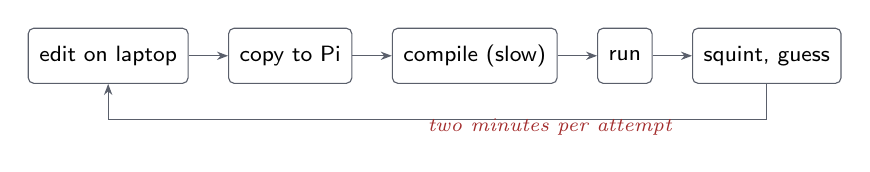
\begin{tikzpicture}[node distance=5mm, font=\footnotesize\sffamily,
   b/.style={draw=brewergrey, rounded corners=2pt, inner sep=4pt, minimum height=7mm}]
  \node[b] (e) {edit on laptop};
  \node[b, right=of e] (c) {copy to Pi};
  \node[b, right=of c] (m) {compile (slow)};
  \node[b, right=of m] (r) {run};
  \node[b, right=of r] (g) {squint, guess};
  \foreach \x/\y in {e/c, c/m, m/r, r/g}{
    \draw[-{Stealth[length=4pt]}, brewergrey] (\x) -- (\y);}
  \draw[-{Stealth[length=4pt]}, brewergrey] (g.south) -- ++(0,-4.5mm) -| (e.south);
  \node[font=\scriptsize\itshape, color=brewerred] at ($(m)!0.5!(r)+(0,-9mm)$)
       {two minutes per attempt};
\end{tikzpicture}
\end{center}

And every failure has three possible causes --- your logic, your wiring, the
chip --- with no way to tell them apart. You want a loop that takes 200
milliseconds and has exactly \emph{one} possible cause: your logic.

\section{The idea: program against a description, not a thing}

Your driver does not actually need ``a Raspberry Pi SPI bus''. Look at what it
truly needs: \emph{something that takes bytes out and hands bytes back}. That is
the entire requirement. A real Pi satisfies it. So does a lookup table you write
in ten lines.

So rather than have the driver depend on a concrete Pi4J class, write that
\emph{requirement} down as a type of its own --- an \textbf{interface}
\index{interface} --- and have the driver depend on the requirement.

\begin{analogy}{The wall socket}
A wall socket is an interface. Your kettle does not depend on ``the Hinkley
Point C nuclear reactor''; it depends on ``230\,V at 50\,Hz through two holes
shaped like this''. That is why the same kettle works on a generator, a solar
inverter, or a test rig in the factory.

The socket standard is a \emph{contract}: it says nothing about how the
electricity was made, only what shows up at the holes. Every appliance ever
built works with every power source ever built, because both sides code against
the socket rather than against each other.

An interface is a socket. \code{SpiLink} is the socket shape, \code{Pi4jSpiLink}
is the power station, and \code{FakeSpiLink} is the bench supply you use to test
the kettle without burning coal.
\end{analogy}

\begin{center}
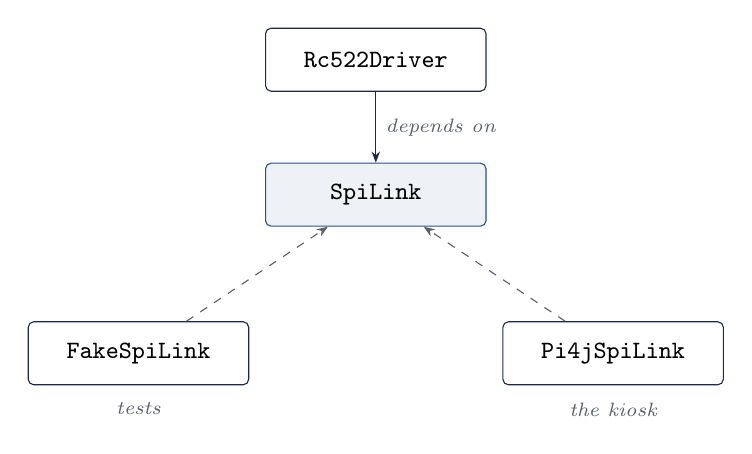
\begin{tikzpicture}[font=\footnotesize\sffamily,
   b/.style={draw=brewernavy, rounded corners=2pt, inner sep=5pt, minimum width=28mm, minimum height=8mm},
   i/.style={draw=brewerblue, fill=brewerblue!8, rounded corners=2pt, inner sep=5pt, minimum width=28mm, minimum height=8mm}]
  \node[b] (drv) {\code{Rc522Driver}};
  \node[i, below=9mm of drv] (if) {\code{SpiLink}};
  \node[b, below left=12mm and 2mm of if] (fake) {\code{FakeSpiLink}};
  \node[b, below right=12mm and 2mm of if] (real) {\code{Pi4jSpiLink}};
  \draw[-{Stealth[length=4pt]}, brewernavy] (drv) --
        node[right, font=\scriptsize\itshape, color=brewergrey] {depends on} (if);
  \draw[-{Stealth[length=4pt]}, dashed, brewergrey] (fake) -- (if);
  \draw[-{Stealth[length=4pt]}, dashed, brewergrey] (real) -- (if);
  \node[font=\scriptsize\itshape, color=brewergrey, below=1mm of fake] {tests};
  \node[font=\scriptsize\itshape, color=brewergrey, below=1mm of real] {the kiosk};
\end{tikzpicture}
\end{center}

In C you would get halfway there with a struct of function pointers, and the
idea is genuinely the same. Java's version is checked by the compiler: a class
that claims to satisfy the contract but forgets a method does not compile.

\section{Build it}

\subsection{\texttt{SpiException} --- the failure channel}

SPI can fail: the device file may not exist, a transfer can error. In C you
would return $-1$ and hope the caller checks.

\begin{jcode}
package com.midnightbrewer.hardware;

/**
 * Something went wrong talking to the SPI bus.
 *
 * Deliberately a CHECKED exception (extends Exception, not RuntimeException):
 * the compiler forces every caller to either handle it or declare that it
 * throws too. Hardware failure is not an edge case you get to forget about,
 * so we make the compiler nag.
 */
public class SpiException extends Exception {

    public SpiException(String message) {
        super(message);
    }

    public SpiException(String message, Throwable cause) {
        super(message, cause);   // keeps the original error's stack trace
    }
}
\end{jcode}

\begin{concept}{Checked exceptions are a design statement}
Java has two flavours of exception. \emph{Unchecked} ones
(\code{RuntimeException}) can be ignored silently. \emph{Checked} ones must be
acknowledged --- a caller either catches it or adds \code{throws SpiException} to
its own signature.

That distinction lets you encode a rule: \emph{the bus can fail, and you may not
forget that}. The cost is that \code{throws SpiException} propagates up your call
stack, which is a little noisy. But that noise is an accurate map of everything
in your program that can fail because hardware exists, and that map turns out to
be useful.
\end{concept}

The two-argument constructor matters more than it looks. \code{super(message,
cause)} preserves the underlying error, so when Pi4J throws some
\code{IOException} deep inside, you wrap it with your own context while keeping
the original stack trace. Debug output becomes ``my error, \emph{caused by}
their error'' rather than one or the other.

\subsection{\texttt{SpiLink} --- the contract}

\begin{jcode}
package com.midnightbrewer.hardware;

/**
 * The seam between this program and an SPI bus.
 *
 * An interface is a PROMISE, not code: any class that says "implements
 * SpiLink" must supply these methods, and the compiler enforces it.
 *
 * Everything above this line -- the driver, the reader, the whole card stack
 * -- depends only on this promise. Never on Pi4J, never on a device file.
 *
 * Extends AutoCloseable so callers can use try-with-resources and the RF
 * field is never left energised by a crash.
 */
public interface SpiLink extends AutoCloseable {

    /**
     * Full-duplex SPI transfer: shift out txBuffer, shift in rxBuffer.
     *
     * SPI is inherently full duplex -- every clock pulse sends a bit AND
     * receives a bit. So this is ONE method, not a send() and a receive().
     * The API mirrors the hardware rather than pretending it is a stream.
     */
    void transfer(byte[] txBuffer, byte[] rxBuffer, int length) throws SpiException;

    /** Release the bus. Overridden to narrow the exception type. */
    @Override
    void close() throws SpiException;
}
\end{jcode}

Notice there is \textbf{no code here at all} --- no fields, no bodies. An
interface is pure vocabulary, which is exactly why it makes a good seam: there
is nothing in it that could accidentally depend on a Pi.

\begin{deeper}{The signature is a design decision}
\code{transfer(tx, rx, length)} mirrors SPI's full-duplex reality: one call,
both directions. Had it been \code{send()} and \code{receive()}, every caller
would need to know that a ``read'' is really \emph{write the address, then clock
out a dummy byte to shift the answer in} --- a hardware detail leaking into every
call site.

Design the interface around what the hardware genuinely \emph{is}, and the code
above it stays honest. Design it around what feels convenient today, and you
spend next year translating.
\end{deeper}

\subsection{\texttt{FakeSpiLink} --- the test double}

This lives in \code{src/test/java/}, so it never ships.

\begin{jcode}
package com.midnightbrewer.hardware;

import java.util.ArrayList;
import java.util.HashMap;
import java.util.List;
import java.util.Map;

/**
 * A fake SPI bus: answers from a canned table, records what it was sent.
 *
 * This is the payoff of the interface. The driver cannot tell this from a real
 * Pi -- it only ever saw the SpiLink promise, and this keeps that promise.
 */
class FakeSpiLink implements SpiLink {

    /** Register address -> value the fake chip should report. */
    private final Map<Integer, Integer> registers = new HashMap<>();

    /** Every tx buffer we were handed, so a test can assert on it. */
    final List<byte[]> sent = new ArrayList<>();

    private boolean closed = false;

    void setRegister(int address, int value) { registers.put(address, value); }

    boolean isClosed() { return closed; }

    @Override
    public void transfer(byte[] txBuffer, byte[] rxBuffer, int length) {
        sent.add(txBuffer.clone());

        // TODO 1: decode the address byte the driver sent.
        //   A READ is encoded as ((addr << 1) & 0x7E) | 0x80, so:
        //     address = (txBuffer[0] & 0x7E) >> 1
        //     isRead  = (txBuffer[0] & 0x80) != 0

        // TODO 2: if it was a read, put the canned value in rxBuffer[1].
        //   The answer arrives on the SECOND byte: the first byte out is the
        //   address, and while that goes out the chip has nothing to say yet.
        //   Default to 0 for an address nobody configured.

        // TODO 3: if it was a write, there is nothing to answer.
    }

    @Override
    public void close() { closed = true; }
}
\end{jcode}

\begin{trap}{A fake that returns nothing}
If you leave \code{transfer()} empty, \code{rxBuffer} stays all zeros, your
driver dutifully returns \code{0}, and your test asserting \code{version() ==
0x92} fails --- so you go hunting for a bug in the driver that is not there.

Worse is the opposite: a test that \emph{passes} because both sides are
trivially empty.

\textbf{A fake must be a plausible liar, not a mute.} It has to behave enough
like the real thing that the code under test is genuinely exercised.
\end{trap}

\subsection{The test}

\begin{jcode}
package com.midnightbrewer.hardware;

import org.junit.jupiter.api.Test;
import static org.junit.jupiter.api.Assertions.assertEquals;
import static org.junit.jupiter.api.Assertions.assertTrue;

class FakeSpiLinkTest {

    @Test
    void readReturnsTheCannedValue() throws SpiException {
        FakeSpiLink link = new FakeSpiLink();
        link.setRegister(0x37, 0x92);          // VersionReg answers 0x92

        // Hand-encode a READ of register 0x37, exactly as the driver will.
        byte[] tx = { (byte) (((0x37 << 1) & 0x7E) | 0x80), 0x00 };
        byte[] rx = new byte[2];
        link.transfer(tx, rx, 2);

        assertEquals(0x92, rx[1] & 0xFF);      // & 0xFF -- the signed-byte thing
        assertEquals(1, link.sent.size());
    }

    @Test
    void closeIsRecorded() throws Exception {
        FakeSpiLink link = new FakeSpiLink();
        assertTrue(!link.isClosed());
        link.close();
        assertTrue(link.isClosed());
    }
}
\end{jcode}

\begin{verifybox}
\begin{shell}
mvn test -Dtest=FakeSpiLinkTest
\end{shell}
Green --- \emph{with the reader unplugged}. Pause on that: you have just tested
hardware-facing code with no hardware in the room.
\end{verifybox}

\subsection{\texttt{Pi4jSpiLink} --- the real one}

\begin{jcode}
package com.midnightbrewer.hardware;

import com.pi4j.Pi4J;
import com.pi4j.context.Context;
import com.pi4j.io.spi.Spi;
import com.pi4j.io.spi.SpiMode;

/**
 * The real SPI bus, via Pi4J and /dev/spidev0.0.
 *
 * The ONLY class in the project that knows Pi4J exists. Everything else sees
 * the SpiLink interface. Contain your dependencies in one place and swapping
 * them later is a one-file job.
 */
public class Pi4jSpiLink implements SpiLink {

    private static final int SPI_CHANNEL = 0;         // CE0
    private static final int SPI_BAUD    = 1_000_000; // 1 MHz

    private final Context pi4j;
    private final Spi spi;

    public Pi4jSpiLink() {
        this.pi4j = Pi4J.newAutoContext();
        this.spi = pi4j.create(Spi.newConfigBuilder(pi4j)
                .id("rc522")
                .address(SPI_CHANNEL)
                .baud(SPI_BAUD)
                .mode(SpiMode.MODE_0)   // RC522 is mode 0: CPOL=0, CPHA=0
                .build());
    }

    @Override
    public void transfer(byte[] txBuffer, byte[] rxBuffer, int length)
            throws SpiException {
        try {
            spi.transfer(txBuffer, 0, rxBuffer, 0, length);
        } catch (RuntimeException e) {
            throw new SpiException("SPI transfer failed", e);
        }
    }

    @Override
    public void close() throws SpiException {
        try {
            spi.close();
            pi4j.shutdown();
        } catch (RuntimeException e) {
            throw new SpiException("failed to close SPI", e);
        }
    }
}
\end{jcode}

\paragraph{Why 1\,MHz?} The MFRC522 handles 10\,MHz on a clean PCB. On loose
jumper wires it does not. 1\,MHz is fast enough that SPI is never your bottleneck
--- the card's RF timing dominates by orders of magnitude --- and slow enough to
tolerate imperfect wiring. Optimise the thing that is actually slow, not the
thing that is easy to measure.

\paragraph{Why mode 0?} CPOL${}=0$, CPHA${}=0$, from the datasheet: clock idles
low, data sampled on the rising edge. Get this wrong and you read
plausible-looking garbage, which is the worst kind of wrong.

\section{The concept, now that you have used it}
\index{dependency injection}

\textbf{Dependency injection} is the name for what you just did:
\code{Rc522Driver} will receive its \code{SpiLink} from outside, through its
constructor, rather than constructing one itself.

\begin{jcode}
// If the driver did this, it would be welded to the Pi forever:
class Rc522Driver {
    private final SpiLink link = new Pi4jSpiLink();   // untestable
}

// Handing it in from outside means the CALLER decides:
class Rc522Driver {
    private final SpiLink link;
    Rc522Driver(SpiLink link) { this.link = link; }   // testable
}
\end{jcode}

Same code, two power sources. The kettle does not own the power station.

\begin{concept}{A rule worth internalising}
\textbf{A class should not construct the things it depends on. It should be
handed them.}

``Who decides?'' moves up to whoever assembles the program, and testability,
flexibility and clear ownership all follow from that one move. When you meet a
class that is hard to test, look first for a \code{new} in its constructor.
\end{concept}

\section{Traps}

\begin{traptable}
\code{version()} returns $-110$ & Missing \code{\& 0xFF}. \hex{0x92} as a signed byte is $-110$. \\
Fake test passes, hardware returns 0 & The fake answers unconditionally; make it decode the address. \\
\code{NoClassDefFoundError: com/sun/jna/...} & JNA missing from the classpath. Run \code{mvn dependency:copy-dependencies}. \\
Works once, fails on the second run & You did not \code{close()}; the device file stays locked. Use try-with-resources. \\
\code{Permission denied} on \code{/dev/spidev0.0} & Not in the \code{spi} group. \code{sudo usermod -aG spi,gpio \$USER}. \\
\end{traptable}

\section{Commit}

\begin{shell}
git add -A
git commit -m "M1: SpiLink interface + fake and Pi4J implementations"
\end{shell}

\chapter{The RC522 driver}
\label{ch:driver}

\chapterbrief
  {Turn ``shift bytes over SPI'' into ``read and write named registers''.}
  {Encapsulation, and composition (HAS-A).}
  {A real chip reporting \code{version() == 0x92}.}

\section{The problem}

Reading one RC522 register over raw SPI looks like this:

\begin{jcode}
byte[] tx = { (byte) (((0x37 << 1) & 0x7E) | 0x80), 0x00 };
byte[] rx = new byte[2];
link.transfer(tx, rx, 2);
int version = rx[1] & 0xFF;
\end{jcode}

Five lines, three magic numbers, and a bit-twiddle you must get exactly right.
Now picture that at every one of the roughly forty register accesses in a card
transaction: two hundred lines of identical incantation, each an opportunity to
type \hex{0x7F} where you meant \hex{0x7E}.

\section{The idea: gather the mess in one place}
\index{encapsulation}

That is what a class is, at its most useful: \textbf{a place to put the mess so
the rest of the program does not have to know about it.} After this chapter the
rest of your program says

\begin{jcode}
int version = driver.version();
driver.antennaOn();
\end{jcode}

and the address encoding exists in exactly one place, written once, correct once.

\begin{analogy}{The steering wheel}
A car's steering wheel is an interface to a mess: a rack, a pinion, hydraulic
assist, tie rods, geometry that changes with speed. You turn a wheel.

You are not permitted to reach into the steering column mid-corner and adjust
the rack --- not because it is secret, but because the mechanism only works if it
is driven through the one sanctioned control.

\code{private} is that housing. It is not about hiding secrets; it is about
\textbf{guaranteeing that the only way to affect this thing is through the paths
you have thought about.}
\end{analogy}

\subsection{The address encoding}

From the MFRC522 datasheet, the first SPI byte is an address byte:

\begin{center}
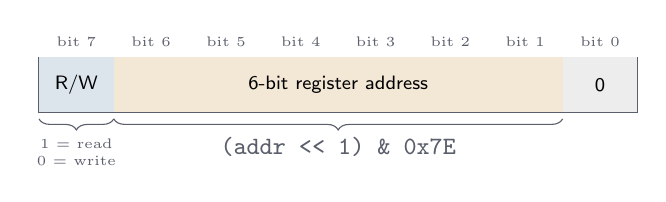
\begin{tikzpicture}[font=\scriptsize\sffamily, x=9.5mm, y=7mm]
  \foreach \i/\lbl in {0/7, 1/6, 2/5, 3/4, 4/3, 5/2, 6/1, 7/0}{
     \draw[draw=brewergrey] (\i,0) rectangle ++(1,1);
     \node[color=brewergrey, font=\tiny] at (\i+0.5, 1.28) {bit \lbl};
  }
  % RW bit
  \fill[brewerblue!16] (0,0) rectangle ++(1,1);
  \node at (0.5,0.5) {R/W};
  % address bits
  \fill[breweramber!16] (1,0) rectangle ++(6,1);
  \node at (4,0.5) {6-bit register address};
  % low bit
  \fill[black!7] (7,0) rectangle ++(1,1);
  \node at (7.5,0.5) {0};
  \draw[decorate, decoration={brace, amplitude=4pt, mirror}, brewergrey]
       (1,-0.12) -- (7,-0.12);
  \node[color=brewergrey, font=\tiny] at (4,-0.62) {\code{(addr << 1) \& 0x7E}};
  \draw[decorate, decoration={brace, amplitude=4pt, mirror}, brewergrey]
       (0,-0.12) -- (1,-0.12);
  \node[color=brewergrey, font=\tiny, align=center] at (0.5,-0.72) {1 = read\\0 = write};
\end{tikzpicture}
\end{center}

A register number must be shifted left one place to land in bits 6--1:

\begin{jcode}
((register << 1) & 0x7E) | 0x80    // read
 (register << 1) & 0x7E            // write
\end{jcode}

\code{\& 0x7E} is \code{0111 1110}: it masks off anything that overflowed past
bit 6 and forces bit 0 to zero. \code{| 0x80} sets the read flag. That is the
whole protocol, and after this chapter you never write it again.

\section{Build it}

\begin{jcode}
package com.midnightbrewer.hardware;

/**
 * The RC522 register-level driver.
 *
 * Encapsulation earns its keep here: the address encoding, the read/write bit
 * and the two-byte SPI dance all live IN HERE. The rest of the program calls
 * readRegister(0x37) and never writes ((reg << 1) & 0x7E) | 0x80 again.
 */
public class Rc522Driver {

    // ---- register addresses (MFRC522 datasheet, section 9) ----
    private static final int COMMAND_REG    = 0x01;  // CommandReg
    private static final int TX_CONTROL_REG = 0x14;  // TxControlReg (antenna)
    private static final int VERSION_REG    = 0x37;  // VersionReg (0x91 / 0x92)

    private static final int PCD_SOFT_RESET = 0x0F;  // the SoftReset command

    // ---- composition: the driver HAS-A SpiLink ----
    //
    // 'private' = nobody outside can reach past the driver and touch the bus.
    // 'final'   = once set in the constructor, this never points elsewhere.
    // The type is the INTERFACE, so the driver cannot tell real from fake.
    private final SpiLink link;

    // Dependency injection: the bus is handed in, not constructed here.
    public Rc522Driver(SpiLink link) {
        this.link = link;
    }

    // =================================================================
    // readRegister
    //
    //   C:  uchar Read_MFRC522(uchar addr) {
    //           SPI_Transfer( ((addr<<1)&0x7E) | 0x80 );  // address, read bit
    //           val = SPI_Transfer(0x00);                 // 2nd byte = answer
    //           return val;
    //       }
    //
    //   In Java ONE transfer() moves both bytes: build a 2-byte tx (encoded
    //   address, then 0x00), a 2-byte rx, call link.transfer, answer in rx[1].
    //   Return it masked with & 0xFF so 0x92 comes back as 146, not -110.
    // =================================================================
    public int readRegister(int register) throws SpiException {
        // TODO
        return 0;
    }

    // =================================================================
    // writeRegister
    //
    //   Same shape, two differences: the address byte does NOT set 0x80
    //   (that is what makes it a write), and the second byte is the value
    //   instead of 0x00. Nothing to read back.
    // =================================================================
    public void writeRegister(int register, int value) throws SpiException {
        // TODO
    }

    // =================================================================
    // setBitMask -- turn bits ON without disturbing the others.
    //
    //   C:  tmp = Read(reg);  Write(reg, tmp | mask);
    //
    //   "Read-modify-write". Build it from the two methods you just wrote,
    //   NOT from link.transfer. Each layer uses only the layer below it.
    // =================================================================
    public void setBitMask(int register, int mask) throws SpiException {
        // TODO
    }

    /** Turn bits OFF: same shape, but AND with ~mask. */
    public void clearBitMask(int register, int mask) throws SpiException {
        // TODO
    }

    /** Write the SoftReset command to CommandReg. One line. */
    public void softReset() throws SpiException {
        // TODO
    }

    // =================================================================
    // antennaOn -- power up the RF field.
    //
    //   C:  Read_MFRC522(TxControlReg);      // the C reads and ignores it
    //       SetBitMask(TxControlReg, 0x03);  // Tx1RFEn | Tx2RFEn
    //
    //   The two low bits of TxControlReg are the antenna drivers. Watch the
    //   register go 0x80 -> 0x83; that is read-modify-write doing its job.
    // =================================================================
    public void antennaOn() throws SpiException {
        // TODO
    }

    /** The chip's version byte: 0x91 (v1.0) or 0x92 (v2.0). */
    public int version() throws SpiException {
        // TODO
        return 0;
    }
}
\end{jcode}

\begin{concept}{Each layer uses only the layer beneath it}
\code{setBitMask} could call \code{link.transfer} directly and it would work.
Do not.

If you shortcut a layer you have created a second path to the same hardware ---
and the day you need to add logging, retries, or a mutex to register access, one
path gets it and the other silently does not. That is not a hypothetical; it is
precisely how ``I fixed the bug but it still happens sometimes'' bugs are born.
\end{concept}

\section{Verify --- with no hardware}

\begin{jcode}
package com.midnightbrewer.hardware;

import org.junit.jupiter.api.Test;
import static org.junit.jupiter.api.Assertions.assertEquals;

class Rc522DriverTest {

    @Test
    void readsTheVersionRegister() throws SpiException {
        FakeSpiLink link = new FakeSpiLink();
        link.setRegister(0x37, 0x92);

        Rc522Driver driver = new Rc522Driver(link);

        assertEquals(0x92, driver.version());
    }

    @Test
    void writeEncodesTheAddressWithoutTheReadBit() throws SpiException {
        FakeSpiLink link = new FakeSpiLink();
        Rc522Driver driver = new Rc522Driver(link);

        driver.writeRegister(0x14, 0x03);

        byte[] tx = link.sent.get(0);
        assertEquals((0x14 << 1) & 0x7E, tx[0] & 0xFF);   // read bit CLEAR
        assertEquals(0x03, tx[1] & 0xFF);
    }
}
\end{jcode}

The second test is the interesting one: it asserts on \textbf{what went out on
the wire}, which is the only way to catch an encoding bug. A test that checked
only return values would happily pass with the read bit set on a write.

\begin{verifybox}
\begin{shell}
mvn test -Dtest=Rc522DriverTest
\end{shell}
\end{verifybox}

\section{Now the real chip}

\begin{jcode}
package com.midnightbrewer.hardware;

public final class HardwareCheck {

    private HardwareCheck() { }

    public static void main(String[] args) throws Exception {
        System.out.println("Opening the reader...");

        try (Pi4jSpiLink link = new Pi4jSpiLink()) {
            Rc522Driver driver = new Rc522Driver(link);

            driver.softReset();
            Thread.sleep(50);              // the chip needs a moment after reset
            driver.antennaOn();

            int version = driver.version();
            System.out.printf("version() = 0x%02X%n", version);
            if (version == 0x91 || version == 0x92) {
                System.out.println("  -> the driver works on silicon.");
            } else {
                System.out.println("  -> chip not answering. Check wiring/power.");
            }
        }
    }
}
\end{jcode}

\begin{shell}
# on your laptop
rsync -av --exclude target/ ./ martin@raspberrypi.local:~/midnight-brewer/

# on the Pi
cd ~/midnight-brewer
mvn -q -DskipTests compile dependency:copy-dependencies -DincludeScope=runtime
java -cp "target/classes:target/dependency/*" \
     com.midnightbrewer.hardware.HardwareCheck
\end{shell}

\begin{verifybox}
\begin{trace}
version() = 0x92
  -> the driver works on silicon.
\end{trace}
\end{verifybox}

\subsection{If you get \texttt{0x00} or \texttt{0xFF}}

Those are the two ``nobody home'' values, and they are diagnostic:

\begin{itemize}
  \item \hex{0x00} --- MISO stuck low. Usually MISO not connected, chip
        unpowered, or CS on the wrong pin.
  \item \hex{0xFF} --- MISO stuck high, i.e.\ floating. Usually MISO connected
        to nothing, or a dead chip.
\end{itemize}

Check power first (3.3\,V, \emph{not} 5\,V), then wiring, then shorten your
wires. Do not debug the code: it is ten lines and your test already proved it.

\begin{deeper}{try-with-resources, and why \texttt{AutoCloseable} mattered}
\code{try (Pi4jSpiLink link = ...)} calls \code{close()} when the block exits ---
normally, by exception, or by early return. That is why \code{SpiLink extends
AutoCloseable} back in Chapter~\ref{ch:spi}.

On a kiosk it means a crash can never leave the RF field energised, which is
the sort of thing that quietly cooks a reader module overnight. Resource cleanup
that depends on remembering to write it is resource cleanup that eventually does
not happen.
\end{deeper}

\section{Traps}

\begin{traptable}
\code{version()} $= -110$ & Missing \code{\& 0xFF}. \\
\code{version()} $=$ \hex{0x00} & MISO low: power, wiring, or wrong CS pin. \\
\code{version()} $=$ \hex{0xFF} & MISO floating: not connected. \\
Reads work, writes do not & Read bit \hex{0x80} accidentally set on writes. \\
Fine on the bench, flaky when mounted & Wire length. Shorten them. \\
\hex{0x92} in the test, \hex{0x00} on the Pi & Stale \code{target/}. Run \code{mvn clean compile}. \\
\end{traptable}

\section{Commit}

\begin{shell}
git add -A
git commit -m "M2: Rc522Driver -- register read/write, bitmasks, reset, antenna"
\end{shell}


\part{Talking to the Card}
\chapter{The reader base class}
\label{ch:reader}

\chapterbrief
  {Send a frame to a card and get its answer back.}
  {Abstract classes, and the Template Method pattern.}
  {\code{isCardPresent()} detecting a real DESFire.}

\section{The problem}

You can read registers. Now you need to \emph{talk to a card}, which means a
fixed sequence: tell the chip how many bits are in the last byte, flush the
FIFO, clear old interrupt flags, load the outgoing bytes, start the transceive
command, wait for a reply or a timeout, check the error register, and read the
reply out.

Here is the thing: \textbf{those steps are RC522-specific, but the protocol
above them is not.} ``Send REQA, expect a two-byte ATQA'' is ISO-14443 ---
identical on a PN532, a PN5180, or an ACR122. Write the protocol logic
\emph{inside} an RC522 class and you must rewrite all of it to support a second
chip.

\section{The idea: leave a hole in the middle of the algorithm}
\index{Template Method}

Write the protocol once, in a base class, and leave the chip-specific step
\textbf{blank} --- a method with a name and a signature but no body. Subclasses
fill the blank. The base class calls the blank as if it were already written.

That is the \textbf{Template Method} pattern: the parent owns the \emph{shape}
of the algorithm, the children supply the \emph{steps}.

\begin{analogy}{The recipe with one variable step}
A stir-fry recipe: heat the oil, \textbf{cook the protein}, add vegetables, add
sauce, serve. The sequence is fixed --- you never add sauce before the oil is hot.

But ``cook the protein'' is a hole. Chicken takes six minutes, prawns two, tofu
wants pressing first. The cookbook writes the sequence; the specific dish fills
the hole.

Critically, the recipe \emph{calls} the hole without knowing what goes in it.
\code{isCardPresent()} calls \code{transceive()}, and at runtime that call lands
in \code{Rc522Reader}, or \code{Pn532Reader}, or a fake. The base class never
learns which.
\end{analogy}

\begin{center}
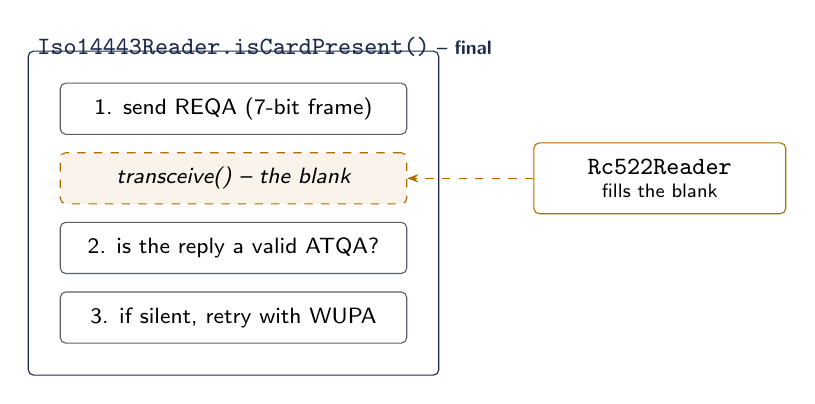
\begin{tikzpicture}[font=\footnotesize\sffamily,
  tstep/.style={draw=brewergrey, rounded corners=2pt, minimum width=44mm,
               minimum height=6.5mm, inner sep=3pt},
  hole/.style={draw=breweramber, dashed, fill=breweramber!8, rounded corners=2pt,
               minimum width=44mm, minimum height=6.5mm, inner sep=3pt}]
  \node[tstep] (s1) {1. send REQA (7-bit frame)};
  \node[hole, below=2.2mm of s1] (h1) {\itshape transceive() -- the blank};
  \node[tstep, below=2.2mm of h1] (s2) {2. is the reply a valid ATQA?};
  \node[tstep, below=2.2mm of s2] (s3) {3. if silent, retry with WUPA};
  \node[draw=brewernavy, rounded corners=2pt, fit=(s1)(s3), inner sep=4mm] (box) {};
  \node[font=\scriptsize\sffamily\bfseries, color=brewernavy, above=0.5mm of box.north west,
        anchor=west] {\code{Iso14443Reader.isCardPresent()} -- final};
  \node[draw=breweramber, rounded corners=2pt, right=16mm of h1,
        minimum width=32mm, minimum height=9mm, inner sep=3pt,
        align=center, font=\scriptsize\sffamily] (impl)
        {\code{Rc522Reader}\\ fills the blank};
  \draw[-{Stealth[length=4pt]}, breweramber, dashed] (impl) -- (h1);
\end{tikzpicture}
\end{center}

\subsection{Why an abstract class and not an interface}
\index{abstract class}

An interface holds method signatures but no state. Here you need \emph{both}:
real shared code (the protocol) \emph{and} a blank (the chip step). That mix is
exactly what an abstract class is for.

\begin{center}\small
\begin{tabular}{@{}lcc@{}}
\toprule
 & \thead{interface} & \thead{abstract class} \\
\midrule
Method signatures    & yes & yes \\
Real method bodies   & mostly no & yes \\
Fields / state       & no  & yes \\
Can be instantiated  & no  & no  \\
A class can have many & yes & no (one parent) \\
\bottomrule
\end{tabular}
\end{center}

\begin{concept}{Which one to reach for}
\textbf{Interface} = ``can do this'' --- a capability, like \code{SpiLink}.

\textbf{Abstract class} = ``is a kind of this'' --- a family sharing machinery,
like \code{Iso14443Reader}.
\end{concept}

\section{Build it}

\subsection{The base}

\begin{jcode}
package com.midnightbrewer.hardware;

/**
 * An abstract base for any ISO-14443 reader.
 *
 * The protocol logic is a standard: identical for an RC522, a PN532, anything.
 * That logic lives HERE, written once. What differs per chip is only how you
 * physically push a frame out and read the reply -- left BLANK for each chip's
 * subclass to fill.
 */
public abstract class Iso14443Reader {

    // ---- ISO 14443-3 constants (chip-independent) ----
    private static final byte REQA = 0x26; // "any IDLE card, announce yourself"
    private static final byte WUPA = 0x52; // "any IDLE *or* HALTed card, wake up"

    /** A valid ATQA answer is exactly two bytes. */
    private static final int ATQA_LENGTH = 2;

    /** REQA/WUPA are 7-bit short frames, not whole bytes. */
    private static final int REQA_BITS = 7;

    // =================================================================
    // THE BLANK. 'abstract' = declared, no body. A subclass MUST supply
    // one or it will not compile.
    //
    //   sendData       : bytes to transmit
    //   bitsInLastByte : valid bits in the final byte (7 for REQA, 0 = all 8)
    //   returns        : bytes received, or an EMPTY array if nothing answered.
    //
    // Note "empty array" rather than an exception: a timeout is NORMAL when no
    // card is on the antenna. Exceptions are for the exceptional.
    // =================================================================
    protected abstract byte[] transceive(byte[] sendData, int bitsInLastByte)
            throws SpiException;

    /**
     * The second blank: compute the 2-byte CRC_A over data.
     *
     * SELECT and RATS need a CRC appended; anticollision does not. The RC522
     * has a hardware CRC unit, another chip might not -- so, like transceive,
     * it is left for the subclass. An abstract class may carry as many blanks
     * as the design needs.
     *
     * @return two CRC bytes, low first, ready to append.
     */
    protected abstract byte[] calculateCrc(byte[] data) throws SpiException;

    // =================================================================
    // THE TEMPLATE METHOD -- the fixed algorithm, shared by all chips.
    //
    // 'final' on purpose: a subclass may fill the blanks, but may NOT rewrite
    // the sequence. The protocol is the protocol.
    // =================================================================
    public final boolean isCardPresent() throws SpiException {
        // TODO 1: try REQA; if that finds a card, return true.
        // TODO 2: otherwise try WUPA and return that result.
        //
        //   Why both? REQA only wakes cards in IDLE. A card you already talked
        //   to sits in HALT and ignores REQA forever -- WUPA wakes those too.
        //   Without this, the reader works ONCE and then goes blind until the
        //   card is physically removed and replaced.
        return false;
    }

    /** Sends one REQA/WUPA and reports whether a well-formed ATQA came back. */
    private boolean request(byte mode) throws SpiException {
        // TODO: transceive a single-byte frame { mode } with REQA_BITS bits,
        //       and return whether the reply length == ATQA_LENGTH.
        return false;
    }
}
\end{jcode}

\begin{concept}{\texttt{public}, \texttt{protected}, \texttt{private}}
\code{protected} means ``visible to this class and its subclasses, but not the
outside world''. \code{transceive} is an implementation detail of the reader
family --- the kiosk should never call it.

\textbf{\code{public} for the vocabulary, \code{protected} for the family,
\code{private} for the class alone.} Choosing these deliberately is most of what
designing a class \emph{is}.

And \code{final} on \code{isCardPresent()} encodes a design decision in the type
system: \emph{chips vary, the standard does not.} Deciding what subclasses may
and may not change is the real work of writing a base class.
\end{concept}

\subsection{The RC522 subclass}

\begin{jcode}
package com.midnightbrewer.hardware;

/**
 * The RC522's answer to the two blanks in Iso14443Reader.
 *
 * 'extends' = inheritance: this IS-A Iso14443Reader and gets all its protocol
 * code for free. It supplies only the two chip-specific steps.
 */
public class Rc522Reader extends Iso14443Reader {

    // ---- registers this needs ----
    private static final int COMMAND_REG     = 0x01;
    private static final int COMM_IEN_REG    = 0x02; // which IRQs are enabled
    private static final int COMM_IRQ_REG    = 0x04; // which IRQs have fired
    private static final int ERROR_REG       = 0x06;
    private static final int FIFO_DATA_REG   = 0x09; // the FIFO, in and out
    private static final int FIFO_LEVEL_REG  = 0x0A; // bytes currently in it
    private static final int BIT_FRAMING_REG = 0x0D; // TxLastBits + StartSend

    private static final int PCD_IDLE       = 0x00; // "cancel / do nothing"
    private static final int PCD_TRANSCEIVE = 0x0C; // "send the FIFO, receive"

    // ---- CRC coprocessor ----
    private static final int DIV_IRQ_REG      = 0x05; // CRCIrq is bit 2
    private static final int CRC_RESULT_REG_L = 0x22;
    private static final int CRC_RESULT_REG_H = 0x21;
    private static final int PCD_CALCCRC      = 0x03;

    // COMPOSITION again: the reader HAS-A driver. Note it does NOT extend
    // Rc522Driver -- a reader is not a kind of driver, it USES one.
    private final Rc522Driver driver;

    public Rc522Reader(Rc522Driver driver) {
        this.driver = driver;
    }

    @Override
    protected byte[] transceive(byte[] sendData, int bitsInLastByte)
            throws SpiException {

        // ---- 1. how many bits are valid in the last byte ----
        //   C: Write(BitFramingReg, 0x07);   // 7 for REQA
        // TODO: writeRegister(BIT_FRAMING_REG, bitsInLastByte & 0x07);

        // ---- 2. arm the chip and empty the FIFO ----
        //   C: Write(CommIEnReg, 0x77|0x80);   // enable IRQs
        //      ClearBitMask(CommIrqReg, 0x80); // clear old flags
        //      SetBitMask(FIFOLevelReg, 0x80); // flush FIFO
        //      Write(CommandReg, PCD_IDLE);    // cancel running command
        // TODO: those four calls.

        // ---- 3. load the outgoing bytes into the FIFO ----
        // TODO: a loop writing each byte of sendData to FIFO_DATA_REG
        //       (as an int: sendData[i] & 0xFF).

        // ---- 4. run it, and press "start sending" ----
        //   C: Write(CommandReg, PCD_TRANSCEIVE);
        //      SetBitMask(BitFramingReg, 0x80);   // StartSend = bit 7
        // TODO: those two.

        // ---- 5. wait for the answer, or a timeout ----
        //   The C spins a large counter. That does NOT port -- see the note
        //   below. Use a WALL-CLOCK deadline:
        //
        //   long deadline = System.nanoTime() + 50_000_000L;   // ~50 ms
        //   int irq;
        //   do {
        //       irq = driver.readRegister(COMM_IRQ_REG);
        //   } while (System.nanoTime() < deadline
        //            && (irq & 0x01) == 0      // TimerIRq -> nobody answered
        //            && (irq & 0x30) == 0);    // RxIRq|IdleIRq -> done
        // TODO: the loop. Keep 'irq' -- step 6 needs it.

        // ---- 6. stop sending, then check for trouble ----
        //   C: ClearBitMask(BitFramingReg, 0x80);
        //      if (Read(ErrorReg) & 0x1B) ...   // overflow, parity, CRC, protocol
        //   Also: if TimerIRq fired, nobody answered.
        //   Either way return an EMPTY array -- "no card" is not an error.
        // TODO.

        // ---- 7. read the reply out of the FIFO ----
        //   C: n = Read(FIFOLevelReg);
        //      for (i=0;i<n;i++) backData[i] = Read(FIFODataReg);
        // TODO: read the level into n, allocate byte[n], loop reading
        //       FIFO_DATA_REG into each slot, return it.
        //
        //   Note: you read the SAME register n times. It is a FIFO -- each
        //   read pops the next byte. This looks wrong and is right.
        return new byte[0];
    }

    @Override
    protected byte[] calculateCrc(byte[] data) throws SpiException {
        //   C: Write(CommandReg, PCD_IDLE);
        //      ClearBitMask(DivIrqReg, 0x04);   // clear CRCIrq
        //      SetBitMask(FIFOLevelReg, 0x80);  // flush FIFO
        //      for (i..) Write(FIFODataReg, data[i]);
        //      Write(CommandReg, PCD_CALCCRC);
        //      wait for DivIrqReg bit 2
        //      out[0] = Read(CRCResultRegL);  out[1] = Read(CRCResultRegH);
        //
        // TODO all of it. Same wall-clock trick (~20 ms is plenty).
        // Return { low, high }: ISO-14443 puts the CRC on the wire low byte
        // first, and returning it wire-ready means callers just append it.
        return new byte[2];
    }
}
\end{jcode}

\section{The two ports that do not survive translation}

\begin{trap}{Iteration counts become deadlines}
The single most important lesson in porting embedded C to Linux.

\code{for (i = 0; i < 2000; i++)} on bare metal is microseconds. Here, each
iteration is a \code{readRegister}, which is a syscall through the kernel --- on
the order of 50\,\textmu s. The same loop count runs for \emph{minutes}.

Always time out on \code{System.nanoTime()}, never on a loop counter. If your
program appears to hang, this is the first thing to check.
\end{trap}

Second: \textbf{chip-select is no longer yours}. The C toggles CS around each
byte. Your \code{SpiLink.transfer()} already performs one complete, atomic
transaction. Try to manage CS yourself and you will fight the kernel driver and
lose.

\section{Verify on hardware}

Before polling, the chip needs a full init sequence --- the datasheet defaults
are not usable:

\begin{jcode}
private static void initChip(Rc522Driver driver) throws SpiException {
    driver.writeRegister(0x2A, 0x8D); // TModeReg     } response timer,
    driver.writeRegister(0x2B, 0x3E); // TPrescalerReg} ~300 ms at 6.78 MHz
    driver.writeRegister(0x2C, 0x02); // TReloadRegH  } (0x0258 = 600 ticks)
    driver.writeRegister(0x2D, 0x58); // TReloadRegL  }
    driver.writeRegister(0x15, 0x40); // TxASKReg  -> force 100% ASK modulation
    driver.writeRegister(0x11, 0x3D); // ModeReg   -> CRC preset 0x6363
    driver.writeRegister(0x26, 0x08); // RFCfgReg  -> receiver gain
    driver.antennaOn();
}
\end{jcode}

Two of those matter enormously:

\begin{itemize}
  \item \reg{TxASKReg} $=$ \hex{0x40} forces 100\,\% ASK modulation, which
        Type~A cards require. Without it the card never sees a valid signal, and
        you get a silence that looks exactly like a wiring fault.
  \item \reg{ModeReg} $=$ \hex{0x3D} sets the CRC preset to \hex{0x6363}, the
        ISO-14443-A value. Wrong preset means every CRC you compute is wrong,
        so every SELECT is rejected --- in Chapter~\ref{ch:activation}, not here,
        which makes it maddening to trace.
\end{itemize}

\begin{jcode}
Rc522Reader reader = new Rc522Reader(driver);
System.out.println("Polling 15x (put a card on the antenna)...");
int hits = 0;
for (int i = 0; i < 15; i++) {
    if (reader.isCardPresent()) hits++;
    Thread.sleep(40);
}
System.out.printf("card detected in %d / 15 polls%n", hits);
\end{jcode}

\begin{verifybox}
\begin{trace}
card detected in 15 / 15 polls
\end{trace}
If you get \code{0/15} with a card sitting on the antenna, check the init
sequence first --- especially those two registers --- then confirm the card is
actually 13.56\,MHz.
\end{verifybox}

\section{Traps}

\begin{traptable}
Runs for minutes, no output & Ported the C's iteration counter. Use a \code{nanoTime} deadline. \\
\code{0/15} polls, chip version fine & Missing \reg{TxASKReg}$=$\hex{0x40} or \reg{ModeReg}$=$\hex{0x3D}. \\
Detects once, then never again & Only sending REQA. Halted cards need WUPA. \\
Detection works about half the time & Wire length, or card not flat on the antenna. \\
\code{NegativeArraySizeException} & FIFO level read before the reply arrived --- check the wait loop. \\
\end{traptable}

\section{Commit}

\begin{shell}
git add -A
git commit -m "M3: Iso14443Reader template method + Rc522Reader transceive/CRC"
\end{shell}

\chapter{Protocol blocks}
\label{ch:blocks}

\chapterbrief
  {Model the three ISO-14443-4 frame types as a small class hierarchy.}
  {Inheritance, polymorphism, and the factory method.}
  {A three-class hierarchy with tests, and one place where type is decided.}

\section{The problem}

Once a card is activated you exchange \textbf{T=CL blocks}. Every frame starts
with a PCB (Protocol Control Byte) whose top bits say which of three kinds it is:

\begin{center}\small
\begin{tabular}{@{}llll@{}}
\toprule
\thead{PCB bits} & \thead{Type} & \thead{Carries} & \thead{Purpose} \\
\midrule
\code{0xxxxxxx}  & \textbf{I-block} (Information) & your APDU & the actual data \\
\code{10xxxxxx}  & \textbf{R-block} (Receive ready) & nothing & acknowledgement \\
\code{11xxxxxx}  & \textbf{S-block} (Supervisory) & control info & ``wait'', ``deselect'' \\
\bottomrule
\end{tabular}
\end{center}

The C approach is a switch statement, and it works fine --- \emph{once}. The
problem is what happens over time. You need \code{describe()} for logging: one
switch. Then \code{expectsResponse()}: a second. Then \code{encode()}: a third.
Now three switches must be kept in agreement, and when a fourth block type
appears you must find all of them.

That is the smell: \textbf{the type of a thing is being re-decided at every place
you use it.}

\section{The idea: decide once, then let the object know what it is}

Make each block type a class. Decide which one you are holding \emph{exactly
once}, at the moment the byte arrives. Afterwards you hold an object that already
knows what it is, and you just call methods on it.

\begin{analogy}{The parcel depot}
A parcel arrives. You could sort it at every stage --- check ``is this fragile?''
at the truck, again at the belt, again at the van. Or you sort \emph{once} at
intake, put it in the right bin, and afterwards every stage handles ``whatever is
in this bin'' by that bin's rules.

One decision point, made once, near the door. The factory method is the intake
desk; polymorphism is the bin's rules applying automatically.
\end{analogy}

\begin{center}
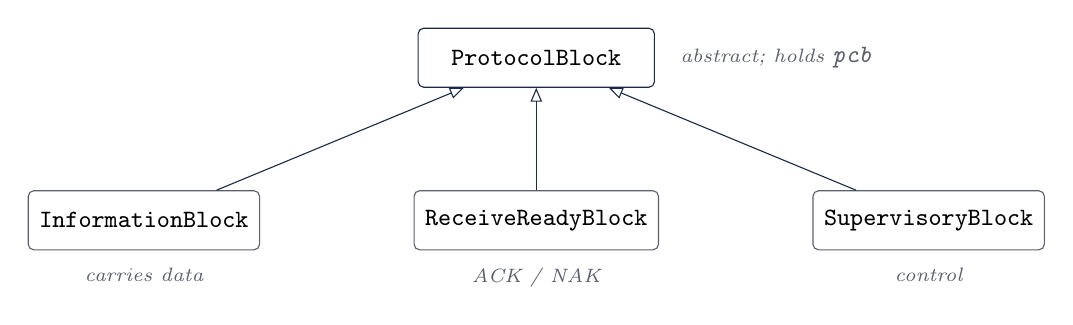
\begin{tikzpicture}[font=\footnotesize\sffamily,
  b/.style={draw=brewernavy, rounded corners=2pt, inner sep=4pt,
            minimum width=30mm, minimum height=7.5mm},
  sub/.style={draw=brewergrey, rounded corners=2pt, inner sep=4pt,
            minimum width=27mm, minimum height=7.5mm}]
  \node[b] (base) {\code{ProtocolBlock}};
  \node[font=\scriptsize\itshape, color=brewergrey, right=2mm of base]
       {abstract; holds \code{pcb}};
  \node[sub, below left=13mm and 20mm of base] (i) {\code{InformationBlock}};
  \node[sub, below=13mm of base] (r) {\code{ReceiveReadyBlock}};
  \node[sub, below right=13mm and 20mm of base] (sb) {\code{SupervisoryBlock}};
  \foreach \n in {i, r, sb}{
    \draw[-{Triangle[open, length=5pt]}, brewernavy] (\n) -- (base);}
  \node[font=\scriptsize\itshape, color=brewergrey, below=1mm of i] {carries data};
  \node[font=\scriptsize\itshape, color=brewergrey, below=1mm of r] {ACK / NAK};
  \node[font=\scriptsize\itshape, color=brewergrey, below=1mm of sb] {control};
\end{tikzpicture}
\end{center}

\begin{concept}{Polymorphism}
\index{polymorphism}
Literally ``many shapes''. You call \code{block.describe()}. Java looks at what
the object \emph{actually is} at runtime --- I, R or S --- and runs that class's
version.

One call site, three behaviours, and no \code{if} anywhere.
\end{concept}

\section{Build it}

\subsection{The base}

\begin{jcode}
package com.midnightbrewer.hardware;

/**
 * One ISO-14443-4 (T=CL) block.
 *
 * All three types share the PCB, so that state lives here in the base -- which
 * is exactly why this is an abstract CLASS and not an interface (an interface
 * cannot hold the field).
 *
 * What DIFFERS is behaviour, so describe() is abstract: each subclass answers
 * it its own way.
 */
public abstract class ProtocolBlock {

    private final int pcb;

    // 'protected' -- only subclasses construct blocks, via the factory below.
    protected ProtocolBlock(int pcb) {
        this.pcb = pcb & 0xFF;
    }

    /** The raw PCB byte (0..255). */
    public int pcb() {
        return pcb;
    }

    /** Declared here, no body -- every subclass MUST answer. */
    public abstract String describe();

    // =================================================================
    // THE FACTORY -- the ONE place the type is decided.
    //
    // This switch exists once, here. Everywhere else you hold a
    // ProtocolBlock and call methods on it. No type checks, no instanceof.
    //
    //   b8 = 0         -> I-block
    //   b8 = 1, b7 = 0 -> R-block
    //   b8 = 1, b7 = 1 -> S-block
    // =================================================================
    public static ProtocolBlock from(int pcb) {
        // TODO 1: if bit 7 (0x80) is clear      -> new InformationBlock(pcb)
        // TODO 2: else if bit 6 (0x40) is clear -> new ReceiveReadyBlock(pcb)
        // TODO 3: else                          -> new SupervisoryBlock(pcb)
        return null;
    }
}
\end{jcode}

\begin{concept}{Why a static factory instead of \texttt{new}}
Because the caller does not know which class it wants --- that is precisely what
it is asking. \code{ProtocolBlock.from(0x02)} says ``give me whatever block this
byte represents''. The caller states intent; the factory decides the type.

This is the \textbf{Open/Closed Principle} in miniature: to add a block type you
add a class and one line in the factory. Every existing call site keeps working,
untouched. Compare the switch-everywhere version, where you must hunt through the
codebase and hope you found them all.
\end{concept}

\subsection{The three subclasses}

\begin{jcode}
package com.midnightbrewer.hardware;

public class InformationBlock extends ProtocolBlock {

    public InformationBlock(int pcb) {
        super(pcb);          // hand the PCB up to the base to store
    }

    @Override
    public String describe() {
        // TODO: "I-block (data), block number N"
        //       The block number is the low bit: pcb() & 0x01
        return null;
    }
}
\end{jcode}

\begin{jcode}
public class ReceiveReadyBlock extends ProtocolBlock {

    public ReceiveReadyBlock(int pcb) { super(pcb); }

    @Override
    public String describe() {
        // TODO: "R-block (ACK)" or "R-block (NAK)" -- bit 4 (0x10) set = NAK.
        return null;
    }
}
\end{jcode}

\begin{jcode}
public class SupervisoryBlock extends ProtocolBlock {

    public SupervisoryBlock(int pcb) { super(pcb); }

    @Override
    public String describe() {
        // TODO: bits 5..4 (mask 0x30) say which:
        //         0x00 -> "S-block (DESELECT)"
        //         0x30 -> "S-block (WTX -- card asking for more time)"
        //         else -> "S-block (unknown)"
        return null;
    }
}
\end{jcode}

\code{super(pcb)} calls the parent's constructor, and it must be the first
statement: the base must be fully built before the subclass adds to it.
Foundations before walls.

\begin{concept}{Always write \texttt{@Override}}
It is optional, and you should write it anyway. It tells the compiler ``I mean
to be replacing a parent method''. If you typo \code{describ()}, you get a
compile error instead of a method that silently never gets called. Free
insurance against a genuinely baffling class of bug.
\end{concept}

\section{Verify}

\begin{jcode}
package com.midnightbrewer.hardware;

import org.junit.jupiter.api.Test;
import static org.junit.jupiter.api.Assertions.assertEquals;
import static org.junit.jupiter.api.Assertions.assertTrue;

class ProtocolBlockTest {

    @Test
    void factoryPicksTheRightType() {
        assertTrue(ProtocolBlock.from(0x02) instanceof InformationBlock);
        assertTrue(ProtocolBlock.from(0x03) instanceof InformationBlock);
        assertTrue(ProtocolBlock.from(0xA2) instanceof ReceiveReadyBlock);
        assertTrue(ProtocolBlock.from(0xF2) instanceof SupervisoryBlock);
    }

    @Test
    void polymorphicDescribe() {
        // Same variable type, same method call, three different answers.
        ProtocolBlock[] blocks = {
            ProtocolBlock.from(0x02),
            ProtocolBlock.from(0xA2),
            ProtocolBlock.from(0xF2),
        };
        assertTrue(blocks[0].describe().startsWith("I-block"));
        assertTrue(blocks[1].describe().startsWith("R-block"));
        assertTrue(blocks[2].describe().startsWith("S-block"));

        assertEquals(0, ProtocolBlock.from(0x02).pcb() & 0x01);
        assertEquals(1, ProtocolBlock.from(0x03).pcb() & 0x01);
    }
}
\end{jcode}

Look closely at \code{polymorphicDescribe}: the array's type is
\code{ProtocolBlock[]}. The code calling \code{describe()} has \textbf{no idea}
which subclass each element is, and does not need to. That is the entire point.

\begin{deeper}{\texttt{instanceof} in tests versus in production}
Using \code{instanceof} in the first test is fine --- a test's job is to verify
the factory picks correctly.

\code{instanceof} in \emph{production} code is usually a signal that you should
have added a method to the base instead. If you find yourself writing
\code{if (b instanceof InformationBlock) \{ ... \}}, ask what question you are
really asking, and give the base class a method that answers it.
\end{deeper}

\begin{verifybox}
\begin{shell}
mvn test -Dtest=ProtocolBlockTest
\end{shell}
\end{verifybox}

\section{Inheritance versus composition}
\index{composition}\index{inheritance}

You have now used both ways one class can relate to another:

\begin{itemize}
  \item \textbf{Composition (HAS-A)} --- \code{Rc522Reader} \emph{has a}
        \code{Rc522Driver}; \code{Rc522Driver} \emph{has a} \code{SpiLink}.
  \item \textbf{Inheritance (IS-A)} --- \code{Rc522Reader} \emph{is a}
        \code{Iso14443Reader}; \code{InformationBlock} \emph{is a}
        \code{ProtocolBlock}.
\end{itemize}

The test is whether ``IS-A'' is literally true. An I-block \emph{is a} protocol
block --- yes. Is a reader \emph{a kind of} driver? No: a reader \emph{uses} a
driver. Different relationships entirely.

\begin{trap}{The \texttt{extends Pi4jSpiLink} disaster}
Writing \code{class Rc522Driver extends Pi4jSpiLink} compiles fine and looks
like a shortcut --- now the driver can call \code{transfer} directly!

Then your unit test constructs a driver, which constructs a Pi4J context, which
hunts for a GPIO chip that does not exist on your laptop, and the test dies with
\code{No gpio chip found}. You have welded the driver to the hardware and
destroyed the seam you built in Chapter~\ref{ch:spi}.

\textbf{Default to composition.} Reach for inheritance only when you genuinely
have a family sharing an algorithm --- like these blocks, or the reader base.
\end{trap}

\section{Commit}

\begin{shell}
git add -A
git commit -m "M4: ProtocolBlock hierarchy -- I/R/S blocks with a factory"
\end{shell}

\chapter{Activation}
\label{ch:activation}

\chapterbrief
  {Take a card from ``something is on the antenna'' to ``I know its UID and it is ready for commands''.}
  {Value objects and immutability.}
  {A real UID, SAK and ATS printed from your card.}

\section{The problem: the card's state machine}

A contactless card is a state machine, and you must walk it in order.

\begin{center}
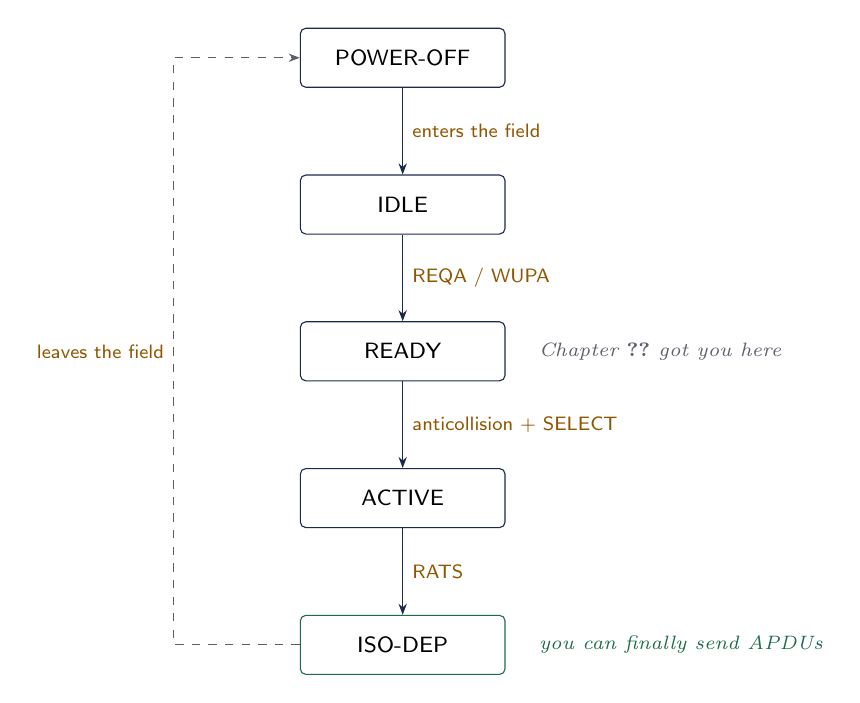
\begin{tikzpicture}[font=\footnotesize\sffamily, node distance=11mm,
   st/.style={draw=brewernavy, rounded corners=2pt, minimum width=26mm,
              minimum height=7.5mm, inner sep=3pt},
   lbl/.style={font=\scriptsize\sffamily, color=breweramber!80!black}]
  \node[st] (off) {POWER-OFF};
  \node[st, below=of off] (idle) {IDLE};
  \node[st, below=of idle] (ready) {READY};
  \node[st, below=of ready] (active) {ACTIVE};
  \node[st, below=of active, draw=brewergreen] (isodep) {ISO-DEP};
  \draw[-{Stealth[length=4pt]}, brewernavy] (off) -- node[right, lbl] {enters the field} (idle);
  \draw[-{Stealth[length=4pt]}, brewernavy] (idle) -- node[right, lbl] {REQA / WUPA} (ready);
  \draw[-{Stealth[length=4pt]}, brewernavy] (ready) -- node[right, lbl] {anticollision + SELECT} (active);
  \draw[-{Stealth[length=4pt]}, brewernavy] (active) -- node[right, lbl] {RATS} (isodep);
  \draw[-{Stealth[length=4pt]}, brewergrey, dashed]
        (isodep.west) -- ++(-16mm,0) |- node[left, lbl, pos=0.25] {leaves the field} (off.west);
  \node[font=\scriptsize\itshape, color=brewergreen, right=3mm of isodep]
       {you can finally send APDUs};
  \node[font=\scriptsize\itshape, color=brewergrey, right=3mm of ready]
       {Chapter~\ref{ch:reader} got you here};
\end{tikzpicture}
\end{center}

\section{Anticollision, and why it exists}
\index{anticollision}

Put two cards on the antenna and both answer at once --- the radio signals
collide and you get mush. ISO-14443 solves this with a bit-by-bit tree walk: the
reader asks ``everyone whose UID starts with these bits, answer'', and narrows
until exactly one card remains.

We implement the \textbf{simple case}: ask for the whole UID at once, and if the
reply's checksum is intact, exactly one card answered. If two cards collide, the
checksum fails, we return empty, and the user is told to present one card. That
is honest engineering for a coffee machine.

\paragraph{BCC.} The block check character is
\code{uid[0] \^{} uid[1] \^{} uid[2] \^{} uid[3]}. XOR the four bytes; the result
must equal the fifth. A cheap integrity check that catches both RF corruption
and undetected collisions.

\subsection{Cascade levels, and the \texttt{0x88} tag}

UIDs come in 4-byte and 7-byte flavours, but an anticollision reply is fixed at
five bytes (four data + one checksum). A 7-byte UID therefore needs two rounds:

\begin{center}
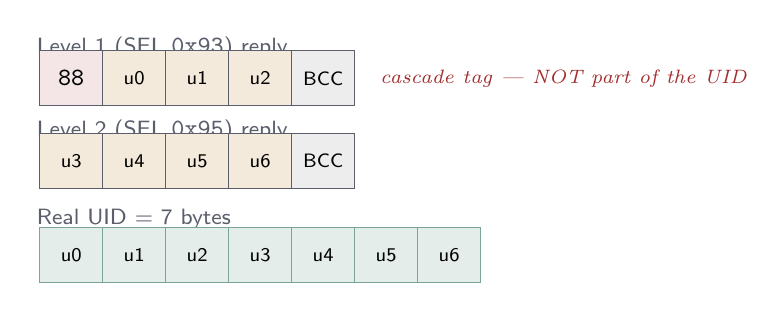
\begin{tikzpicture}[font=\scriptsize\sffamily, x=8mm, y=7mm]
  % level 1
  \node[font=\footnotesize\sffamily, anchor=west, color=brewergrey] at (-0.2,2.35)
       {Level 1 (SEL \hex{0x93}) reply};
  \foreach \i/\lbl/\c in {0/{\hex{88}}/brewerred!12, 1/{u0}/breweramber!14,
                          2/{u1}/breweramber!14, 3/{u2}/breweramber!14,
                          4/{BCC}/black!7}{
     \fill[\c] (\i,1.3) rectangle ++(1,1);
     \draw[brewergrey] (\i,1.3) rectangle ++(1,1);
     \node at (\i+0.5,1.8) {\lbl};
  }
  \node[color=brewerred, font=\scriptsize\itshape, anchor=west] at (5.25,1.8)
       {cascade tag --- NOT part of the UID};
  % level 2
  \node[font=\footnotesize\sffamily, anchor=west, color=brewergrey] at (-0.2,0.85)
       {Level 2 (SEL \hex{0x95}) reply};
  \foreach \i/\lbl in {0/{u3}, 1/{u4}, 2/{u5}, 3/{u6}}{
     \fill[breweramber!14] (\i,-0.2) rectangle ++(1,1);
     \draw[brewergrey] (\i,-0.2) rectangle ++(1,1);
     \node at (\i+0.5,0.3) {\lbl};
  }
  \fill[black!7] (4,-0.2) rectangle ++(1,1);
  \draw[brewergrey] (4,-0.2) rectangle ++(1,1);
  \node at (4.5,0.3) {BCC};
  % result
  \node[font=\footnotesize\sffamily, anchor=west, color=brewergrey] at (-0.2,-0.75)
       {Real UID = 7 bytes};
  \foreach \i/\lbl in {0/{u0}, 1/{u1}, 2/{u2}, 3/{u3}, 4/{u4}, 5/{u5}, 6/{u6}}{
     \fill[brewergreen!12] (\i,-1.9) rectangle ++(1,1);
     \draw[brewergreen!60] (\i,-1.9) rectangle ++(1,1);
     \node at (\i+0.5,-1.4) {\lbl};
  }
\end{tikzpicture}
\end{center}

The SAK from level 1 comes back with \textbf{bit 2 (\hex{0x04}) set},
confirming ``UID incomplete, do the next level''. DESFire EV2/EV3 always has a
7-byte UID, so you \emph{will} exercise this path.

\begin{trap}{Forgetting to skip the \hex{0x88}}
Keep the cascade tag and you get a 7-byte UID that is wrong in its first byte
--- and it looks completely plausible. You will only notice when it does not
match what your phone reports, which might be days later.
\end{trap}

\paragraph{RATS.} Request Answer To Select (\hex{0xE0} \hex{0x50}) is the final
handshake: ``let us speak ISO-14443-4''. The card replies with its \textbf{ATS},
describing its capabilities and maximum frame size. The \hex{0x50} parameter is
FSDI${}=5$ (we accept up to 64-byte frames) and CID${}=0$.

\section{Build it}

\subsection{\texttt{ActivatedCard} --- a value object}
\index{value object}\index{immutability}

\begin{jcode}
package com.midnightbrewer.hardware;

/**
 * What activation produced: a UID, a SAK and an ATS.
 *
 * A VALUE OBJECT -- it holds data, has no behaviour that changes it, and is
 * IMMUTABLE: every field is final and there is no setter. Once built, it can
 * never disagree with itself.
 *
 * Why bother, instead of returning byte[][] or three out-parameters?
 *   - the three fields arrive together and belong together
 *   - the compiler enforces that you cannot forget one
 *   - it has a NAME, so signatures read as intent:
 *       ActivatedCard activate()      vs      byte[][] activate()
 */
public final class ActivatedCard {

    private final byte[] uid;
    private final int sak;
    private final byte[] ats;

    public ActivatedCard(byte[] uid, int sak, byte[] ats) {
        // DEFENSIVE COPY on the way in: if we stored the caller's array
        // directly, they could mutate our state afterwards and we would
        // silently change. Copy, and we own it.
        this.uid = uid.clone();
        this.sak = sak;
        this.ats = ats.clone();
    }

    /** Defensive copy on the way OUT too, for the same reason. */
    public byte[] uid() { return uid.clone(); }

    public int sak() { return sak; }

    public byte[] ats() { return ats.clone(); }

    /** The UID as spaced uppercase hex, e.g. "04 76 18 62 7B 20 90". */
    public String uidHex() {
        // TODO: StringBuilder, String.format("%02X ", b) per byte, trim().
        return null;
    }
}
\end{jcode}

\begin{concept}{Three decisions, and why each one}
\textbf{\code{final class}} --- nobody may subclass it. For a value object that
is right: there is no such thing as a ``special kind of ActivatedCard'', and
allowing subclasses would let someone override \code{uid()} to return something
else, breaking the guarantee.

\textbf{Defensive copies both ways} --- the part people skip. Arrays in Java are
references; handing out \code{this.uid} hands out a pointer to your internals,
and the caller can scribble on it. \code{clone()} costs seven bytes and buys you
a class that genuinely cannot be corrupted from outside.

\textbf{Immutability} --- an \code{ActivatedCard} is \emph{a fact about a
moment}: ``at 14:32 this card, with this UID, was activated''. Facts do not
change. Making it immutable means you can pass it anywhere, store it, log it,
hand it to another thread, and never wonder whether something modified it.
\end{concept}

\subsection{The activation sequence}

Add these constants to \code{Iso14443Reader}:

\begin{jcode}
    /** Anticollision/SELECT command bytes for the two cascade levels. */
    private static final byte SEL_CL1 = (byte) 0x93;
    private static final byte SEL_CL2 = (byte) 0x95;

    /** NVB byte that turns an anticollision into a SELECT (full UID follows). */
    private static final byte SELECT_NVB = 0x70;

    /** SAK bit 3: "UID incomplete, do the next cascade level". */
    private static final int CASCADE_BIT = 0x04;

    /** RATS: request ISO-14443-4. PARAM 0x50 = FSDI 5, CID 0. */
    private static final byte RATS_CMD   = (byte) 0xE0;
    private static final byte RATS_PARAM = 0x50;

    /** The tag prefixing a 7-byte UID's first anticollision reply. */
    private static final byte CASCADE_TAG = (byte) 0x88;

    /** Anticollision reply is 4 UID/CT bytes + 1 BCC. */
    private static final int ANTICOLL_LENGTH = 5;
\end{jcode}

And the methods:

\begin{jcode}
    // =================================================================
    // anticollision -- ask the card for (part of) its UID.
    //
    //   C: serNum[0] = 0x93; serNum[1] = 0x20;   // 0x20 NVB = "send it all"
    //      ToCard(PCD_TRANSCEIVE, serNum, 2, ...);
    //      // verify serNum[0]^[1]^[2]^[3] == serNum[4]
    //
    // Takes selCode so it works at BOTH levels. Full bytes, so
    // bitsInLastByte = 0. Returns the 5-byte reply, or empty if invalid.
    // =================================================================
    public byte[] anticollision(byte selCode) throws SpiException {
        // TODO 1: transceive { selCode, 0x20 } with 0 bits-in-last-byte.
        // TODO 2: a valid reply is exactly ANTICOLL_LENGTH bytes; else empty.
        // TODO 3: verify the BCC (XOR of the first four == the fifth);
        //         if it fails the read was garbled -> return empty.
        // TODO 4: return the reply.
        return new byte[0];
    }

    // =================================================================
    // select -- send the UID back, receive the SAK.
    //
    //   C: buffer[0]=selCode; buffer[1]=0x70;      // 0x70 NVB = SELECT
    //      memcpy(&buffer[2], anticoll, 5);        // 4 UID + BCC
    //      CalculateCRC(buffer, 7, &buffer[7]);    // -> 9 bytes
    //      ToCard(...);   // reply = SAK(1) + CRC(2)
    //
    // @return the SAK byte, or -1 if the reply was malformed.
    // =================================================================
    public int select(byte selCode, byte[] anticoll) throws SpiException {
        // TODO 1: build a 7-byte frame { selCode, SELECT_NVB, ...anticoll(5) }.
        // TODO 2: byte[] crc = calculateCrc(frame7);
        //         build a 9-byte frame: the 7, then crc[0], crc[1].
        // TODO 3: byte[] reply = transceive(frame9, 0);
        // TODO 4: if reply.length < 1 return -1, else return reply[0] & 0xFF.
        return -1;
    }

    // =================================================================
    // rats -- ask to speak ISO-14443-4; the card returns its ATS.
    //   C: req[0]=0xE0; req[1]=0x50; CalculateCRC(req,2,&req[2]); ToCard(...)
    // =================================================================
    public byte[] rats() throws SpiException {
        // TODO: header { RATS_CMD, RATS_PARAM }, append its CRC, transceive.
        return new byte[0];
    }

    // =================================================================
    // activate() -- the whole sequence, as another TEMPLATE METHOD.
    //
    // 'final' so a subclass cannot reorder the protocol.
    //   level 1: anticollision -> select -> SAK
    //   if the SAK's cascade bit is set, the UID is 7 bytes: do level 2
    //   then RATS
    // and assembles the real UID:
    //   - 4-byte card: ac1[0..3]
    //   - 7-byte card: ac1[1..3]  (SKIP the 0x88 tag)  +  ac2[0..3]
    // =================================================================
    public final ActivatedCard activate() throws SpiException {
        // TODO 1: ac1 = anticollision(SEL_CL1); if empty -> throw SpiException.
        //         sak1 = select(SEL_CL1, ac1);
        // TODO 2: if ((sak1 & CASCADE_BIT) == 0) -> 4-byte UID:
        //         uid = ac1[0..3], return new ActivatedCard(uid, sak1, rats());
        // TODO 3: else 7-byte UID: ac2 = anticollision(SEL_CL2);
        //         sak2 = select(SEL_CL2, ac2);
        //         uid = { ac1[1], ac1[2], ac1[3], ac2[0..3] }
        //         return new ActivatedCard(uid, sak2, rats());
        return null;
    }
\end{jcode}

\section{Verify on hardware}

\begin{jcode}
if (reader.isCardPresent()) {              // wake the card into READY first
    ActivatedCard card = reader.activate();
    System.out.println("UID  = " + card.uidHex());
    System.out.printf("SAK  = 0x%02X%n", card.sak());
    System.out.println("ATS  = " + hex(card.ats()));
}
\end{jcode}

\begin{verifybox}
For a DESFire EV3:
\begin{trace}
UID  = 04 76 18 62 7B 20 90
SAK  = 0x20
ATS  = 06 75 77 81 02 80 02 F0
\end{trace}
\end{verifybox}

\paragraph{How to read that output.}

\begin{itemize}
  \item \textbf{UID starts \hex{04}} --- NXP's manufacturer byte. Seven bytes
        total, so the cascade path ran and you skipped the tag correctly.
  \item \textbf{\hex{SAK = 0x20}} --- bit 5 set means ``ISO-14443-4
        compliant''. This is the card telling you \emph{I speak APDUs}. A MIFARE
        Classic answers \hex{0x08}; if you see that, you have the wrong card and
        nothing after this chapter will work.
  \item \textbf{ATS} --- \hex{06} is its length, and the \hex{75} encodes
        FSCI${}=5$, i.e.\ a 64-byte maximum frame.
\end{itemize}

\begin{trap}{The FSCI nibble}
FSCI lives in one nibble of the ATS, and it is genuinely easy to read the wrong
one --- the original C in this project had exactly that bug.

Read the high nibble instead of the low and you conclude FSCI${}=7$, i.e.\
``128-byte frames''. You then send a 100-byte APDU, and the card silently
ignores it. Symptom: everything works until one particular command, which times
out forever.
\end{trap}

\section{Traps}

\begin{traptable}
UID is 7 bytes but wrong in byte 0 & Did not skip the \hex{0x88} cascade tag. \\
\code{select()} returns $-1$ & CRC wrong. Check \reg{ModeReg}$=$\hex{0x3D} (preset \hex{0x6363}). \\
Anticollision always returns empty & Card not in READY --- call \code{isCardPresent()} first. \\
\hex{SAK = 0x08} & It is a MIFARE Classic, not a DESFire. \\
RATS returns empty & Card does not support 14443-4, or you sent RATS twice. \\
Works, then fails on retry & Card left in ACTIVE. Power-cycle the field per transaction. \\
\end{traptable}

\section{Commit}

\begin{shell}
git add -A
git commit -m "M5: activation -- anticollision, SELECT, cascade, RATS, ActivatedCard"
\end{shell}

\chapter{The APDU channel}
\label{ch:apdu}

\chapterbrief
  {Send your first real DESFire command and get an answer.}
  {Composition and layering --- the last rung of the ladder.}
  {A real DESFire reporting its own chip type.}

\section{The problem}

The card is activated. Now you want to send it commands. Those are
\textbf{APDUs} (Application Protocol Data Units), and they need wrapping:

\begin{center}
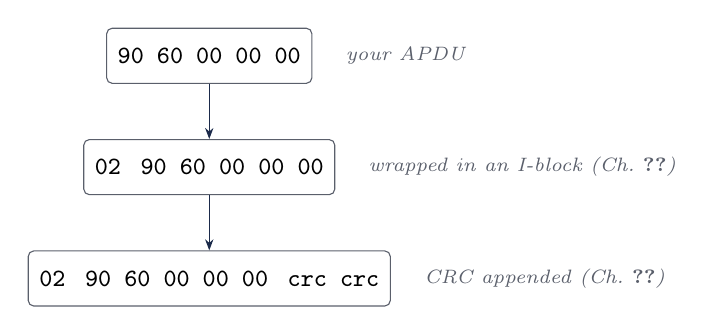
\begin{tikzpicture}[font=\footnotesize\sffamily, node distance=6mm,
   r/.style={draw=brewergrey, rounded corners=2pt, inner sep=4pt, minimum height=7mm}]
  \node[r] (a) {\code{90 60 00 00 00}};
  \node[font=\scriptsize\itshape, color=brewergrey, right=3mm of a] {your APDU};
  \node[r, below=7mm of a] (b) {\code{02} \enspace \code{90 60 00 00 00}};
  \node[font=\scriptsize\itshape, color=brewergrey, right=3mm of b]
       {wrapped in an I-block (Ch.~\ref{ch:blocks})};
  \node[r, below=7mm of b] (c) {\code{02} \enspace \code{90 60 00 00 00} \enspace \code{crc crc}};
  \node[font=\scriptsize\itshape, color=brewergrey, right=3mm of c]
       {CRC appended (Ch.~\ref{ch:reader})};
  \draw[-{Stealth[length=4pt]}, brewernavy] (a) -- (b);
  \draw[-{Stealth[length=4pt]}, brewernavy] (b) -- (c);
\end{tikzpicture}
\end{center}

Someone has to own that wrapping --- and the block-number bookkeeping that goes
with it.

\subsection{The block number: a one-bit conversation counter}

ISO-DEP puts a single bit in the I-block PCB that \textbf{alternates
0,\,1,\,0,\,1\ldots} with each exchange. It exists to disambiguate
retransmissions: if a reply is lost and you resend, the card can tell ``this is
the same command again'' from ``this is the next command''.

You must toggle it after every exchange. Get out of sync and the card ignores
you --- which looks exactly like a dead card.

\begin{concept}{State that should be impossible to get wrong}
If the block number were a parameter every caller had to pass, someone would
eventually pass the wrong one.

Hide it inside the channel as \code{private} state and toggle it automatically.
The bug becomes \emph{unrepresentable} rather than merely unlikely. That is the
strongest form of encapsulation: not ``callers should not do this'' but
``callers cannot''.
\end{concept}

\subsection{DESFire's APDU wrapping}

DESFire natively speaks its own short frames, but also accepts them wrapped in
ISO-7816 APDUs, which is what we use:

\begin{center}
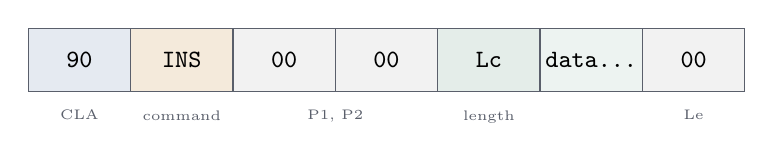
\begin{tikzpicture}[font=\scriptsize\sffamily, x=13mm, y=8mm]
  \foreach \i/\lbl/\c in {0/{\code{90}}/brewerblue!12, 1/{\code{INS}}/breweramber!14,
                          2/{\code{00}}/black!5, 3/{\code{00}}/black!5,
                          4/{\code{Lc}}/brewergreen!12, 5/{\code{data...}}/brewergreen!8,
                          6/{\code{00}}/black!5}{
     \fill[\c] (\i,0) rectangle ++(1,1);
     \draw[brewergrey] (\i,0) rectangle ++(1,1);
     \node at (\i+0.5,0.5) {\lbl};
  }
  \node[color=brewergrey, font=\tiny, anchor=north] at (0.5,-0.15) {CLA};
  \node[color=brewergrey, font=\tiny, anchor=north] at (1.5,-0.15) {command};
  \node[color=brewergrey, font=\tiny, anchor=north] at (3.0,-0.15) {P1, P2};
  \node[color=brewergrey, font=\tiny, anchor=north] at (4.5,-0.15) {length};
  \node[color=brewergrey, font=\tiny, anchor=north] at (6.5,-0.15) {Le};
\end{tikzpicture}
\end{center}

\hex{0x90} means ``DESFire native command, wrapped''. Replies end in a two-byte
status word: \hex{91 00} for OK, \hex{91 AF} for ``more frames follow'', and
various \hex{91 xx} errors. Appendix~\ref{app:vectors} lists them all.

\section{Build it}

\subsection{\texttt{ApduChannel} --- another seam}

\begin{jcode}
package com.midnightbrewer.hardware;

/**
 * "Something that can carry an APDU to a card and bring back the reply."
 *
 * The same trick as SpiLink, one layer up. The DESFire logic you write in
 * Part IV will depend only on THIS -- so it can be tested against a fake
 * channel replaying canned card replies, with no reader and no card.
 *
 * That is not a nicety. Crypto is the one thing you cannot debug by staring
 * at it, and this interface is what makes it testable offline.
 */
public interface ApduChannel {

    /** Send one APDU, return the response (including its status word). */
    byte[] transceive(byte[] apdu) throws SpiException;
}
\end{jcode}

One method. That is the whole contract, and it is enough to make all of Part~IV
testable.

\subsection{\texttt{InformationBlock.encode} --- the block gains behaviour}

Back in Chapter~\ref{ch:blocks} an I-block could only \code{describe()} itself.
Now it does real work:

\begin{jcode}
    /**
     * Encode this I-block into a frame: its PCB, then the data it carries.
     */
    public byte[] encode(byte[] inf) {
        // TODO: byte[] frame of length inf.length + 1;
        //       frame[0] = (byte) pcb();
        //       copy inf in after it; return frame.
        return null;
    }
\end{jcode}

\begin{deeper}{Designs pay off later than you would like}
The class you built two chapters ago, which looked like an academic exercise in
polymorphism, is now the thing that formats your wire frames.

That is the normal shape of good design: the structure was right before you knew
what you would need it for. It is also why ``you aren't gonna need it'' is
advice to apply to \emph{features}, not to \emph{structure}.
\end{deeper}

\subsection{\texttt{IsoDepChannel}}

\begin{jcode}
package com.midnightbrewer.hardware;

import java.util.Arrays;

/**
 * The ISO-14443-4 (ISO-DEP) channel: one APDU at a time, wrapped in an
 * I-block.
 *
 * The OOP on show:
 *   - COMPOSITION: it HAS-A reader (a channel is not a kind of reader).
 *   - ENCAPSULATED STATE: the block number toggles and nobody outside can
 *     touch it, or forget to.
 *   - it USES the Chapter 4 hierarchy: an InformationBlock encodes the frame.
 *
 * Simplifications, fine for DESFire's small frames: one I-block per APDU, no
 * chaining of large payloads, and no S-block "please wait" handling.
 */
public class IsoDepChannel implements ApduChannel {

    /** I-block PCB base; the low bit carries the block number. */
    private static final int IBLOCK_PCB = 0x02;

    private final Iso14443Reader reader;  // composition
    private int blockNumber = 0;          // private mutable state, owned here

    public IsoDepChannel(Iso14443Reader reader) {
        this.reader = reader;
    }

    /**
     *   1. wrap the APDU in an I-block for the current block number
     *   2. send it via the reader (which appends CRC and transceives)
     *   3. toggle the block number for next time
     *   4. the reply is [PCB, ...response...] -- strip the PCB
     */
    @Override
    public byte[] transceive(byte[] apdu) throws SpiException {
        // TODO 1: InformationBlock out =
        //             new InformationBlock(IBLOCK_PCB | blockNumber);
        //         byte[] frame = out.encode(apdu);
        // TODO 2: byte[] reply = reader.exchange(frame);
        // TODO 3: blockNumber ^= 1;    // toggle -- XOR with 1 flips a bit
        // TODO 4: if (reply.length < 1)
        //             throw new SpiException("empty ISO-DEP reply");
        //         return Arrays.copyOfRange(reply, 1, reply.length);
        return new byte[0];
    }
}
\end{jcode}

\subsection{\texttt{Iso14443Reader.exchange} --- the reusable primitive}

You have written ``append a CRC and transceive'' twice already, inside
\code{select()} and \code{rats()}. Pull it out:

\begin{jcode}
    // =================================================================
    // exchange() -- send a payload as a CRC-protected T=CL frame, return the
    // reply with its CRC stripped.
    //
    // The ISO-DEP channel sits on top of this: it hands us [PCB + apdu], we
    // handle the CRC and the wire.
    // =================================================================
    public byte[] exchange(byte[] payload) throws SpiException {
        // TODO 1: byte[] crc = calculateCrc(payload);
        // TODO 2: build frame = payload followed by crc[0], crc[1].
        // TODO 3: byte[] reply = transceive(frame, 0);
        // TODO 4: if (reply.length < 2) return new byte[0];
        //         return Arrays.copyOf(reply, reply.length - 2);
        return new byte[0];
    }
\end{jcode}

\section{The layer cake, complete}

You have now built six layers, each speaking only to its neighbours.

\begin{center}
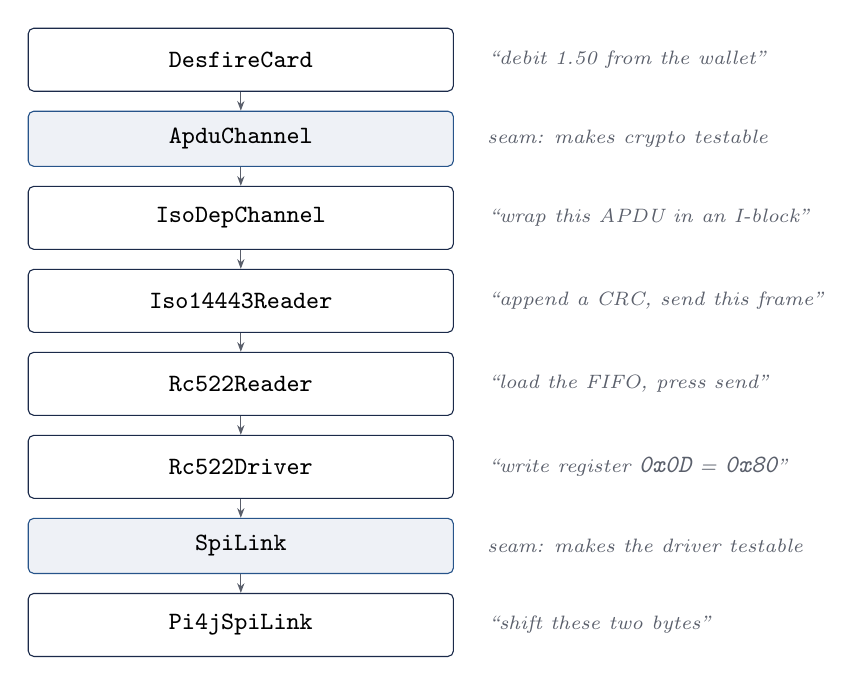
\begin{tikzpicture}[font=\footnotesize\sffamily,
  L/.style={draw=brewernavy, rounded corners=2pt, minimum width=54mm,
            minimum height=8mm, inner sep=3pt},
  S/.style={draw=brewerblue, fill=brewerblue!8, rounded corners=2pt,
            minimum width=54mm, minimum height=7mm, inner sep=3pt},
  note/.style={font=\scriptsize\itshape, color=brewergrey, anchor=west}]
  \node[L] (df) {\code{DesfireCard}};
  \node[note, right=3mm of df] {``debit 1.50 from the wallet''};
  \node[S, below=2.4mm of df] (ac) {\code{ApduChannel}};
  \node[note, right=3mm of ac] {seam: makes crypto testable};
  \node[L, below=2.4mm of ac] (idc) {\code{IsoDepChannel}};
  \node[note, right=3mm of idc] {``wrap this APDU in an I-block''};
  \node[L, below=2.4mm of idc] (ir) {\code{Iso14443Reader}};
  \node[note, right=3mm of ir] {``append a CRC, send this frame''};
  \node[L, below=2.4mm of ir] (rr) {\code{Rc522Reader}};
  \node[note, right=3mm of rr] {``load the FIFO, press send''};
  \node[L, below=2.4mm of rr] (rd) {\code{Rc522Driver}};
  \node[note, right=3mm of rd] {``write register \hex{0x0D} = \hex{0x80}''};
  \node[S, below=2.4mm of rd] (sl) {\code{SpiLink}};
  \node[note, right=3mm of sl] {seam: makes the driver testable};
  \node[L, below=2.4mm of sl] (p4) {\code{Pi4jSpiLink}};
  \node[note, right=3mm of p4] {``shift these two bytes''};
  \foreach \a/\b in {df/ac, ac/idc, idc/ir, ir/rr, rr/rd, rd/sl, sl/p4}{
     \draw[-{Stealth[length=3.5pt]}, brewergrey] (\a) -- (\b);}
\end{tikzpicture}
\end{center}

\textbf{Every arrow points down, and there are exactly two seams.} The value of
that shape: any layer can be tested by faking the layer below, and any layer can
be replaced without touching the others. Swap \code{Pi4jSpiLink} for an FT232H
and nothing above changes. Swap the RC522 for a PN532 and you write one new
\code{Iso14443Reader} subclass; nothing above changes.

\begin{concept}{What ``good architecture'' actually buys}
It is not a matter of taste. It is the property that lets you \textbf{debug one
layer at a time instead of debugging six at once.}

When something breaks in Part~IV, you will walk down this diagram asking each
layer ``are you still telling the truth?'' --- and the first \emph{no} is your
bug. Without the seams, every failure is a whole-system failure.
\end{concept}

\section{Verify --- your first conversation with a DESFire}

\begin{jcode}
IsoDepChannel channel = new IsoDepChannel(reader);
// ISO-7816-wrapped DESFire GetVersion: 90 60 00 00 00
byte[] getVersion = { (byte) 0x90, 0x60, 0x00, 0x00, 0x00 };
byte[] resp = channel.transceive(getVersion);
System.out.println("GetVersion resp = " + hex(resp));
\end{jcode}

\begin{verifybox}
\begin{trace}
GetVersion resp = 04 01 01 33 00 18 05 91 AF
\end{trace}
\end{verifybox}

Decode it --- this is your card's identity document:

\begin{center}\small
\begin{tabular}{@{}lll@{}}
\toprule
\thead{Byte} & \thead{Value} & \thead{Meaning} \\
\midrule
\hex{04}     & vendor       & NXP \\
\hex{01 01}  & type/subtype & DESFire \\
\textbf{\hex{33}} & \textbf{version} & \textbf{major 3 = EV3} (\hex{0x12} = EV1, \hex{0x22} = EV2) \\
\hex{00 18}  & storage      & \hex{0x18} $\rightarrow$ 8\,KB \\
\hex{05}     & protocol     & ISO-14443-2/3/4 \\
\hex{91 AF}  & status       & \textbf{additional frame available} \\
\bottomrule
\end{tabular}
\end{center}

\begin{trap}{\hex{91 AF} is not an error}
It is the card saying ``I have more to tell you''. \code{GetVersion} chains three
frames --- hardware info, software info, then UID and batch number. You would
send \hex{90 AF 00 00 00} twice more to drain them.

That matters practically: if you leave the card mid-chain and send a
\emph{different} command, some cards abort with an error. Either drain the chain
or power-cycle the field before the next command. This will bite you in
Chapter~\ref{ch:auth} if you do not.
\end{trap}

If the \hex{33} byte reads \hex{0x12} or \hex{0x22} you have an EV1 or EV2. EV2
works with everything in this book. \textbf{EV1 does not} --- it has no
\code{AuthenticateEV2First}, and needs the legacy \hex{0x0A}/\hex{0xAA}
authentication, which is a different algorithm.

\section{Traps}

\begin{traptable}
Empty reply & Block number out of sync, or RATS never ran. \\
Works exactly once per power-up & Not toggling the block number. \\
\hex{91 AE} on a later command & Card was mid-chain from \hex{91 AF}. \\
\hex{6E 00} / \hex{6D 00} instead of \hex{91 xx} & ISO-7816 error --- check the CLA \hex{90} and the trailing \hex{00}. \\
Reply is one byte too long & Forgot to strip the PCB. \\
\end{traptable}

\section{Commit}

\begin{shell}
git add -A
git commit -m "M6: ApduChannel seam + IsoDepChannel; GetVersion works on silicon"
\end{shell}


\part{Cryptography}
\chapter{AES-CMAC from scratch}
\label{ch:cmac}

\chapterbrief
  {Build the message authentication code DESFire EV2 runs on.}
  {Immutable objects and constructor invariants.}
  {The RFC 4493 known-answer vectors passing.}

\section{Read this before you write any cryptography}

Everything from here on is \textbf{verified against known-answer test vectors
before it touches hardware}. This is not caution for its own sake.

Cryptographic code has a property no other code you have written has:
\textbf{wrong output is indistinguishable from right output.} A broken CRC gives
you a mismatch you can see. A broken CMAC gives you sixteen bytes of
perfect-looking randomness --- exactly like a correct CMAC. You cannot eyeball
it, you cannot reason about it from a failed transaction, and if you build three
more layers before testing you will have no idea which one is lying.

On real hardware it is worse. A bad MAC does not merely fail: the card may
increment an internal error counter, and enough consecutive failures can
permanently lock a key.

\begin{center}\itshape\color{brewerred}
Vectors first. Silicon second.
\end{center}

\section{What a MAC is}

A \textbf{Message Authentication Code} answers one question: \emph{was this
message written by someone holding the secret key, and has it been altered?}

It is a keyed checksum. A CRC tells you a message survived the wire; a MAC tells
you it survived an \emph{adversary}. Without the key you cannot compute a valid
MAC, so you cannot forge or tamper.

\begin{analogy}{The wax seal}
A wax seal on a letter. Anyone can read the letter, but only the person with the
signet ring can produce the seal, and breaking it to alter the contents is
obvious.

The ring is the key; the seal is the MAC. Crucially the seal does not \emph{hide}
the letter --- MACs authenticate, they do not encrypt. Those are separate jobs,
and DESFire uses both.
\end{analogy}

\textbf{CMAC} (RFC 4493 / NIST SP 800-38B) builds a MAC out of a block cipher
you already have. Roughly: it is CBC-mode encryption where you throw away
everything except the last block. That final block depends on every bit of the
message and on the key, so it works as a fingerprint.

The subtlety CMAC adds --- and the reason it is not simply ``CBC-MAC'' --- is how
it handles the \textbf{last block}, where naive CBC-MAC has a forgery weakness.
CMAC derives two subkeys, $K_1$ and $K_2$, and XORs one of them into the final
block depending on whether the message needed padding. That is the whole trick.

\section{The algorithm}

\subsection{Part 1 --- subkey generation (RFC 4493 §2.3)}

\begin{trace}
L  = AES-ECB(K, 0^128)                 encrypt an all-zero block
K1 = L << 1;   if MSB(L)  was set:  K1 ^= Rb
K2 = K1 << 1;  if MSB(K1) was set:  K2 ^= Rb
\end{trace}

\begin{itemize}
  \item $R_b = $ \hex{0x87}, the constant from AES's finite-field polynomial.
        ``\code{\^{}= Rb}'' means XOR \emph{the last byte} with \hex{0x87}.
  \item ``MSB set'' means the top bit of the \emph{first} byte:
        \code{(x[0] \& 0x80) != 0}.
  \item \code{<< 1} shifts the whole 128-bit block left one bit --- the bit that
        falls off byte $i{+}1$'s top becomes byte $i$'s bottom.
\end{itemize}

That last one is the only fiddly part, and in C you would write it identically:

\begin{jcode}
byte[] out = new byte[16];
int carry = 0;
for (int i = 15; i >= 0; i--) {      // walk BACKWARDS, low byte first
    int b = in[i] & 0xFF;
    out[i] = (byte) ((b << 1) | carry);
    carry = (b >> 7) & 1;            // the bit shifted out of this byte
}
\end{jcode}

You walk from the last byte to the first because a carry propagates
\emph{upward}, toward the more significant end.

\subsection{Part 2 --- the MAC (RFC 4493 §2.4)}

\begin{center}
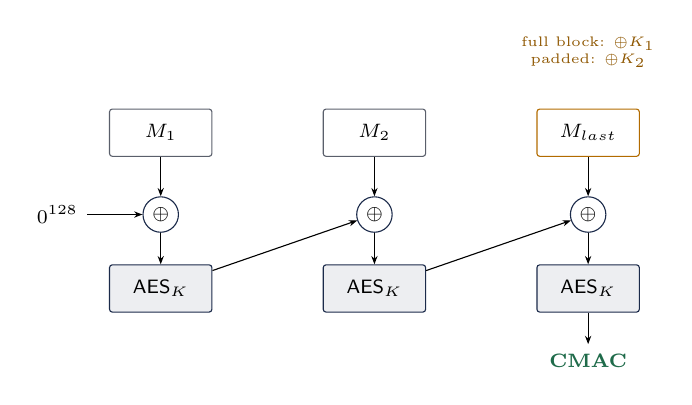
\begin{tikzpicture}[font=\scriptsize\sffamily, node distance=5mm,
  blk/.style={draw=brewergrey, rounded corners=1pt, minimum width=13mm,
              minimum height=6mm, inner sep=2pt},
  op/.style={draw=brewernavy, circle, inner sep=1pt, minimum size=4.5mm},
  aes/.style={draw=brewernavy, fill=brewernavy!8, rounded corners=1pt,
              minimum width=13mm, minimum height=6mm}]
  \node[blk] (m1) {$M_1$};
  \node[blk, right=14mm of m1] (m2) {$M_2$};
  \node[blk, right=14mm of m2, draw=breweramber] (ml) {$M_{last}$};

  \node[op, below=5mm of m1] (x1) {$\oplus$};
  \node[op, below=5mm of m2] (x2) {$\oplus$};
  \node[op, below=5mm of ml] (xl) {$\oplus$};

  \node[aes, below=4mm of x1] (a1) {AES$_K$};
  \node[aes, below=4mm of x2] (a2) {AES$_K$};
  \node[aes, below=4mm of xl] (al) {AES$_K$};

  \node[left=7mm of x1, font=\scriptsize] (zero) {$0^{128}$};

  \draw[-{Stealth[length=3pt]}] (m1) -- (x1);
  \draw[-{Stealth[length=3pt]}] (m2) -- (x2);
  \draw[-{Stealth[length=3pt]}] (ml) -- (xl);
  \draw[-{Stealth[length=3pt]}] (zero) -- (x1);
  \draw[-{Stealth[length=3pt]}] (x1) -- (a1);
  \draw[-{Stealth[length=3pt]}] (x2) -- (a2);
  \draw[-{Stealth[length=3pt]}] (xl) -- (al);
  \draw[-{Stealth[length=3pt]}] (a1) -- (x2);
  \draw[-{Stealth[length=3pt]}] (a2) -- (xl);
  \node[below=4mm of al, font=\scriptsize\bfseries, color=brewergreen] (t) {CMAC};
  \draw[-{Stealth[length=3pt]}] (al) -- (t);

  \node[above=4mm of ml, align=center, font=\tiny, color=breweramber!80!black]
       {full block: $\oplus K_1$\\ padded: $\oplus K_2$};
\end{tikzpicture}
\end{center}

\begin{trace}
split the message into 16-byte blocks M_1 ... M_n
the LAST block is special:
    if it is exactly 16 bytes:   M_last = M_n XOR K1
    otherwise (incl. empty):     pad it (append 0x80 then 0x00s to 16)
                                 M_last = padded XOR K2
then CBC-MAC:
    X = 0^128
    for each block except the last:   X = AES(K, X XOR M_i)
    T = AES(K, X XOR M_last)          <- the CMAC
\end{trace}

The $K_1$ versus $K_2$ choice is what makes ``a 16-byte message'' and ``a 15-byte
message padded to 16'' produce different MACs. Without it, an attacker could
exploit the ambiguity.

\section{Build it}

First, thin AES helpers. This is the one piece handed to you complete ---
reimplementing AES itself teaches you nothing here, and the JDK's is correct and
fast.

\begin{jcode}
package com.midnightbrewer.hardware.crypto;

import javax.crypto.Cipher;
import javax.crypto.spec.IvParameterSpec;
import javax.crypto.spec.SecretKeySpec;

/**
 * Thin AES-128 helpers over the JDK's crypto provider.
 *
 * NoPadding everywhere: DESFire does its own ISO 7816-4 padding, and letting
 * the JDK add PKCS#5 on top would corrupt every frame.
 */
public final class Aes {

    public static final int BLOCK = 16;

    private Aes() { }

    public static byte[] ecbEncrypt(byte[] key, byte[] block) {
        try {
            Cipher c = Cipher.getInstance("AES/ECB/NoPadding");
            c.init(Cipher.ENCRYPT_MODE, new SecretKeySpec(key, "AES"));
            return c.doFinal(block);
        } catch (Exception e) {
            throw new IllegalStateException("AES-ECB failed", e);
        }
    }

    public static byte[] cbcEncrypt(byte[] key, byte[] iv, byte[] data) {
        try {
            Cipher c = Cipher.getInstance("AES/CBC/NoPadding");
            c.init(Cipher.ENCRYPT_MODE, new SecretKeySpec(key, "AES"),
                   new IvParameterSpec(iv));
            return c.doFinal(data);
        } catch (Exception e) {
            throw new IllegalStateException("AES-CBC encrypt failed", e);
        }
    }

    public static byte[] cbcDecrypt(byte[] key, byte[] iv, byte[] data) {
        try {
            Cipher c = Cipher.getInstance("AES/CBC/NoPadding");
            c.init(Cipher.DECRYPT_MODE, new SecretKeySpec(key, "AES"),
                   new IvParameterSpec(iv));
            return c.doFinal(data);
        } catch (Exception e) {
            throw new IllegalStateException("AES-CBC decrypt failed", e);
        }
    }

    public static byte[] xor(byte[] a, byte[] b) {
        byte[] out = new byte[a.length];
        for (int i = 0; i < a.length; i++) {
            out[i] = (byte) (a[i] ^ b[i]);
        }
        return out;
    }
}
\end{jcode}

Now the part you write.

\begin{jcode}
package com.midnightbrewer.hardware.crypto;

/**
 * AES-CMAC (RFC 4493) -- the MAC DESFire EV2 uses. The JDK has no CMAC, so
 * this is the from-scratch part; you are not reimplementing AES, you are
 * building the CMAC construction on top of Aes.ecbEncrypt.
 *
 * OOP on show: the key and the two derived subkeys are computed ONCE in the
 * constructor and kept private. compute() never mutates them. That makes this
 * an immutable object with an invariant established at birth: "if this object
 * exists, its subkeys are correct and match its key."
 */
public final class AesCmac {

    private static final int BLOCK = 16;
    private static final byte RB = (byte) 0x87;  // AES field polynomial

    private final byte[] key;
    private final byte[] k1;
    private final byte[] k2;

    public AesCmac(byte[] key) {
        if (key.length != BLOCK) {
            throw new IllegalArgumentException("AES-128 key must be 16 bytes");
        }
        this.key = key.clone();
        byte[][] subkeys = generateSubkeys(key);
        this.k1 = subkeys[0];
        this.k2 = subkeys[1];
    }

    // ---- RFC 4493 section 2.3 ----
    private static byte[][] generateSubkeys(byte[] key) {
        // TODO 1: byte[] l = Aes.ecbEncrypt(key, new byte[BLOCK]);
        // TODO 2: byte[] k1 = leftShift(l);
        //         if ((l[0] & 0x80) != 0) k1[15] ^= RB;
        // TODO 3: byte[] k2 = leftShift(k1);
        //         if ((k1[0] & 0x80) != 0) k2[15] ^= RB;
        // TODO 4: return new byte[][]{ k1, k2 };
        return new byte[][]{ new byte[BLOCK], new byte[BLOCK] };
    }

    /** Shift a 16-byte block left by ONE bit, as a single 128-bit number. */
    private static byte[] leftShift(byte[] in) {
        // TODO: walk from the LAST byte to the first, carrying the top bit
        //       of each byte down into the next. (See the chapter text.)
        return new byte[BLOCK];
    }

    // ---- RFC 4493 section 2.4 ----
    public byte[] compute(byte[] message) {
        // TODO 1: how many blocks, and is the last one full?
        //   if (message.length == 0) { n = 1; lastComplete = false; }
        //   else { n = ceil(message.length / 16.0);
        //          lastComplete = (message.length % 16 == 0); }

        // TODO 2: build M_last.
        //   if lastComplete: mLast = Aes.xor(lastBlock, k1)
        //   else: pad into a 16-byte buffer -- copy the leftover bytes,
        //         set padded[leftoverLen] = (byte) 0x80, rest stays zero;
        //         mLast = Aes.xor(padded, k2)

        // TODO 3: CBC-MAC through the blocks:
        //   byte[] x = new byte[BLOCK];
        //   for (int i = 0; i < n - 1; i++)
        //       x = Aes.ecbEncrypt(key, Aes.xor(x, i-th 16-byte slice));
        //   return Aes.ecbEncrypt(key, Aes.xor(x, mLast));
        return new byte[BLOCK];
    }
}
\end{jcode}

\begin{concept}{Establish invariants in the constructor}
\index{invariant}
Why compute the subkeys in the constructor? Partly efficiency --- they are a pure
function of the key, and recomputing them per call would waste an AES operation
on every MAC.

But the deeper reason is \textbf{the invariant}. The constructor is the one place
that can guarantee ``this object is valid''. It checks the key length and derives
the subkeys; afterwards the object cannot be in a bad state, because nothing can
change it.

Contrast a design with a \code{setKey()} method. Now every method must ask: has
the key been set? Are the subkeys stale? Those questions do not exist if you make
them impossible.

\textbf{Establish invariants in the constructor, make fields \code{final},
expose no setters.} Half of ``good OOP'' is that one habit.
\end{concept}

\section{Verify --- RFC 4493 vectors}

These come from the RFC itself: independent of you, independent of this book,
and definitive.

\textbf{Key} $K = $ \hex{2b7e151628aed2a6abf7158809cf4f3c}

\begin{center}\small
\begin{tabular}{@{}L{0.44\linewidth}L{0.46\linewidth}@{}}
\toprule
\thead{Message} & \thead{Expected CMAC} \\
\midrule
\emph{(empty)} & \hex{bb1d6929e95937287fa37d129b756746} \\
\hex{6bc1bee22e409f96e93d7e117393172a} & \hex{070a16b46b4d4144f79bdd9dd04a287c} \\
\hex{6bc1bee22e409f96e93d7e117393172a}\newline
\hex{ae2d8a571e03ac9c9eb76fac45af8e51}\newline
\hex{30c81c46a35ce411} \emph{(40 B)} & \hex{dfa66747de9ae63030ca32611497c827} \\
the above $+$ \hex{e5fbc1191a0a52ef}\newline
\hex{f69f2445df4f9b17ad2b417be66c3710} \emph{(64 B)} & \hex{51f0bebf7e3b9d92fc49741779363cfe} \\
\bottomrule
\end{tabular}
\end{center}

Those four are chosen to hit every branch: empty (pad, $K_2$), exactly one block
($K_1$), a partial last block (pad, $K_2$), and multiple full blocks ($K_1$). If
all four pass, your implementation is right.

The subkeys, useful mid-debug:

\begin{trace}
K1 = fbeed618357133667c85e08f7236a8de
K2 = f7ddac306ae266ccf90bc11ee46d513b
\end{trace}

\begin{jcode}
package com.midnightbrewer.hardware.crypto;

import org.junit.jupiter.api.Test;
import java.util.HexFormat;
import static org.junit.jupiter.api.Assertions.assertEquals;

class AesCmacTest {

    private static final byte[] K =
            HexFormat.of().parseHex("2b7e151628aed2a6abf7158809cf4f3c");

    private static String mac(String messageHex) {
        byte[] m = HexFormat.of().parseHex(messageHex);
        return HexFormat.of().formatHex(new AesCmac(K).compute(m));
    }

    @Test
    void rfc4493_example1_empty() {
        assertEquals("bb1d6929e95937287fa37d129b756746", mac(""));
    }

    @Test
    void rfc4493_example2_oneBlock() {
        assertEquals("070a16b46b4d4144f79bdd9dd04a287c",
                mac("6bc1bee22e409f96e93d7e117393172a"));
    }

    @Test
    void rfc4493_example3_partialLastBlock() {
        assertEquals("dfa66747de9ae63030ca32611497c827",
                mac("6bc1bee22e409f96e93d7e117393172a"
                  + "ae2d8a571e03ac9c9eb76fac45af8e51"
                  + "30c81c46a35ce411"));
    }

    @Test
    void rfc4493_example4_fullBlocks() {
        assertEquals("51f0bebf7e3b9d92fc49741779363cfe",
                mac("6bc1bee22e409f96e93d7e117393172a"
                  + "ae2d8a571e03ac9c9eb76fac45af8e51"
                  + "30c81c46a35ce411e5fbc1191a0a52ef"
                  + "f69f2445df4f9b17ad2b417be66c3710"));
    }
}
\end{jcode}

\begin{verifybox}
\begin{shell}
mvn test -Dtest=AesCmacTest      # all four must be green
\end{shell}
Those four numbers were published in 2006 by people who have never seen your
code. If your code reproduces them exactly, that is not ``it seems to work'' ---
that is proof.
\end{verifybox}

\code{HexFormat} is a Java 17+ built-in, so no dependency is needed for hex
parsing and printing --- which you will do constantly from here on.

\section{Traps}

\begin{traptable}
Empty-message vector fails, others pass & Missing the \code{n=1, lastComplete=false} special case. \\
Partial-block vectors fail & Padding wrong: it is \hex{0x80} then zeros, not all zeros. \\
Full-block vectors fail & Using $K_2$ where $K_1$ belongs, or vice versa. \\
All four fail, all plausible-looking & \code{leftShift} carry direction --- you must walk backwards. \\
Sporadic wrong results & You mutated \code{key} or a subkey. They must be write-once. \\
\end{traptable}

\section{Commit}

\begin{shell}
git add -A
git commit -m "M7a: AES-CMAC (RFC 4493), verified against the RFC vectors"
\end{shell}

\chapter{Session keys}
\label{ch:sesskeys}

\chapterbrief
  {Derive the two per-transaction AES keys from the nonces exchanged during authentication.}
  {Private static helpers, and enums instead of boolean flags.}
  {EV2 key derivation verified against independent vectors.}

\section{The problem: never use the long-term key directly}

Your card holds a permanent AES-128 key. It would be technically possible to
encrypt every message with it. It would also be a bad idea, for three reasons
worth understanding:

\begin{description}[leftmargin=0pt, style=nextline]
  \item[Replay.] If one key encrypts everything forever, a recorded ``debit
        1.50'' frame stays valid. An attacker records one purchase and replays it
        --- or replays a \emph{credit}.
  \item[Traffic analysis.] The same plaintext under the same key gives the same
        ciphertext every time. An eavesdropper learns which commands are which
        without breaking anything.
  \item[Exposure.] Every message under the long-term key is another sample for
        cryptanalysis. Keys wear out with use.
\end{description}

So DESFire does what TLS does: use the long-term key \emph{once}, to bootstrap a
pair of throwaway keys valid only for this tap.

\begin{analogy}{The hotel key card}
A hotel does not hand guests the master key that opens every door forever. You
present identification at the desk once --- the long-term secret --- and they
programme a card that opens \emph{your} room, \emph{this} week. Lose it and the
damage is bounded; the master key never left the safe.

The nonces are what make each session unique. Both sides contribute randomness,
so neither can force a repeat --- which matters, because if the card alone chose,
a compromised card could replay the same session forever.
\end{analogy}

\textbf{Two keys, not one}, because encryption and authentication are different
jobs and reusing one key for both is a classic footgun:

\begin{itemize}
  \item $K_{enc}$ --- encrypts data. \emph{Confidentiality}: nobody can read the balance.
  \item $K_{mac}$ --- authenticates commands. \emph{Integrity}: nobody can alter the debit.
\end{itemize}

\section{The derivation}

Both keys come from the same construction with a different label byte. The input
is a 32-byte ``session vector'' (SV):

\begin{center}
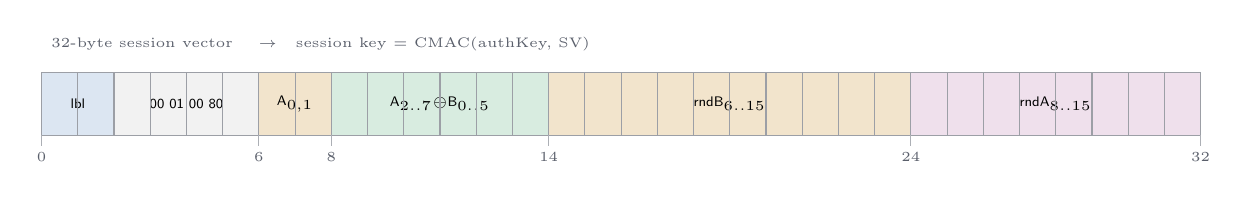
\begin{tikzpicture}[font=\scriptsize\sffamily, x=4.6mm, y=8mm]
  \definecolor{c1}{HTML}{DCE6F2}
  \definecolor{c2}{HTML}{F2E4CC}
  \definecolor{c3}{HTML}{D8ECE0}
  \definecolor{c4}{HTML}{EFE0EC}
  % row of 32 cells
  \foreach \i in {0,...,31}{ \draw[brewergrey!60] (\i,0) rectangle ++(1,1); }
  \fill[c1] (0,0) rectangle (2,1);   \node at (1,0.5) {\tiny lbl};
  \fill[black!5] (2,0) rectangle (6,1); \node at (4,0.5) {\tiny 00 01 00 80};
  \fill[c2] (6,0) rectangle (8,1);   \node at (7,0.5) {\tiny A$_{0,1}$};
  \fill[c3] (8,0) rectangle (14,1);  \node at (11,0.5) {\tiny A$_{2..7}\oplus$B$_{0..5}$};
  \fill[c2] (14,0) rectangle (24,1); \node at (19,0.5) {\tiny rndB$_{6..15}$};
  \fill[c4] (24,0) rectangle (32,1); \node at (28,0.5) {\tiny rndA$_{8..15}$};
  \foreach \i in {0,...,31}{ \draw[brewergrey!60] (\i,0) rectangle ++(1,1); }
  % byte index ruler
  \foreach \i/\lbl in {0/0, 6/6, 8/8, 14/14, 24/24, 32/32}{
     \node[color=brewergrey, font=\tiny] at (\i,-0.35) {\lbl};
     \draw[brewergrey!50] (\i,0) -- (\i,-0.18);
  }
  \node[color=brewergrey, font=\tiny, anchor=west] at (0,1.45)
       {32-byte session vector \quad$\rightarrow$\quad session key $=$ CMAC(authKey, SV)};
\end{tikzpicture}
\end{center}

\begin{trace}
SV[0]      label            0xA5 for Kenc, 0x5A for Kmac
SV[1]      counter-label    the other one (0x5A when label is 0xA5)
SV[2..5]   00 01 00 80      fixed
SV[6..7]   rndA[0..1]
SV[8..13]  rndA[2..7] XOR rndB[0..5]      <- the interleave
SV[14..23] rndB[6..15]
SV[24..31] rndA[8..15]

session key = CMAC(authKey, SV)           32 bytes in, 16 out
\end{trace}

The CMAC you built in Chapter~\ref{ch:cmac} is doing duty here as a \textbf{key
derivation function}: it mixes a lot of input down into sixteen bytes in a way
that cannot be inverted. That is the same property that makes it a good MAC.

\begin{deeper}{Why the strange interleave?}
Both sides must derive identical keys, so the layout is ultimately just a
specification both implement. But note \emph{why it is mixed rather than
concatenated}: bytes from both nonces are XOR'd together, so neither party can
steer the result by choosing their nonce cleverly.

If the layout were plain \code{rndA || rndB}, a malicious reader could pick
\code{rndA} to force structure into the derived key. The interleave denies both
sides that control.

And \hex{0xA5}/\hex{0x5A} are bit-complements of each other, chosen to be
maximally distinct so the two derivations cannot accidentally collide. The label
sits at byte 0, so the very first AES block of the CMAC already differs and the
two computations diverge immediately.
\end{deeper}

\section{Build it}

\begin{jcode}
package com.midnightbrewer.hardware.crypto;

import java.util.Arrays;

/**
 * One authenticated session with a card: the two derived keys, and (from
 * Chapter 10) the secure-messaging state that goes with them.
 *
 * The keys are derived ONCE in the constructor and never change -- the same
 * invariant discipline as AesCmac. If a DesfireSession exists, its keys are
 * valid and belong together.
 */
public class DesfireSession {

    private final byte[] keyEnc;
    private final byte[] keyMac;

    /**
     * Which key we are deriving.
     *
     * An ENUM, not a boolean. deriveSessionKey(key, a, b, true) at a call site
     * tells you nothing -- true what? SessionKeyType.ENC is self-documenting,
     * the compiler rejects anything else, and adding a third key type later
     * does not change any existing signature.
     */
    private enum SessionKeyType { ENC, MAC }

    public DesfireSession(byte[] authKey, byte[] rndA, byte[] rndB) {
        if (authKey.length != 16) {
            throw new IllegalArgumentException("auth key must be 16 bytes");
        }
        this.keyEnc = deriveSessionKey(authKey, rndA, rndB, SessionKeyType.ENC);
        this.keyMac = deriveSessionKey(authKey, rndA, rndB, SessionKeyType.MAC);
    }

    // =================================================================
    // private static: it is a pure function (same inputs -> same output,
    // touches no instance state), so it does not need 'this'. Marking it
    // static says exactly that, and lets the constructor call it before the
    // object is finished being built.
    // =================================================================
    private static byte[] deriveSessionKey(byte[] authKey, byte[] rndA,
                                           byte[] rndB, SessionKeyType type) {
        if (rndA.length != 16 || rndB.length != 16) {
            throw new IllegalArgumentException("nonces must be 16 bytes");
        }
        byte[] sv = new byte[32];

        // TODO 1: sv[0] = 0xA5 for ENC, 0x5A for MAC.
        //         sv[1] = the opposite one.
        // TODO 2: sv[2..5] = 0x00, 0x01, 0x00, 0x80
        // TODO 3: sv[6] = rndA[0];  sv[7] = rndA[1];
        // TODO 4: sv[8..13] = rndA[2..7] XOR rndB[0..5]
        //         (Arrays.copyOfRange + Aes.xor is the tidy way)
        // TODO 5: sv[14..23] = rndB[6..15]     (10 bytes)
        // TODO 6: sv[24..31] = rndA[8..15]     (8 bytes)
        // TODO 7: return new AesCmac(authKey).compute(sv);
        return new byte[16];
    }

    /** Defensive copies -- callers must not be able to scribble on our keys. */
    public byte[] encKey() { return keyEnc.clone(); }

    public byte[] macKey() { return keyMac.clone(); }
}
\end{jcode}

\section{Two design notes worth absorbing}

\subsection{Enum over boolean}
\index{enum}

Compare these call sites:

\begin{jcode}
deriveSessionKey(key, rndA, rndB, true);                 // true... what?
deriveSessionKey(key, rndA, rndB, SessionKeyType.ENC);   // obvious
\end{jcode}

A boolean parameter is a note-to-self that the reader does not get to see. This
is sometimes called the \textbf{boolean trap}. Any time you are about to add a
\code{boolean} parameter that selects \emph{behaviour} rather than expressing
\emph{a yes/no fact}, an enum is better: self-documenting at the call site,
extensible without changing signatures, and impossible to pass the wrong way
round.

\subsection{Do not keep scratch work as state}

A tempting first draft stores the SV and the derived key as fields:

\begin{jcode}
private byte[] SV;      // don't
private byte[] SK;      // don't
\end{jcode}

Now the object has fields that are only meaningful \emph{during} construction.
Anyone reading the class must work out whether they are still valid later, and a
second call to a derive method would silently clobber them.

\begin{concept}{Fields versus locals}
\textbf{Scratch work belongs in local variables. Fields are for state the object
genuinely \emph{has}.}

\code{keyEnc} and \code{keyMac} are state. \code{sv} is a temporary. The test:
\emph{``if someone asked this object about this field a minute from now, would
the answer be meaningful?''} If not, it is a local.
\end{concept}

\section{Verify}

These vectors were generated independently with Python's \code{cryptography}
library, so agreement means your Java is \emph{right} --- not merely
self-consistent.

\begin{trace}
authKey = 00112233445566778899aabbccddeeff
rndA    = a0a1a2a3a4a5a6a7a8a9aaabacadaeaf
rndB    = b0b1b2b3b4b5b6b7b8b9babbbcbdbebf

-> Kenc  = d46c03528ecd3b1f1148e708d3e9729d
-> Kmac  = 116d156cc502da820eb57915f189ec74
\end{trace}

\begin{jcode}
package com.midnightbrewer.hardware.crypto;

import org.junit.jupiter.api.Test;
import java.util.HexFormat;
import static org.junit.jupiter.api.Assertions.assertEquals;

class DesfireSessionTest {

    @Test
    void derivesBothSessionKeys() {
        byte[] authKey = HexFormat.of()
                .parseHex("00112233445566778899aabbccddeeff");
        byte[] rndA = HexFormat.of()
                .parseHex("a0a1a2a3a4a5a6a7a8a9aaabacadaeaf");
        byte[] rndB = HexFormat.of()
                .parseHex("b0b1b2b3b4b5b6b7b8b9babbbcbdbebf");

        DesfireSession session = new DesfireSession(authKey, rndA, rndB);

        assertEquals("d46c03528ecd3b1f1148e708d3e9729d",
                HexFormat.of().formatHex(session.encKey()));
        assertEquals("116d156cc502da820eb57915f189ec74",
                HexFormat.of().formatHex(session.macKey()));
    }
}
\end{jcode}

\begin{verifybox}
\begin{shell}
mvn test -Dtest=DesfireSessionTest
\end{shell}
\textbf{If only one key is wrong}, your \code{sv[0]}/\code{sv[1]} labels are
swapped. \textbf{If both are wrong}, the SV layout is off --- print your \code{sv}
as hex and compare byte-by-byte against the diagram. The first eight bytes should
read \hex{a5 5a 00 01 00 80 a0 a1}, and eyeballing those finds most mistakes in
seconds.
\end{verifybox}

\section{Traps}

\begin{traptable}
Both keys wrong & SV layout. Print it and compare against the spec. \\
Keys swapped & Label bytes \hex{0xA5}/\hex{0x5A} reversed. \\
\code{ArrayIndexOutOfBounds} in the XOR & Slice lengths: \code{rndA[2..7]} is 6 bytes, \code{rndB[6..15]} is 10, \code{rndA[8..15]} is 8. \\
Works in the test, fails on the card & You passed \code{rndB} where \code{rndA} belongs. The order matters. \\
\end{traptable}

\section{Commit}

\begin{shell}
git add -A
git commit -m "M7b: EV2 session key derivation, verified against independent vectors"
\end{shell}

\chapter{Mutual authentication}
\label{ch:auth}

\chapterbrief
  {Prove to the card you hold its key, make it prove the same to you, and establish a session --- without either side ever transmitting the key.}
  {Injecting randomness as a seam.}
  {A real card cryptographically proving it holds your key.}

\section{The problem}

You and the card both --- allegedly --- hold the same sixteen-byte AES key. How
do you each verify that about the other, over a radio link anyone can listen to,
without sending the key?

You cannot send it. You cannot send a hash of it, because an eavesdropper simply
replays the hash. You need each side to demonstrate \emph{use} of the key on
something new every time.

\section{The idea: challenge--response, in both directions}

I send you a random number and ask you to encrypt it. Only someone with the key
can produce the right answer. Because the number is new each time, a recorded
answer is worthless later.

Do it in both directions and you have \textbf{mutual} authentication.

\begin{analogy}{Two spies meeting}
One says ``the nightingale sings at midnight'' --- a line only someone briefed
would recognise.

If only \emph{one} side gives a passphrase, an impostor can collect it and use it
elsewhere. Both sides challenging each other means neither can be impersonated.

The rotation below is the detail that makes it work: you do not send back
\emph{the number you were given}, you send back a \textbf{transformation} of it,
proving you actually decrypted and processed it rather than echoing bytes.
\end{analogy}

\section{The dance}

\begin{center}
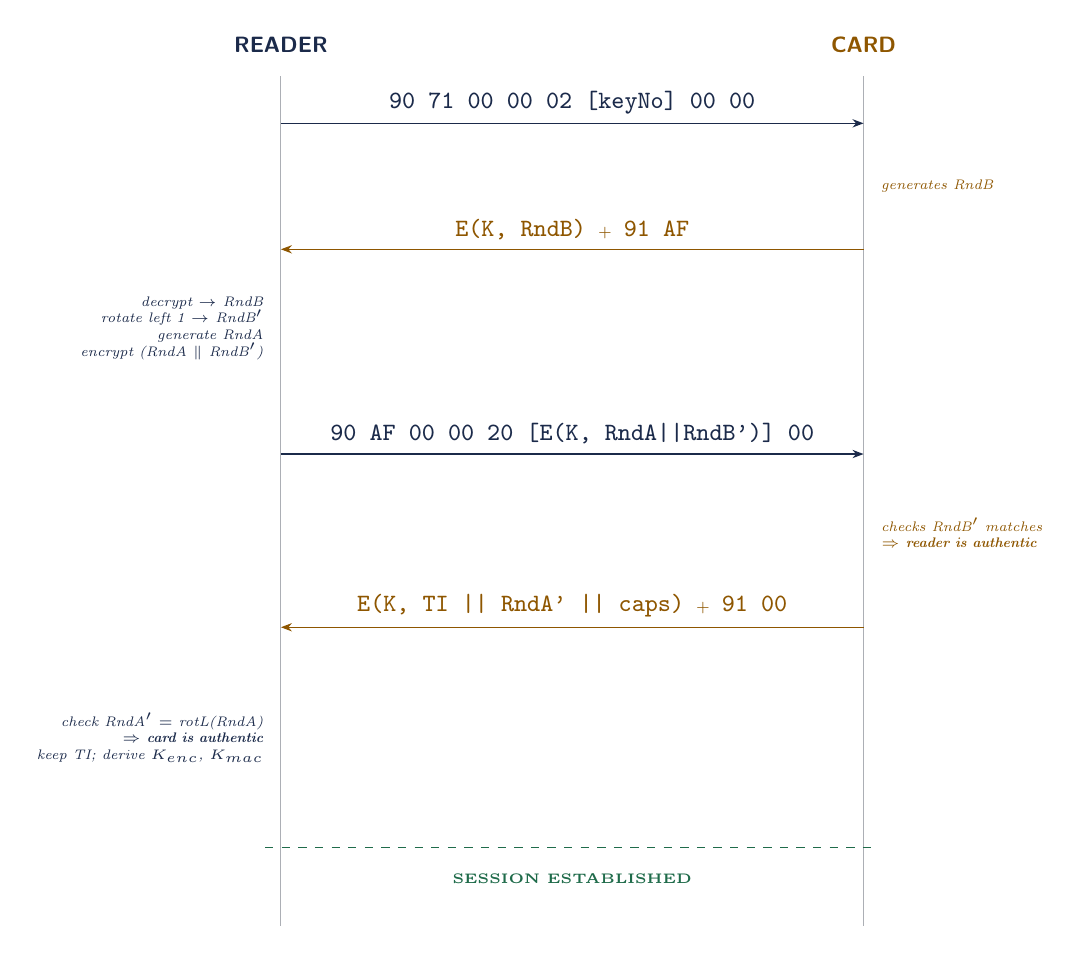
\begin{tikzpicture}[font=\scriptsize\sffamily, x=1mm, y=1mm]
  \def\L{0}   \def\R{74}
  % lifelines
  \node[font=\footnotesize\sffamily\bfseries, color=brewernavy] at (\L,4) {READER};
  \node[font=\footnotesize\sffamily\bfseries, color=breweramber!80!black] at (\R,4) {CARD};
  \draw[brewergrey!50] (\L,0) -- (\L,-108);
  \draw[brewergrey!50] (\R,0) -- (\R,-108);

  % msg 1
  \draw[-{Stealth[length=4pt]}, brewernavy] (\L,-6) -- node[above, font=\tiny] {\code{90 71 00 00 02 [keyNo] 00 00}} (\R,-6);
  \node[right=1mm of {(\R,-14)}, anchor=west, font=\tiny\itshape, color=breweramber!80!black, align=left]
       {generates RndB};
  % msg 2
  \draw[-{Stealth[length=4pt]}, breweramber!80!black] (\R,-22) -- node[above, font=\tiny] {\code{E(K, RndB)} \;+\; \hex{91 AF}} (\L,-22);

  \node[left=1mm of {(\L,-32)}, anchor=east, font=\tiny\itshape, color=brewernavy, align=right]
       {decrypt $\rightarrow$ RndB\\ rotate left 1 $\rightarrow$ RndB$'$\\ generate RndA\\ encrypt (RndA $\|$ RndB$'$)};

  % msg 3
  \draw[-{Stealth[length=4pt]}, brewernavy] (\L,-48) -- node[above, font=\tiny] {\code{90 AF 00 00 20 [E(K, RndA||RndB')] 00}} (\R,-48);
  \node[right=1mm of {(\R,-58)}, anchor=west, font=\tiny\itshape, color=breweramber!80!black, align=left]
       {checks RndB$'$ matches\\ $\Rightarrow$ \textbf{reader is authentic}};
  % msg 4
  \draw[-{Stealth[length=4pt]}, breweramber!80!black] (\R,-70) -- node[above, font=\tiny] {\code{E(K, TI || RndA' || caps)} \;+\; \hex{91 00}} (\L,-70);

  \node[left=1mm of {(\L,-84)}, anchor=east, font=\tiny\itshape, color=brewernavy, align=right]
       {check RndA$'$ $=$ rotL(RndA)\\ $\Rightarrow$ \textbf{card is authentic}\\ keep TI; derive $K_{enc}$, $K_{mac}$};

  \draw[brewergreen, dashed] (\L-2,-98) -- (\R+2,-98);
  \node[font=\tiny\bfseries, color=brewergreen] at (37,-102) {SESSION ESTABLISHED};
\end{tikzpicture}
\end{center}

\begin{trap}{Every AES operation here uses an all-zero IV}
Every single one. That is unusual --- normally a fixed IV is a flaw --- and it is
safe \emph{only} because every plaintext contains fresh randomness.

Do not carry the habit anywhere else. In Chapter~\ref{ch:secmsg} the IVs are
derived per command, precisely because the plaintexts there are predictable.
\end{trap}

\paragraph{Rotate left by one byte} means \code{b[1], b[2], ... b[15], b[0]} ---
a \emph{byte} rotation, not a bit rotation:

\begin{trace}
rotateLeft(b0b1b2b3b4b5b6b7b8b9babbbcbdbebf)
         = b1b2b3b4b5b6b7b8b9babbbcbdbebfb0
\end{trace}

\paragraph{TI}, the Transaction Identifier, is four bytes the card generates
fresh for this session. From Chapter~\ref{ch:secmsg} on, it goes into every MAC
and every IV, binding all subsequent traffic to \emph{this} authentication. It is
the session's fingerprint.

\subsection{The step-2 reply, byte by byte}

The card returns 32 encrypted bytes; decrypted they are:

\begin{center}\small
\begin{tabular}{@{}lll@{}}
\toprule
\thead{Offset} & \thead{Size} & \thead{Contents} \\
\midrule
\code{[0..4)}   & 4  & TI --- the transaction identifier \\
\code{[4..20)}  & 16 & RndA$'$ --- your RndA, rotated left \\
\code{[20..26)} & 6  & PDcap2 --- card capabilities \\
\code{[26..32)} & 6  & PCDcap2 --- reader capabilities echoed back \\
\bottomrule
\end{tabular}
\end{center}

You need the first two. The capabilities you can ignore.

\section{The testability problem, and the seam that solves it}

Here is a genuine engineering puzzle. This function calls a random number
generator, so it \textbf{produces different output every run}. How do you write a
known-answer test for it?

The answer is the same move as Chapter~\ref{ch:spi}: \textbf{the thing that
varies becomes a parameter.} Randomness is a dependency like any other. Inject
it, and a test can inject a \emph{fixed} ``random'' number, making the whole
handshake deterministic and checkable.

\begin{jcode}
package com.midnightbrewer.hardware;

import java.security.SecureRandom;

/**
 * A source of random bytes -- the seam that makes the auth handshake testable.
 *
 * Production uses secure(). A test injects a fake returning a FIXED RndA, and
 * suddenly the whole handshake is a known-answer test.
 *
 * @FunctionalInterface = exactly one abstract method, so a fake can be written
 * as a one-line lambda:   RandomSource fixed = n -> myFixedBytes;
 */
@FunctionalInterface
public interface RandomSource {

    byte[] nextBytes(int n);

    /** The real one, backed by a cryptographically secure RNG. */
    static RandomSource secure() {
        SecureRandom rng = new SecureRandom();
        return n -> {
            byte[] out = new byte[n];
            rng.nextBytes(out);
            return out;
        };
    }
}
\end{jcode}

\begin{trap}{\texttt{SecureRandom}, never \texttt{java.util.Random}}
\code{Random} is a linear congruential generator: observe a couple of outputs and
you can predict every future one. For a nonce, that is the entire security of the
protocol.

\code{SecureRandom} draws from the operating system's entropy pool. This is a
one-word difference with a catastrophic failure mode, and it is exactly the kind
of thing that ships.
\end{trap}

\begin{concept}{A seam is not a licence}
The \code{RandomSource} seam exists so \emph{tests} can pin randomness. If
production code ever passes anything but \code{RandomSource.secure()}, the
protocol is broken.

Test doubles live in \code{src/test} and that is not an accident: the build
system enforces that a fixed-nonce implementation cannot reach the kiosk.
\end{concept}

\section{Build it}

\begin{jcode}
package com.midnightbrewer.hardware;

import com.midnightbrewer.hardware.crypto.Aes;
import com.midnightbrewer.hardware.crypto.DesfireSession;
import java.util.Arrays;

/**
 * A DESFire card, spoken to over an ApduChannel.
 *
 * COMPOSITION: it HAS-A channel and HAS-A random source, both injected. It
 * knows nothing about SPI, the RC522, or ISO-DEP framing -- only APDUs in and
 * responses out. That is why it can be tested with no hardware at all.
 */
public class DesfireCard {

    private final ApduChannel channel;
    private final RandomSource randomSource;

    private byte[] ti;                 // transaction identifier, set at auth
    private DesfireSession session;    // the derived keys, set at auth

    public DesfireCard(ApduChannel channel, RandomSource randomSource) {
        this.channel = channel;
        this.randomSource = randomSource;
    }

    /**
     * Wrap a DESFire command in an ISO-7816 APDU and send it.
     *   90 [cmd] 00 00 [Lc] [data...] 00
     */
    private byte[] wrapApdu(byte cmd, byte[] data) throws SpiException {
        byte[] apdu = new byte[data.length + 6];
        apdu[0] = (byte) 0x90;              // CLA: DESFire native, wrapped
        apdu[1] = cmd;                      // INS
        apdu[2] = 0x00;                     // P1
        apdu[3] = 0x00;                     // P2
        apdu[4] = (byte) data.length;       // Lc
        System.arraycopy(data, 0, apdu, 5, data.length);
        apdu[apdu.length - 1] = 0x00;       // Le
        return channel.transceive(apdu);
    }

    /** Rotate left by one BYTE: b[1..n-1] followed by b[0]. */
    private static byte[] rotateLeft(byte[] array) {
        // TODO
        return array;
    }

    /** SelectApplication (0x5A). The AID goes on the wire LSB-first. */
    public void selectApplication(byte[] aid) throws SpiException {
        if (aid.length != 3) {
            throw new IllegalArgumentException("AID must be 3 bytes");
        }
        byte[] response = wrapApdu((byte) 0x5A, aid);
        if (response.length < 2) {
            throw new SpiException("SelectApplication failed");
        }
    }

    // =================================================================
    // AuthenticateEV2First (0x71). All AES here uses an ALL-ZERO IV.
    // =================================================================
    public void authenticateEv2First(byte keyNo, byte[] key) throws SpiException {
        if (key.length != 16) {
            throw new IllegalArgumentException("key must be 16 bytes");
        }

        // ---- step 1: ask for the challenge ----
        // TODO 1: byte[] r1 = wrapApdu((byte) 0x71, new byte[]{ keyNo, 0x00 });
        //
        //   TWO data bytes: the key number AND a 0x00 "length of capabilities"
        //   byte. Sending only keyNo gets you 91 7E (length error) and it is a
        //   genuinely annoying hour to find.
        //
        // TODO 2: strip the 2 status bytes -> encRndB (16 bytes)
        // TODO 3: byte[] rndB = Aes.cbcDecrypt(key, new byte[16], encRndB);

        // ---- step 2: answer, and challenge back ----
        // TODO 4: byte[] rndBRot = rotateLeft(rndB);
        //         byte[] rndA    = randomSource.nextBytes(16);
        // TODO 5: build a 32-byte buffer: rndA then rndBRot.
        //         byte[] encAB = Aes.cbcEncrypt(key, new byte[16], that);
        //
        //   ONE 32-byte CBC run, not two 16-byte ones. In CBC the second block
        //   chains off the first's ciphertext -- encrypting them separately
        //   gives a different, wrong answer.
        //
        // TODO 6: byte[] r2 = wrapApdu((byte) 0xAF, encAB);
        //         strip the status bytes -> encResp (32 bytes)

        // ---- step 3: verify the card, keep the session ----
        // TODO 7: byte[] plain = Aes.cbcDecrypt(key, new byte[16], encResp);
        // TODO 8: byte[] rndARot = Arrays.copyOfRange(plain, 4, 20);
        //         if (!Arrays.equals(rndARot, rotateLeft(rndA)))
        //             throw new SpiException("authentication failed: RndA mismatch");
        //
        //   THIS CHECK IS THE WHOLE POINT. Skip it and you have not
        //   authenticated the card -- you have merely talked to something.
        //
        // TODO 9: this.ti = Arrays.copyOfRange(plain, 0, 4);
        //         this.session = new DesfireSession(key, rndA, rndB);
    }

    public byte[] getTi() { return ti; }
}
\end{jcode}

\section{Verify --- the full handshake, offline}

The elegant part: your test class can \textbf{be} the fake card and the fake
random source at once.

\begin{jcode}
package com.midnightbrewer.hardware;

import java.util.Arrays;
import java.util.HexFormat;
import org.junit.jupiter.api.Test;
import static org.junit.jupiter.api.Assertions.assertArrayEquals;

/**
 * The test IS its own fake card + fake RNG: it implements both seams, so
 * new DesfireCard(this, this) plugs the test straight into the card.
 */
public class DesfireCardTest implements RandomSource, ApduChannel {

    byte[] key   = HexFormat.of().parseHex("00112233445566778899aabbccddeeff");
    byte[] rndA  = HexFormat.of().parseHex("a0a1a2a3a4a5a6a7a8a9aaabacadaeaf");
    byte[] encAB = HexFormat.of().parseHex(
            "cf086a82c0b745a749daabb28a7a8db3"
          + "32272f9e5fdc37a4746064f25b7c2ca7");
    byte[] tiExpected = HexFormat.of().parseHex("11223344");

    // Replies MUST carry the trailing status word -- the card code strips the
    // last two bytes off every reply. Without them you chop real ciphertext
    // and decrypt garbage.
    byte[] selectReply = HexFormat.of().parseHex("9100");
    byte[] step1Reply  = HexFormat.of().parseHex(
            "eab6822fe368d5bc9895fb2558b38dde" + "91af");
    byte[] step2Reply  = HexFormat.of().parseHex(
            "4e08e447d74810052caa1c5b6c60343f"
          + "51f6e901ad171e677b100d3a34c925e4" + "9100");

    @Override
    public byte[] nextBytes(int n) {
        return rndA;                        // pin RndA -> deterministic
    }

    @Override
    public byte[] transceive(byte[] apdu) throws SpiException {
        switch (apdu[1]) {                  // dispatch on INS
            case (byte) 0x5A:
                return selectReply;
            case (byte) 0x71:
                return step1Reply;
            case (byte) 0xAF:
                // assert on what we SENT: encAB sits at [5 .. len-1)
                assertArrayEquals(encAB,
                        Arrays.copyOfRange(apdu, 5, apdu.length - 1),
                        "step-2 ciphertext is wrong");
                return step2Reply;
            default:
                throw new SpiException("unexpected APDU");
        }
    }

    @Test
    public void authenticateEv2First_matchesReplayVectors() throws SpiException {
        DesfireCard card = new DesfireCard(this, this);

        card.selectApplication(new byte[]{ 0x01, 0x02, 0x03 });
        card.authenticateEv2First((byte) 0x00, key);  // no throw == RndA' verified

        assertArrayEquals(tiExpected, card.getTi());
    }
}
\end{jcode}

\begin{concept}{Why this test is strong}
It checks \emph{both} directions:

\begin{itemize}
  \item the \hex{0xAF} case asserts the exact ciphertext \textbf{you sent} ---
        proving your rotate, your concatenation and your CBC encryption are all
        correct;
  \item reaching the end without throwing proves your RndA$'$ verification passed;
  \item the TI assertion proves you sliced the reply correctly.
\end{itemize}

A test that only checked the return value would pass even if you had skipped the
RndA$'$ comparison entirely.
\end{concept}

\begin{verifybox}
\begin{shell}
mvn test -Dtest=DesfireCardTest
\end{shell}
The full vector set is in Appendix~\ref{app:vectors}.
\end{verifybox}

\section{Then: on the real card}

\begin{jcode}
DesfireCard desfire = new DesfireCard(channel, RandomSource.secure());
desfire.selectApplication(new byte[]{ 0x03, 0x02, 0x01 });  // AID 0x010203, LSB-first
byte[] appKey = new byte[16];
Arrays.fill(appKey, (byte) 0x22);                           // your app's user key
desfire.authenticateEv2First((byte) 0x02, appKey);          // key slot 2
System.out.println("MUTUAL AUTH OK. TI = " + hex(desfire.getTi()));
\end{jcode}

\begin{verifybox}
\begin{trace}
MUTUAL AUTH OK. TI = 8071F582
\end{trace}
Run it twice. \textbf{The TI will be different every time} --- it is freshly
generated per session. Seeing it change is your proof that this was a live
authentication and not a replay of your test vectors.
\end{verifybox}

\begin{trap}{A factory-blank card will fail here}
Its default master key is DES, not AES, and there is no application yet. The card
must be personalised first --- that is Chapter~\ref{ch:android}'s job.

If you do not have a provisioned card, use the top-up app's setup screen before
attempting this chapter on hardware.
\end{trap}

\section{Traps}

\begin{traptable}
\hex{91 7E} (length error) on step 1 & Sent only \code{keyNo}. It must be \code{\{ keyNo, 0x00 \}}. \\
\hex{91 AE} (auth error) on step 2 & Wrong key, wrong key number, or wrong application selected. \\
RndA mismatch but vectors pass & Check you rotated \emph{left}, and by a byte not a bit. \\
Test decrypts garbage & Fake replies missing their \hex{91 xx} status word. \\
Ciphertext differs from the vector & You encrypted RndA and RndB$'$ as two separate CBC calls. \\
Auth ``succeeds'' always & You skipped the RndA$'$ comparison. Verify you actually throw. \\
\end{traptable}

\section{Commit}

\begin{shell}
git add -A
git commit -m "M7c: AuthenticateEV2First, verified offline against replay vectors"
\end{shell}

\chapter{Secure messaging and the debit}
\label{ch:secmsg}

\chapterbrief
  {Read the balance and spend money.}
  {Growing a class as its responsibilities grow.}
  {\textbf{Money moving off a real card.}}

\section{The problem}

You are authenticated. But the card will no longer accept a bare command --- each
one must now prove three things:

\begin{enumerate}
  \item \textbf{Authenticity} --- an 8-byte CMAC computed with $K_{mac}$.
  \item \textbf{Freshness} --- a command counter, so no frame can be replayed.
  \item \textbf{Confidentiality} (for values) --- the amount encrypted with $K_{enc}$.
\end{enumerate}

That is ``CommMode.Full'', and it is what a value file configured for full
protection demands.

\begin{analogy}{The cheque}
The \textbf{amount} is written in the box --- the encrypted data. The
\textbf{signature} proves you authorised it --- the MAC. And the \textbf{cheque
number} stops the payee photocopying it and cashing it twice --- the counter.

Remove any one and the system fails: no signature, anyone writes cheques; no
number, one cheque pays forever; no amount protection, someone alters 10 to 1000.
\end{analogy}

\section{The command counter, and the ordering that will bite you}

\code{CmdCtr} is a 16-bit counter that starts at \textbf{0} immediately after
authentication and increments by one per accepted command. It goes into every MAC
and every IV, so no two commands in a session look alike.

Here is the rule that costs people an evening:

\begin{center}
\begin{tikzpicture}[font=\scriptsize\sffamily, x=1mm, y=1mm]
  \draw[brewergrey!60, -{Stealth[length=4pt]}] (0,0) -- (108,0);
  \foreach \x/\lbl in {6/{\code{ctr = 0}}, 58/{\code{ctr = 1}}}{
     \node[font=\scriptsize\sffamily\bfseries, color=brewernavy, anchor=west] at (\x,7) {\lbl};}
  % events
  \foreach \x/\lbl/\c in {
      8/{build command MAC}/brewernavy,
      30/{send}/brewergrey,
      48/{card accepts}/breweramber!80!black,
      62/{\textbf{increment}}/brewerred,
      80/{verify response MAC}/brewergreen,
      96/{decrypt response}/brewergreen}{
     \fill[\c] (\x,0) circle (1.1pt);
     \draw[\c!60] (\x,0) -- (\x,-4);
     \node[color=\c, anchor=north east, rotate=32, font=\tiny] at (\x,-4.5) {\lbl};
  }
  \draw[brewerred, dashed] (62,6) -- (62,-2);
\end{tikzpicture}
\end{center}

\begin{trap}{The increment happens \emph{before} you verify the response}
The \textbf{command} MAC uses the pre-increment value; the \textbf{response} MAC
and response IV use the post-increment value.

Get this backwards and your command MACs are perfect while every response
verification fails --- which looks exactly like a broken MAC implementation,
sending you back to debug code that is correct.
\end{trap}

\section{The four building blocks}

\subsection{Truncated MAC}

DESFire transmits only 8 of the 16 CMAC bytes: the \textbf{odd-indexed} ones,
\code{mac[1], mac[3], ... mac[15]}. It halves the frame overhead, and 64 bits is
still ample against forgery. You can verify this one by eye:

\begin{trace}
truncate(00112233445566778899aabbccddeeff) = 1133557799bbddff
\end{trace}

\subsection{MAC input layout}

Both directions have the same shape, differing only in byte 0:

\begin{trace}
command:   [cmd ][ctrLo][ctrHi][TI0..TI3][data...]
response:  [0x00][ctrLo][ctrHi][TI0..TI3][data...]
                    ^
              2 bytes, LITTLE-endian
\end{trace}

Byte 0 of the response input is \hex{0x00} --- the success status code. You only
check a response MAC after a successful status, so it is always zero.

\subsection{IV derivation}

IVs are computed, not chosen. Each is an ECB encryption of a block built from
labels, TI and the counter:

\begin{trace}
command IV  = AES-ECB(Kenc, [0xA5, 0x5A, TI0..TI3, ctrLo, ctrHi, 00 x 8])
response IV = AES-ECB(Kenc, [0x5A, 0xA5, TI0..TI3, ctrLo, ctrHi, 00 x 8])
                             \____ the labels are SWAPPED ____/
\end{trace}

Because the counter is in there, \textbf{every command gets a unique IV for
free}. That is the property CBC needs, and it falls out of the counter rather
than requiring a separate random value.

\subsection{ISO 7816-4 padding}

Append \hex{0x80}, then zeros to the next 16-byte boundary.

\begin{trap}{Padding always adds at least one byte}
A 16-byte payload becomes 32, not 16. That is what makes the padding
unambiguously removable --- if it sometimes added nothing, you could not tell a
message ending in \hex{80} from a padded one.

\begin{jcode}
int padded = (data.length | 0x0F) + 1;   // next multiple of 16, always > length
\end{jcode}
\end{trap}

\section{Build it, part 1: grow \texttt{DesfireSession}}

The session started as ``two keys''. It now becomes the full secure-messaging
engine, because that is where the state and the keys already live.

\begin{jcode}
    // ---- EV2 secure-messaging state ----
    private final byte[] ti;   // transaction id from auth, 4 bytes
    private int cmdCounter;    // starts at 0, one per command

    // Old constructor: keys only. TI defaults to zeros -- key derivation never
    // uses TI, so the Chapter 8 test keeps passing untouched.
    // (Constructor chaining: this(...) delegates to the fuller one.)
    public DesfireSession(byte[] authKey, byte[] rndA, byte[] rndB) {
        this(authKey, rndA, rndB, new byte[4]);
    }

    public DesfireSession(byte[] authKey, byte[] rndA, byte[] rndB, byte[] ti) {
        if (authKey.length != 16) throw new IllegalArgumentException("key: 16 bytes");
        if (ti.length != 4)       throw new IllegalArgumentException("TI: 4 bytes");
        this.keyEnc = deriveSessionKey(authKey, rndA, rndB, SessionKeyType.ENC);
        this.keyMac = deriveSessionKey(authKey, rndA, rndB, SessionKeyType.MAC);
        this.ti = ti.clone();
        this.cmdCounter = 0;
    }

    // ---- the MAC layer ----

    /** Tick the counter. Wraps at 16 bits. Ordering is load-bearing. */
    public void incrementCounter() {
        // TODO: cmdCounter = (cmdCounter + 1) & 0xFFFF;
    }

    /** Keep the ODD-indexed bytes: mac[1], mac[3], ... mac[15]. */
    private static byte[] truncateMac(byte[] mac16) {
        // TODO: byte[8]; out[i] = mac16[i * 2 + 1];
        return new byte[8];
    }

    /** MAC input = [cmd][ctrLo][ctrHi][TI 4][data...], then CMAC + truncate. */
    public byte[] commandMac(byte cmd, byte[] data) {
        // TODO: byte[] input = new byte[7 + data.length];
        //       input[0] = cmd;
        //       input[1] = (byte)(cmdCounter & 0xFF);
        //       input[2] = (byte)((cmdCounter >> 8) & 0xFF);
        //       copy ti into [3..7), data into [7..);
        //       return truncateMac(new AesCmac(keyMac).compute(input));
        return new byte[8];
    }

    /** Same shape, but input[0] = 0x00 (the success status code). */
    public byte[] responseMac(byte[] data) {
        // TODO
        return new byte[8];
    }

    public boolean verifyResponseMac(byte[] data, byte[] mac8) {
        // TODO: Arrays.equals(responseMac(data), mac8)
        return false;
    }

    // ---- the crypto layer ----

    public byte[] commandIv()  { /* TODO: calcIv(0xA5, 0x5A) */ return new byte[16]; }
    public byte[] responseIv() { /* TODO: calcIv(0x5A, 0xA5) */ return new byte[16]; }

    /** Only the two label bytes differ between the two IVs. */
    private byte[] calcIv(byte b0, byte b1) {
        // TODO: byte[16] block; block[0]=b0; block[1]=b1;
        //       ti into [2..6); block[6]=ctrLo; block[7]=ctrHi; rest zero;
        //       return Aes.ecbEncrypt(keyEnc, block);
        return new byte[16];
    }

    /** ISO 7816-4: append 0x80 then zeros. ALWAYS adds >= 1 byte. */
    private static byte[] padIso7816(byte[] data) {
        // TODO: int padded = (data.length | 0x0F) + 1; ...
        return data;
    }

    public byte[] encryptCommandData(byte[] plaintext) {
        // TODO: Aes.cbcEncrypt(keyEnc, commandIv(), padIso7816(plaintext))
        return new byte[0];
    }

    public byte[] decryptResponseData(byte[] ciphertext) {
        // TODO: Aes.cbcDecrypt(keyEnc, responseIv(), ciphertext)
        //   Padding is left in place -- the caller knows its payload length.
        return new byte[0];
    }
\end{jcode}

\begin{concept}{Put state and its operations in the same place}
Note what just happened to this class. It began as a value object holding two
keys. It is now a stateful engine with a counter, an identity, and a dozen
operations.

That growth is \emph{correct} --- the new responsibilities all operate on state it
already owned. Had you instead put \code{cmdCounter} in \code{DesfireCard} and
passed it into every method, the counter would live in one class and the keys in
another, and every call site would be responsible for keeping them in step. The
bug where someone forgets to increment would be \emph{possible}.

Put the state and its operations together, and whole categories of bug become
unrepresentable.
\end{concept}

\subsection{Verify the layers}

Session built from Chapter~\ref{ch:sesskeys}'s inputs, plus \code{TI = 11223344}:

\begin{center}\small
\begin{tabular}{@{}L{0.40\linewidth}cL{0.40\linewidth}@{}}
\toprule
\thead{Call} & \thead{ctr} & \thead{Expected} \\
\midrule
\code{truncateMac(0011...eeff)} & --- & \hex{1133557799bbddff} \\
\code{commandMac(0x6C, \{01\})}  & 0 & \hex{4d131ee17b482b16} \\
\code{responseMac(\{\})}         & 1 & \hex{6b082e8062d1a89d} \\
\code{commandIv()}               & 0 & \hex{dd42134cd6970980d22066cb00ab1b16} \\
\code{encryptCommandData(96000000)} & 0 & \hex{a2eb8f000bf3ddfe6e18e8859b284591} \\
\code{responseIv()}              & 1 & \hex{cb73ae774aafd81868062906135969b9} \\
\bottomrule
\end{tabular}
\end{center}

\begin{jcode}
DesfireSession s = new DesfireSession(authKey, rndA, rndB, h("11223344"));
assertEquals("4d131ee17b482b16", hex(s.commandMac((byte) 0x6C, h("01"))));
assertEquals("dd42134cd6970980d22066cb00ab1b16", hex(s.commandIv()));
assertEquals("a2eb8f000bf3ddfe6e18e8859b284591",
             hex(s.encryptCommandData(h("96000000"))));
s.incrementCounter();                                   // ctr -> 1
assertEquals("6b082e8062d1a89d", hex(s.responseMac(new byte[0])));
assertEquals("cb73ae774aafd81868062906135969b9", hex(s.responseIv()));
\end{jcode}

\hex{96 00 00 00} is 150 little-endian --- a \texteuro1.50 debit amount.

\section{Build it, part 2: the commands}

\begin{trap}{First, a one-line fix in Chapter~\ref{ch:auth}'s code}
Your \code{authenticateEv2First} currently builds the session \emph{without} the
TI:

\begin{jcode}
session = new DesfireSession(key, rndA, rndB);        // TI = 0000 !
\end{jcode}

Change it to:

\begin{jcode}
session = new DesfireSession(key, rndA, rndB, ti);
\end{jcode}

Miss this and every MAC from here on is computed against the wrong TI. The
symptom is maddening: authentication succeeds, and then the very first
\code{getValue} fails its response MAC --- one command away from the cause.
\end{trap}

\subsection{\texttt{getValue} (\hex{0x6C}) --- read the balance}

\begin{trace}
command : 90 6C 00 00 09 [fileNo][cmdMac 8] 00
response: [encrypted 16][respMac 8] 91 00
\end{trace}

\begin{jcode}
    public int getValue(byte fileNo) throws SpiException {
        // TODO 1: byte[] header = { fileNo };
        //         byte[] mac = session.commandMac((byte) 0x6C, header);  // ctr 0
        //         send header ++ mac (9 bytes) via wrapApdu(0x6C, ...)
        // TODO 2: session.incrementCounter();   // BEFORE reading the response
        // TODO 3: drop the 2 status bytes; body must be >= 24;
        //         encrypted = body[0..16), respMac = body[16..24)
        // TODO 4: if (!session.verifyResponseMac(encrypted, respMac))
        //             throw new SpiException("GetValue response MAC failed");
        //
        //   Do NOT skip this. An unverified balance is a number an attacker
        //   chose. The whole point of the MAC is refusing to trust it.
        //
        // TODO 5: byte[] plain = session.decryptResponseData(encrypted);
        //         return decodeValue(plain);    // first 4 bytes, LE signed
        return 0;
    }

    /** Signed 32-bit little-endian from the first 4 bytes. */
    private static int decodeValue(byte[] b) {
        return (b[0] & 0xFF) | ((b[1] & 0xFF) << 8)
             | ((b[2] & 0xFF) << 16) | ((b[3] & 0xFF) << 24);
    }
\end{jcode}

\subsection{\texttt{debit} (\hex{0xDC}) and \texttt{commitTransaction} (\hex{0xC7})}

\begin{trace}
debit  : 90 DC 00 00 19 [fileNo][enc amount 16][cmdMac 8] 00  ->  [respMac 8] 91 00
commit : 90 C7 00 00 08 [cmdMac 8] 00                        ->  [respMac 8] 91 00
\end{trace}

Note the asymmetry: \textbf{debit is Full} (the amount is encrypted),
\textbf{commit is MAC-only} (it carries no data).

\begin{jcode}
    /** Stage a debit. NOTHING MOVES until commitTransaction() succeeds. */
    public void debit(byte fileNo, int amountCents) throws SpiException {
        // TODO 1: byte[] header     = { fileNo };
        //         byte[] ciphertext =
        //             session.encryptCommandData(encodeValue(amountCents));
        //         byte[] macInput   = header ++ ciphertext;  // fileNo stays PLAIN
        //         byte[] mac        = session.commandMac((byte) 0xDC, macInput);
        //         send macInput ++ mac
        // TODO 2: requireOk(response); session.incrementCounter();
        // TODO 3: respMac = the last 8 bytes BEFORE the status word;
        //         verify over EMPTY data (the reply carries none).
    }

    /** Make the staged debit permanent. */
    public void commitTransaction() throws SpiException {
        // TODO: mac = session.commandMac((byte) 0xC7, new byte[0]);
        //       send it; requireOk; incrementCounter; verify respMac over empty.
    }

    private static byte[] encodeValue(int v) {
        return new byte[]{ (byte) v, (byte) (v >> 8),
                           (byte) (v >> 16), (byte) (v >> 24) };
    }

    /** Throw unless the status word is 91 00, naming the card's code. */
    private static void requireOk(byte[] response) throws SpiException {
        if (response.length < 2) throw new SpiException("response too short");
        int sw1 = response[response.length - 2] & 0xFF;
        int sw2 = response[response.length - 1] & 0xFF;
        if (sw1 != 0x91 || sw2 != 0x00) {
            throw new SpiException(String.format("card returned %02X%02X", sw1, sw2));
        }
    }
\end{jcode}

\section{Why Debit and Commit are separate}

This is the most important idea in the chapter, and it is a design lesson far
beyond NFC.

\code{Debit} does \textbf{not} change the balance. It stages a delta in the
card's transaction buffer. Only \code{CommitTransaction} makes it permanent.

Why? Because \textbf{a contactless card can leave the field at any instant},
mid-command, with no warning. Consider what a single atomic ``debit'' command
would mean: the card is debited, the reply is lost as the user pulls the card
away, the machine never learns it succeeded, and no coffee is dispensed. The
customer has paid for nothing and you cannot prove otherwise.

With staging, the failure mode is safe: no commit means the card silently
discards the delta and the balance is exactly what it was.

\begin{concept}{Make the ambiguous case the harmless one}
\textbf{The worst case becomes ``nothing happened'' instead of ``money
vanished''.}

That is why the kiosk must dispense only \emph{after} the commit is acknowledged,
and why \code{PaymentReceipt} in Chapter~\ref{ch:kiosk} is constructed only after
the commit returns.

Whenever you design an operation that can be interrupted, ask: what does the
interrupted state look like, and who pays for it? Then arrange for the answer to
be ``nobody''.
\end{concept}

\section{Verify --- the full offline replay}

Fresh session, so debit runs at ctr 0:

\begin{center}\small
\begin{tabular}{@{}L{0.32\linewidth}cL{0.48\linewidth}@{}}
\toprule
\thead{Step} & \thead{ctr} & \thead{Bytes} \\
\midrule
\code{debit(0x01, 150)} sends & 0 & \hex{01a2eb8f000bf3ddfe6e18e885}\newline\hex{9b28459127e5ea2cb8acad7d} \\
card's debit reply MAC        & 1 & \hex{6b082e8062d1a89d} \\
\code{commitTransaction()} sends & 1 & \hex{4dc9859e1a783ee0} \\
card's commit reply MAC       & 2 & \hex{febea1fcb55208ba} \\
\code{getValue} reply (balance 1000) & 1 & \hex{7950692fc2f01e72b3cee290f7122b5c}\newline $+$ \hex{a44a7f2359b2f512} \\
\bottomrule
\end{tabular}
\end{center}

\begin{jcode}
    // extra cases in the fake's transceive switch
    case (byte) 0x6C:                       // GetValue
        return getValueReply;
    case (byte) 0xDC:                       // Debit
        assertArrayEquals(
            h("01a2eb8f000bf3ddfe6e18e8859b28459127e5ea2cb8acad7d"),
            Arrays.copyOfRange(apdu, 5, apdu.length - 1), "debit bytes wrong");
        return debitReply;
    case (byte) 0xC7:                       // CommitTransaction
        assertArrayEquals(h("4dc9859e1a783ee0"),
            Arrays.copyOfRange(apdu, 5, apdu.length - 1), "commit MAC wrong");
        return commitReply;

    @Test
    public void debitAndCommit_matchesVectors() throws SpiException {
        DesfireCard card = new DesfireCard(this, this);
        card.selectApplication(new byte[]{ 0x01, 0x02, 0x03 });
        card.authenticateEv2First((byte) 0x00, key);    // ctr 0
        card.debit((byte) 0x01, 150);
        card.commitTransaction();
    }
\end{jcode}

Put debit/commit in a \textbf{separate} \code{@Test} from the getValue one. Each
needs a fresh session, because otherwise they disagree about the counter.

\begin{trap}{The green test that tests nothing}
After wiring the \hex{0x6C} case into your fake, it is entirely possible to have
a passing test that never calls \code{getValue}. The test goes green, you feel
good, and nothing was verified.

The assertion must be \code{assertEquals(1000, card.getValue((byte) 0x01))} ---
not merely a \code{case} in a switch. After writing any test, ask: \emph{what
would I have to break to make this fail?} If the answer is ``nothing'', it is not
a test.
\end{trap}

\section{Then: the real thing}

\begin{jcode}
int before = desfire.getValue((byte) 0x01);
System.out.printf("balance = %d cents%n", before);

desfire.debit((byte) 0x01, 10);          // stage 10 cents
desfire.commitTransaction();             // make it permanent
int after = desfire.getValue((byte) 0x01);
System.out.printf("%d -> %d cents%n", before, after);
\end{jcode}

\begin{verifybox}
\begin{trace}
balance = 510 cents (5.10 EUR)
debiting 10 cents...
510 -> 500 cents (5.10 -> 5.00 EUR)
\end{trace}
\end{verifybox}

\begin{center}\itshape
You have just moved real money with code you wrote from the SPI bytes up.
\end{center}

Every layer --- register encoding, FIFO handling, anticollision, block framing,
CMAC, key derivation, mutual authentication, secure messaging --- is yours.

\section{Traps}

\begin{traptable}
Auth OK, first \code{getValue} fails its MAC & The TI one-liner: session built without TI. \\
Command MACs right, response MACs wrong & Increment ordering. It happens \emph{before} verifying the response. \\
\hex{91 BE} (boundary error) & Debit would take the balance below the file's lower limit. \\
\hex{91 9D} (permission denied) & Authenticated with the wrong key for that file's access rights. \\
\hex{91 F0} (file not found) & The value file does not exist --- the card needs provisioning. \\
Balance unchanged after debit & You forgot \code{commitTransaction()}. Working as designed. \\
First command works, second fails & Not incrementing, or incrementing twice. \\
Everything fails after one bad run & Card left mid-transaction. Power-cycle the field, re-authenticate. \\
\end{traptable}

\section{Commit}

\begin{shell}
git add -A
git commit -m "M7d: EV2 secure messaging + GetValue/Debit/Commit -- money moves"
\end{shell}


\part{Product}
\chapter{The kiosk}
\label{ch:kiosk}

\chapterbrief
  {A touchscreen that takes payments --- without a single line of crypto in the UI.}
  {The Adapter pattern, and threading discipline.}
  {Tap a drink, tap a card, watch it brew.}

\section{The problem}

You have a working payment stack. Now you need a screen. Two constraints make
this harder than it looks:

\begin{enumerate}
  \item You want to build the UI \emph{before} the hardware works --- or at least
        be able to develop it on a laptop with no reader attached.
  \item Card operations take \emph{seconds} (polling, RF, crypto), and a UI that
        blocks for seconds is a broken UI.
\end{enumerate}

\section{The idea: one interface, two implementations}

Define what the UI needs in the smallest possible terms, then satisfy it twice.

\begin{center}
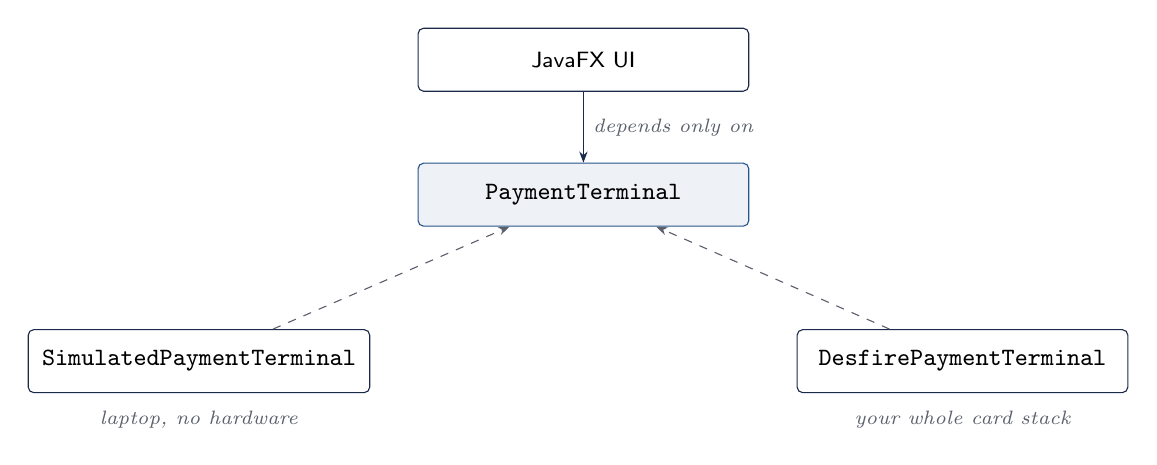
\begin{tikzpicture}[font=\footnotesize\sffamily,
   b/.style={draw=brewernavy, rounded corners=2pt, inner sep=5pt,
             minimum width=42mm, minimum height=8mm},
   i/.style={draw=brewerblue, fill=brewerblue!8, rounded corners=2pt,
             inner sep=5pt, minimum width=42mm, minimum height=8mm}]
  \node[b] (ui) {JavaFX UI};
  \node[i, below=9mm of ui] (if) {\code{PaymentTerminal}};
  \node[b, below left=13mm and 6mm of if] (sim) {\code{SimulatedPaymentTerminal}};
  \node[b, below right=13mm and 6mm of if] (real) {\code{DesfirePaymentTerminal}};
  \draw[-{Stealth[length=4pt]}, brewernavy] (ui) --
       node[right, font=\scriptsize\itshape, color=brewergrey] {depends only on} (if);
  \draw[-{Stealth[length=4pt]}, dashed, brewergrey] (sim) -- (if);
  \draw[-{Stealth[length=4pt]}, dashed, brewergrey] (real) -- (if);
  \node[font=\scriptsize\itshape, color=brewergrey, below=1mm of sim] {laptop, no hardware};
  \node[font=\scriptsize\itshape, color=brewergrey, below=1mm of real, align=center]
       {your whole card stack};
\end{tikzpicture}
\end{center}

The same seam idea as \code{SpiLink} and \code{ApduChannel}, now at the top of
the stack. It means the entire UI can be built and tested before a single card
exists, and the kiosk degrades gracefully: no reader attached, so use the
simulator, and the app still runs.

\section{The contract}

\begin{jcode}
package com.midnightbrewer.payment;

/**
 * The seam between the kiosk UI and whatever actually takes the money.
 *
 * The UI depends only on this type, so it neither knows nor cares whether
 * payment is a simulated wallet or a real DESFire being debited over SPI.
 *
 * Extends AutoCloseable so the RF field is always powered down, even on a
 * crash.
 */
public interface PaymentTerminal extends AutoCloseable {

    /**
     * Begin waiting for a card and charge it for drink.
     *
     * MUST return immediately -- all polling happens on a background thread.
     * Exactly one terminal callback (approved or declined) is delivered per
     * call, unless cancel() intervenes.
     */
    void startTransaction(Drink drink, PaymentListener listener);

    /** Abort the in-flight transaction. Safe to call when nothing is running. */
    void cancel();

    /** Human-readable state for the status pill, e.g. "RC522 READY". */
    String getStatusText();

    @Override
    void close();
}
\end{jcode}

\begin{jcode}
public interface PaymentListener {
    /** A card entered the field. Not yet authenticated. */
    void onCardDetected(String uid);
    /** Authenticated and balance read, before any debit. */
    void onBalanceRead(int balanceCents);
    /** Debit COMMITTED. The drink may now be dispensed. */
    void onApproved(PaymentReceipt receipt);
    /** Failed. The card was not charged, or the debit was rolled back. */
    void onDeclined(CardException cause);
}
\end{jcode}

\begin{concept}{Why callbacks, and why four of them}
\textbf{Why not a return value?} Because \code{startTransaction} returns
instantly and the result arrives seconds later. A blocking \code{boolean
pay(Drink)} would freeze the UI thread: the animation stops, touches queue up,
and the operating system offers to kill your app.

\textbf{Why four callbacks?} So the UI can narrate. ``Card detected\ldots'' then
``Balance \texteuro5.00, charging\ldots'' then approved. A payment terminal that
shows nothing for four seconds feels broken even when it is working perfectly.
\end{concept}

\section{The Adapter}
\index{Adapter pattern}

Now the interesting class: something that satisfies \code{PaymentTerminal} by
driving the stack you built in Parts~II--IV.

\begin{analogy}{The travel plug adapter}
Your laptop charger has one plug shape; the Italian wall has another. The adapter
does not generate electricity or modify the laptop --- it sits between two fixed
interfaces and translates.

Both sides were designed without knowledge of each other, and the adapter makes
them fit. Here the kiosk speaks \code{PaymentTerminal} and \code{CardException};
your stack speaks \code{Rc522Reader}, \code{DesfireCard} and
\code{SpiException}. \code{DesfirePaymentTerminal} translates --- including the
exceptions, so a \code{com.midnightbrewer.hardware} type never leaks into the UI.
\end{analogy}

\begin{jcode}
package com.midnightbrewer.payment;

public class DesfirePaymentTerminal implements PaymentTerminal {

    // How the card was personalised (Chapter 12 / Appendix A).
    private static final byte[] APP_AID       = { 0x03, 0x02, 0x01 };
    private static final byte   USER_KEY_NO   = 0x02;
    private static final byte   VALUE_FILE_NO = 0x01;

    private final Pi4jSpiLink link;
    private final Rc522Driver driver;
    private final Rc522Reader reader;

    // ONE background thread, created once. Transactions are strictly
    // sequential -- two overlapping card conversations would interleave
    // command counters and corrupt both.
    private final ExecutorService worker =
            Executors.newSingleThreadExecutor(r -> {
                Thread t = new Thread(r, "desfire-terminal");
                t.setDaemon(true);      // never blocks JVM shutdown
                return t;
            });

    /** Written by the UI thread, read by the worker. */
    private final AtomicBoolean cancelled = new AtomicBoolean(false);
    private volatile boolean scanning = false;

    /** Opens the reader. THROWS if there is no RC522 -- see createTerminal(). */
    public DesfirePaymentTerminal() throws SpiException {
        this.link = new Pi4jSpiLink();
        this.driver = new Rc522Driver(link);
        try {
            initReader();
            int version = driver.version();
            if (version != 0x91 && version != 0x92) {
                throw new SpiException("RC522 not responding");
            }
        } catch (SpiException e) {
            quietClose();               // do not leak SPI on a failed construction
            throw e;
        }
        this.reader = new Rc522Reader(driver);
    }

    @Override
    public void startTransaction(Drink drink, PaymentListener listener) {
        cancelled.set(false);
        worker.submit(() -> runTransaction(drink, listener));   // returns instantly
    }

    private void runTransaction(Drink drink, PaymentListener listener) {
        scanning = true;
        try {
            // Fresh reader state each tap: softReset + antennaOn power-cycles
            // the field so the card is IDLE again and activate() runs cleanly
            // even after a previous purchase.
            initReader();

            if (!waitForCard()) return;         // cancelled; the UI moved on

            ActivatedCard card = reader.activate();
            listener.onCardDetected(card.uidHex());

            DesfireCard desfire = new DesfireCard(
                    new IsoDepChannel(reader), RandomSource.secure());
            desfire.selectApplication(APP_AID);
            desfire.authenticateEv2First(USER_KEY_NO, userKey());

            int balance = desfire.getValue(VALUE_FILE_NO);
            listener.onBalanceRead(balance);

            int price = drink.getPriceCents();
            if (balance < price) {
                listener.onDeclined(new InsufficientFundsException(balance, price));
                return;
            }

            // Provisional until the commit is acknowledged; only THEN may we
            // hand out a receipt, and only then may the UI dispense.
            desfire.debit(VALUE_FILE_NO, price);
            desfire.commitTransaction();
            int after = desfire.getValue(VALUE_FILE_NO);

            listener.onApproved(
                new PaymentReceipt(card.uidHex(), drink, balance, after));

        } catch (SpiException e) {
            listener.onDeclined(translate(e));  // stack vocabulary -> UI vocabulary
        } catch (RuntimeException e) {
            listener.onDeclined(new CardCommunicationException(
                    "unexpected reader error: " + e.getMessage(), e));
        } finally {
            scanning = false;
        }
    }

    private boolean waitForCard() throws SpiException {
        while (!cancelled.get()) {
            if (reader.isCardPresent()) return true;
            sleep(30);
        }
        return false;
    }
}
\end{jcode}

\begin{concept}{\texttt{catch (RuntimeException)} is not paranoia}
A kiosk must never die on a bad tap. \code{SpiException} covers expected
failures; the \code{RuntimeException} catch covers the unexpected --- an array
index, a null, a Pi4J internal error.

Without it, one odd card kills the worker thread and the machine stops taking
payments until someone reboots it.

\textbf{At a process boundary, catch broadly and report. Inside your logic, catch
narrowly.}
\end{concept}

\section{Threading: the rule you must not break}

JavaFX has exactly one thread allowed to touch the UI. Your terminal calls back
from a \emph{different} thread. So every callback hops:

\begin{jcode}
private final class UiPaymentListener implements PaymentListener {

    @Override
    public void onCardDetected(String uid) {
        Platform.runLater(() ->
            paymentHintLabel.setText("Card detected -- authenticating..."));
    }

    @Override
    public void onApproved(PaymentReceipt receipt) {
        Platform.runLater(() -> { stopPulse(); startBrewing(receipt); });
    }
}
\end{jcode}

\begin{trap}{Off-thread UI access does not reliably throw}
Sometimes it works. Sometimes it corrupts rendering in ways that appear once an
hour, on the real panel only, and never under a debugger.

This is one of the nastiest bug classes in UI programming, and the fix is a
habit, not a diagnosis: \textbf{every callback that touches the scene graph is
wrapped in \code{Platform.runLater}.} No exceptions.

The same rule exists everywhere: Android has \code{runOnUiThread}, Swing has
\code{invokeLater}, Qt has queued connections. One thread owns the widgets.
\end{trap}

\section{Choosing the backend}

The whole design collapses into one method:

\begin{jcode}
private PaymentTerminal createTerminal() {
    if ("simulated".equalsIgnoreCase(System.getProperty("brewer.reader", ""))) {
        return new SimulatedPaymentTerminal();          // forced, for UI work
    }
    try {
        PaymentTerminal real = new DesfirePaymentTerminal();
        System.out.println("[UI] RC522 ready -- real card payment enabled");
        return real;
    } catch (Exception e) {
        System.out.println("[UI] no RC522 (" + e.getMessage()
                + ") -- using the simulator");
        return new SimulatedPaymentTerminal();
    }
}
\end{jcode}

\textbf{Detection by attempting to open.} On a laptop, constructing
\code{Pi4jSpiLink} throws and you fall back. The same build runs everywhere: no
flags, no config file, no \code{\#ifdef}. This is precisely why the constructor
\emph{must} throw rather than returning a half-built object.

And because everything above depends on the interface, the UI needs
\textbf{zero} changes to switch backends. The bench ``simulate tap'' button even
hides itself:

\begin{jcode}
devTapButton.setVisible(terminal instanceof SimulatedPaymentTerminal);
\end{jcode}

\section{Verify}

\textbf{On a laptop} (no hardware): \code{mvn javafx:run -Dbrewer.windowed=true}.
The simulator's tap button drives the whole flow.

\textbf{On the Pi}, run a headless smoke test first --- it exercises the exact
path a tap takes, minus the screen:

\begin{jcode}
public final class TerminalCheck {
    public static void main(String[] args) throws Exception {
        Drink testDrink = new Drink("test", "Test Shot", 10);   // 10 cents
        try (DesfirePaymentTerminal terminal = new DesfirePaymentTerminal()) {
            CountDownLatch done = new CountDownLatch(1);
            terminal.startTransaction(testDrink, new PaymentListener() {
                public void onCardDetected(String uid)   { print("card: " + uid); }
                public void onBalanceRead(int cents)     { print("balance: " + cents); }
                public void onApproved(PaymentReceipt r) { print("APPROVED"); done.countDown(); }
                public void onDeclined(CardException e)  { print("DECLINED"); done.countDown(); }
            });
            System.out.println("Tap a card...");
            done.await();
        }
    }
}
\end{jcode}

\code{CountDownLatch} is how \code{main} waits for a background thread: start at
one, block on \code{await()}, and the callback counts down to zero to release it.

\begin{verifybox}
\begin{trace}
  card: 04 76 18 62 7B 20 90
  balance: $5.00
  APPROVED: charged $0.10  ($5.00 -> $4.90)
\end{trace}
\end{verifybox}

\section{Traps}

\begin{traptable}
UI freezes on tap & Card work on the FX thread. It must be on the worker. \\
Random rendering corruption & A callback touching nodes without \code{Platform.runLater}. \\
Second tap always fails & Reader not re-initialised per transaction. \\
Kiosk dies on an odd card & Missing the broad \code{RuntimeException} catch. \\
Simulator used on the Pi & Constructor threw --- read the printed message, it names the cause. \\
Drink dispensed but card not charged & Dispensing on \code{debit} instead of after \code{commitTransaction}. \\
\end{traptable}

\section{Commit}

\begin{shell}
git add -A
git commit -m "kiosk: PaymentTerminal seam + DesfirePaymentTerminal adapter"
\end{shell}

\chapter{The Android top-up app}
\label{ch:android}

\chapterbrief
  {Put credit \emph{onto} the card from a phone. Build it yourself, in Dart, from the design you already understand.}
  {Porting a design across languages --- and discovering how much of your stack was incidental.}
  {A phone that adds credit, and cross-language proof your crypto is right.}

\section{Why this chapter is different}

You have built the whole reader stack once. The point of this chapter is not to
learn NFC again. It is to discover something valuable:

\begin{center}\bfseries\itshape
Six of your ten chapters do not exist on Android.
\end{center}

The phone has an NFC controller with a driver already written. Android's
\code{IsoDep} class hands you \code{transceive(byte[]) -> byte[]} directly. That
single method is everything you built in Chapters~\ref{ch:spi}--\ref{ch:apdu}.

\begin{center}\small
\begin{tabular}{@{}L{0.42\linewidth}L{0.48\linewidth}@{}}
\toprule
\thead{Your Pi stack} & \thead{Android} \\
\midrule
Ch.~\ref{ch:spi} \code{SpiLink}         & \emph{gone} --- the OS owns the radio \\
Ch.~\ref{ch:driver} \code{Rc522Driver}  & \emph{gone} \\
Ch.~\ref{ch:reader} \code{Rc522Reader}  & \emph{gone} \\
Ch.~\ref{ch:blocks} \code{ProtocolBlock}& \emph{gone} --- the OS frames I-blocks \\
Ch.~\ref{ch:activation} activation      & \emph{gone} --- you are handed an activated tag \\
Ch.~\ref{ch:apdu} \code{IsoDepChannel}  & \textbf{\code{IsoDep.transceive()}} \\
\midrule
\textbf{Ch.~\ref{ch:cmac}--\ref{ch:secmsg} crypto} & \textbf{you port all of it, unchanged} \\
\bottomrule
\end{tabular}
\end{center}

\begin{concept}{The transport was replaceable; the protocol was the work}
Look at the shape of your \code{ApduChannel} interface from
Chapter~\ref{ch:apdu} and Android's \code{IsoDep.transceive}. They are the same.

That is not luck --- it is what happens when you draw a seam at the right place.
Everything above \code{ApduChannel} ports across a language, an operating system,
and a completely different radio, without changing.

If you want one test of whether an abstraction was well chosen, this is it:
\emph{how much survives when the thing underneath is replaced entirely?}
\end{concept}

\begin{analogy}{Posting the letter}
You have been writing a letter and hand-delivering it. Now you are posting it.
The envelope, the courier, the van --- all different. The letter is identical.
\end{analogy}

\section{Setup}

\begin{shell}
flutter create --org com.midnightbrewer --platforms android topup_app
cd topup_app
\end{shell}

\begin{xcode}
dependencies:
  flutter:
    sdk: flutter
  # Android IsoDep (ISO 14443-4) transceive.
  # 4.x has a different API from 3.x -- pin the major version.
  nfc_manager: ^4.2.1
  # AES-ECB/CBC and AES-CMAC.
  pointycastle: ^4.0.0
\end{xcode}

And in \code{android/app/src/main/AndroidManifest.xml}:

\begin{xcode}
<uses-permission android:name="android.permission.NFC" />
<uses-feature android:name="android.hardware.nfc" android:required="true" />
\end{xcode}

\section{Dart for a Java programmer}

The languages are close cousins. Four differences matter here.

\begin{description}[leftmargin=0pt, style=nextline]
  \item[\code{Uint8List}, not \code{byte[]}.] From \code{dart:typed\_data}.
        Crucially its elements are \textbf{unsigned 0--255}: Dart has no
        signed-byte trap, and all those \code{\& 0xFF} masks simply vanish.
  \item[\code{int} is 64-bit.] So \code{1 << 40} works fine, but when writing a
        32-bit value you must mask deliberately: \code{(v >> 24) \& 0xFF}.
  \item[Async is explicit.] NFC calls are \code{Future}s. A function that awaits
        must be \code{async}, and its callers must \code{await} it --- the
        colouring propagates upward, much as \code{throws SpiException} did in
        Java. Same discipline, different keyword.
  \item[No checked exceptions.] Dart has \code{throw}/\code{catch} but the
        compiler forces nothing. You lose the nagging, so you must be more
        deliberate about error paths.
\end{description}

\section{Build it}

\subsection{The transport --- one class replaces six chapters}

\begin{dcode}
import 'dart:typed_data';
import 'package:nfc_manager/nfc_manager.dart';

/// Sends one APDU to an activated card and returns the reply.
///
/// This is the ENTIRE transport layer -- the Android NFC stack has already
/// done activation, anticollision, RATS and ISO-DEP framing for us.
/// Compare Chapters 2-7 of the Pi build. Same seam, no work.
class IsoDepTransceiver {
  IsoDepTransceiver(this._isoDep);

  final IsoDep _isoDep;

  Future<Uint8List> transceive(Uint8List apdu) async {
    // TODO: return await _isoDep.transceive(data: apdu);
    //   Wrap failures in your own exception type so the UI never sees a
    //   platform exception -- the same translate() discipline as Chapter 12.
    throw UnimplementedError();
  }
}
\end{dcode}

\subsection{The crypto --- port it directly}

Your Java from Chapters~\ref{ch:cmac}--\ref{ch:secmsg} translates almost line for
line. \code{pointycastle} supplies AES \emph{and} CMAC, so you do not even
reimplement RFC 4493 --- but you must verify it produces the same bytes.

\begin{dcode}
import 'dart:typed_data';
import 'package:pointycastle/export.dart';

const int kAesBlockSize = 16;

Uint8List aesEcbEncryptBlock(Uint8List key, Uint8List block) {
  final engine = AESEngine()..init(true, KeyParameter(key));
  final out = Uint8List(kAesBlockSize);
  engine.processBlock(block, 0, out, 0);
  return out;
}

Uint8List aesCbcEncrypt(Uint8List key, Uint8List iv, Uint8List data) {
  // TODO: CBCBlockCipher(AESEngine())
  //         ..init(true, ParametersWithIV(KeyParameter(key), iv));
  //       process block by block; NO padding (DESFire pads itself).
  throw UnimplementedError();
}

Uint8List aesCmac(Uint8List key, Uint8List message) {
  final mac = CMac(AESEngine(), 128)..init(KeyParameter(key));
  return mac.process(message);
}

/// DESFire keeps the ODD-indexed bytes: mac[1], mac[3], ... mac[15].
Uint8List truncateMac(Uint8List mac) {
  // TODO: 8 bytes, out[i] = mac[i * 2 + 1];
  throw UnimplementedError();
}

/// The 32-byte derivation vector, exactly as in Chapter 9.
Uint8List deriveSessionKey(
    Uint8List key, Uint8List rndA, Uint8List rndB, int label) {
  // TODO: sv[0] = label (0xA5 enc / 0x5A mac); sv[1] = the other;
  //       sv[2..5] = 00 01 00 80;
  //       sv[6..7] = rndA[0..1];
  //       sv[8..13] = rndA[2..7] ^ rndB[0..5];
  //       sv[14..23] = rndB[6..15];
  //       sv[24..31] = rndA[8..15];
  //       return aesCmac(key, sv);
  throw UnimplementedError();
}

/// ISO 7816-4: append 0x80 then zeros. ALWAYS adds at least one byte.
Uint8List padIso7816(Uint8List data) {
  final paddedLength = (data.length | 0x0F) + 1;
  final out = Uint8List(paddedLength);
  out.setRange(0, data.length, data);
  out[data.length] = 0x80;
  return out;
}
\end{dcode}

\begin{verifybox}
\textbf{Verify with the same vectors.} This is the elegant part: the vectors in
Appendix~\ref{app:vectors} are language-agnostic. Your Dart must produce
byte-for-byte what your Java produced.

\begin{dcode}
void main() {
  test('derives the Chapter 9 session keys', () {
    final key  = fromHex('00112233445566778899aabbccddeeff');
    final rndA = fromHex('a0a1a2a3a4a5a6a7a8a9aaabacadaeaf');
    final rndB = fromHex('b0b1b2b3b4b5b6b7b8b9babbbcbdbebf');

    expect(toHex(deriveSessionKey(key, rndA, rndB, 0xA5)),
           'd46c03528ecd3b1f1148e708d3e9729d');
    expect(toHex(deriveSessionKey(key, rndA, rndB, 0x5A)),
           '116d156cc502da820eb57915f189ec74');
  });

  test('truncates a CMAC to the odd bytes', () {
    expect(toHex(truncateMac(fromHex('00112233445566778899aabbccddeeff'))),
           '1133557799bbddff');
  });
}
\end{dcode}

\begin{shell}
flutter test           # no phone, no card -- same discipline as the Pi build
\end{shell}

If your Dart disagrees with your Java on any vector, \textbf{one of them is
wrong}, and you now know before either touches a card. Two independent
implementations converging on the same bytes is much stronger evidence than
either alone.
\end{verifybox}

\subsection{Credit --- the mirror image of debit}

\begin{dcode}
/// Credit (0x0C) in CommMode.Full -- the mirror image of Debit.
///
/// Identical wire format; only the command byte differs. Like debit it only
/// STAGES the change: nothing moves until commitTransaction().
Future<void> credit(int fileNo, int amountCents) async {
  // TODO: same shape as Chapter 11's debit:
  //   header     = [fileNo]
  //   ciphertext = session.encryptCommandData(encodeValue(amountCents))
  //   macInput   = header + ciphertext
  //   mac        = session.commandMac(0x0C, macInput)
  //   send, check status, incrementCounter, verify response MAC over empty
  throw UnimplementedError();
}
\end{dcode}

And the top-up sequence, which reads the balance back:

\begin{dcode}
Future<int> topUp(int fileNo, int amountCents) async {
  final before = await getValue(fileNo);
  await credit(fileNo, amountCents);
  await commitTransaction();
  final after = await getValue(fileNo);      // trust nothing; re-read

  if (after != before + amountCents) {
    throw StateError('balance did not move as expected');
  }
  return after;
}
\end{dcode}

Reading the balance back after the commit is not paranoia --- it is the only way
to \emph{know}. If the phone loses the field between \code{credit} and
\code{commitTransaction}, the card discards the delta and the balance is
unchanged. Same safety property as Chapter~\ref{ch:secmsg}, now protecting your
customer's money rather than yours.

\section{Provisioning: turning a blank card into a wallet}

A factory-fresh DESFire has no application, no value file, and a DES master key.
To make one work with your kiosk:

\begin{enumerate}
  \item authenticate at PICC level with the master key (16 $\times$ \hex{0x00} factory default);
  \item \code{CreateApplication} (\hex{0xCA}) --- AID \hex{0x010203}, 3 keys, AES;
  \item select the application, authenticate with its master key (initially 16 $\times$ \hex{0x00});
  \item \code{ChangeKey} (\hex{0xC4}) --- set app master key (\hex{0x11}\ldots) and user key (\hex{0x22}\ldots);
  \item re-authenticate with the new app master key;
  \item \code{CreateValueFile} (\hex{0xCC}) --- file \hex{0x01}, CommMode.Full,
        access via key 2, limits 0\ldots100000, initial value 0.
\end{enumerate}

Wire format for \code{CreateValueFile}, 17 bytes:

\begin{trace}
[0]      fileNo
[1]      commSettings          0x03 = Full
[2..3]   accessRights          little-endian; nibbles: read|write|rw|changeRights
[4..7]   lowerLimit            signed LE
[8..11]  upperLimit            signed LE
[12..15] initialValue          signed LE
[16]     limitedCreditEnabled  0x00 / 0x01
\end{trace}

The access-rights word packs four 4-bit key numbers: \emph{read} (GetValue),
\emph{write} (Debit), \emph{readWrite} (Credit too), and
\emph{changeAccessRights}. Using key 2 for all four gives \hex{0x2222}. Nibble
\hex{0xE} means free access; \hex{0xF} means never.

\begin{trap}{\texttt{ChangeKey} is irreversible}
Set a key to a value you do not record and that card is scrap --- permanently, by
design. There is no recovery path; that \emph{is} the security property.

Before you run provisioning:
\begin{itemize}
  \item use \textbf{dedicated test cards} you bought for this project;
  \item never change the PICC master key from its factory default (this project
        deliberately does not, so any other tool can re-personalise the card);
  \item never point this at a card you did not buy for this --- the DESFire in
        your wallet may be your office badge or transit pass, and it will not
        survive.
\end{itemize}

And \textbf{never auto-provision on tap}. Require an explicit ``Set up this
card'' button press. A member of the public tapping your app must never have
their existing card silently rewritten.
\end{trap}

\section{The security reality of hardcoded keys}
\label{sec:realkeys}

Your app will contain, in plaintext, the AES keys for every card in the fleet.
Anyone who pulls the APK off a phone can extract them and mint unlimited balance
on every card you have issued.

\textbf{For a bench project with test cards this is fine.} Say so out loud, in a
comment, so nobody mistakes it for a design:

\begin{dcode}
/// BENCH KEYS. These are compiled into the APK in plaintext. Anyone who pulls
/// the APK can read them and mint unlimited balance on every card, because the
/// same key is on every card. Acceptable for a bench rig with test cards.
/// NOT acceptable for anything representing real money.
\end{dcode}

\begin{concept}{What a real deployment does instead}
Worth understanding even if you never build it.

\textbf{1. Key diversification.} Each card gets a \emph{different} key, derived
from the card's UID and a master key (typically via CMAC). Compromise one card
and you learn one card's key --- not the fleet's.

\textbf{2. A backend HSM or SAM.} The master key never leaves tamper-resistant
hardware. The phone becomes a dumb pipe: it relays APDUs between the card and the
server, and the \emph{server} performs the cryptography.

\textbf{3. Server-side transaction logs}, so the balance on the card is a cache
rather than the source of truth, and double-spends are detectable after the fact.

The gap between ``works'' and ``safe to deploy'' is mostly key management, and it
is why payment systems have HSMs. Knowing exactly where your bench rig sits on
that spectrum is the professional part.
\end{concept}

\section{Build order}

Do it in this order:

\begin{enumerate}
  \item \code{flutter create} plus dependencies; blank app runs on your phone.
  \item \textbf{Crypto module and tests.} No NFC yet. All vectors green.
  \item \code{IsoDepTransceiver} and a ``read the card's version'' screen. Prove
        \hex{90 60 00 00 00} returns \hex{...91AF}.
  \item \code{authenticateEv2First}, on a card the kiosk already works with.
  \item \code{getValue} --- display the balance. Read-only, so mistakes are harmless.
  \item \code{credit} $+$ \code{commit} $+$ read-back. Now money moves.
  \item Provisioning screen, last, behind an explicit button.
  \item UI polish --- the NFC pulse animation, preset amounts, result screen.
\end{enumerate}

Steps 2 and 5 are the natural stopping points if you are filming: ``the crypto
agrees across two languages'' and ``the phone reads the balance the Pi wrote''.

\section{Traps}

\begin{traptable}
\code{nfc\_manager} API does not match tutorials & 3.x and 4.x differ. Pin 4.x and use its docs. \\
Works on one phone, not another & NFC antenna placement varies enormously. Try the upper third of the back. \\
Tag lost mid-transaction & Phone moved. This is \emph{normal} --- it is why commit exists. Handle it. \\
Dart and Java disagree on a MAC & Almost always the counter or TI, not the AES. Print both inputs. \\
\hex{91 AE} after provisioning & You changed a key and re-authenticated with the old one. \\
Card bricked & You changed a key you did not record. There is no recovery. This is why you buy spares. \\
\end{traptable}

\section{Commit}

\begin{shell}
git add -A
git commit -m "topup: Flutter app -- crypto ported, credit + commit, provisioning"
\end{shell}

\chapter{Deploying to the Pi}
\label{ch:deploy}

\chapterbrief
  {The machine boots into the kiosk: fullscreen, correctly rotated, GPU-accelerated, no keyboard attached.}
  {Operational discipline --- the difference between a demo and a machine.}
  {Something you can hang on a wall and walk away from.}

\section{Rotating the display}

A 7-inch panel mounted vertically needs the \emph{compositor} rotated, not the
app. Raspberry Pi OS (Bookworm and later) uses \textbf{labwc} on Wayland.

\code{\textasciitilde/.config/labwc/autostart}:

\begin{shell}
# 1024x600 panel mounted rotated -> the app sees a 600x1024 portrait screen.
wlr-randr --output HDMI-A-1 --transform 90 &
\end{shell}

Check your output name with \code{wlr-randr}; it may be \code{HDMI-A-2}.

\textbf{Touch must be rotated too}, and this is the step everyone forgets. An
unrotated touchscreen on a rotated display gives inverted axes: you press the
top-left tile and the bottom-right one activates. Maddening, and it looks like a
UI bug.

In \code{\textasciitilde/.config/labwc/rc.xml}, inside \code{<libinput>}:

\begin{xcode}
<device category="touch">
  <transformationMatrix>0 -1 1 1 0 0</transformationMatrix>
</device>
\end{xcode}

That matrix is a 90\textdegree{} rotation. For 270\textdegree{} use
\code{0 1 0 -1 0 1}. If touch ends up mirrored rather than rotated, you have the
wrong one.

\begin{concept}{Why the app does not rotate itself}
If JavaFX rendered rotated, every animation would run through a transform, the
compositor would still composite unrotated, and touch would \emph{still} be
wrong.

Rotating at the compositor means everything below it --- including input --- is
consistently transformed, and the app simply sees a portrait screen. Apply a
transformation at the lowest layer that owns all the affected data.
\end{concept}

\section{GPU acceleration: the one flag that matters}

JavaFX on a Pi will silently fall back to software rendering, and the difference
is night and day: a fade that takes 16\,ms on the GPU takes 400\,ms on the CPU,
and your kiosk feels broken.

The cause is specific. The VideoCore VI driver reports \textbf{OpenGL 2.1}, and
JavaFX's Prism pipeline checks for a higher version and refuses. The GPU is
perfectly capable; the version check is wrong.

\begin{shell}
java -Dprism.forceGPU=true \
     -Dprism.verbose=true \
     -cp "target/classes:target/dependency/*" com.midnightbrewer.ui.MainApp
\end{shell}

\code{-Dprism.verbose=true} prints the chosen pipeline at startup. You want to
see \code{es2} (hardware). If it says \code{sw}, you are on the CPU.

Also worth setting in \code{/boot/firmware/config.txt}:

\begin{shell}
dtoverlay=vc4-kms-v3d
gpu_mem=128
\end{shell}

\subsection{Other things that mattered on a Zero 2 W}

\begin{itemize}
  \item \textbf{Cache the pulse rings.} \code{ring.setCache(true);
        ring.setCacheHint(CacheHint.SPEED);} Without it, JavaFX re-rasterises the
        vector circle every frame while it scales. With it, you are scaling a
        bitmap, which is nearly free.
  \item \textbf{Hide the cursor} (\code{scene.setCursor(Cursor.NONE)}). Xwayland
        parks a pointer mid-screen; it sits on a tile and leaves it stuck in
        \code{:hover}, which reads as a pre-selected drink.
  \item \textbf{Scope hover styling} to a \code{.desktop} CSS class you enable
        only in windowed development mode. A touchscreen has no hover state to
        represent.
\end{itemize}

\section{Autostart with systemd}

\code{/etc/systemd/system/midnight-brewer.service}:

\begin{shell}
[Unit]
Description=The Midnight Brewer kiosk
After=graphical.target

[Service]
Type=simple
User=martin
Environment=WAYLAND_DISPLAY=wayland-0
Environment=XDG_RUNTIME_DIR=/run/user/1000
WorkingDirectory=/home/martin/midnight-brewer
ExecStart=/usr/bin/java -Dprism.forceGPU=true \
    -cp "target/classes:target/dependency/*" com.midnightbrewer.ui.MainApp
Restart=always
RestartSec=5

[Install]
WantedBy=graphical.target
\end{shell}

\begin{shell}
sudo systemctl daemon-reload
sudo systemctl enable --now midnight-brewer
journalctl -u midnight-brewer -f      # watch it
\end{shell}

\begin{concept}{\texttt{Restart=always} is the important line}
A kiosk that dies at three in the morning and stays dead is worse than one that
restarts in five seconds.

Combined with the broad \code{catch (RuntimeException)} from
Chapter~\ref{ch:kiosk}, you have two layers of resilience: bad taps do not kill
the worker thread, and a fatal crash does not kill the machine.

Design for the failure you cannot foresee by making recovery automatic.
\end{concept}

Remember the group membership, or Pi4J cannot open the device:

\begin{shell}
sudo usermod -aG spi,gpio martin      # log out and back in
\end{shell}

\section{The deploy loop}

Compiling on a Zero 2 W is slow enough to break your concentration. Two options.

\textbf{Rsync the source, build on the Pi} (simple, about 40 seconds):

\begin{shell}
rsync -av --exclude target/ ./ martin@raspberrypi.local:~/midnight-brewer/
ssh martin@raspberrypi.local 'cd ~/midnight-brewer && mvn -q -DskipTests compile'
\end{shell}

\textbf{Or build locally and ship the classes} (about 5 seconds). Java bytecode
is architecture-independent, so a laptop build runs unchanged on ARM:

\begin{shell}
mvn -q -DskipTests compile
rsync -av target/classes/ martin@raspberrypi.local:~/midnight-brewer/target/classes/
\end{shell}

Do the dependency copy \emph{once}:

\begin{shell}
ssh martin@raspberrypi.local \
  'cd ~/midnight-brewer && mvn dependency:copy-dependencies -DincludeScope=runtime'
\end{shell}

\begin{trap}{Stale classes}
If you change a file and the old \code{.class} survives, you will debug behaviour
that no longer exists in your source.

When something makes no sense \emph{at all} --- when the code in front of you
cannot possibly produce the output you are seeing --- run \code{mvn clean
compile} before anything else.
\end{trap}

\section{Field hygiene}

Three habits that keep a kiosk healthy.

\begin{description}[leftmargin=0pt, style=nextline]
  \item[Power-cycle the RF field per transaction.] \code{softReset()} $+$
        \code{antennaOn()} at the start of each tap puts any lingering card back
        to IDLE. Without it, a card left on the antenna after one purchase is in
        the wrong state for the next.
  \item[Always close the link.] try-with-resources on \code{Pi4jSpiLink}, and
        \code{close()} in the JavaFX \code{stop()} hook. An RF field left
        energised overnight cooks the module.
  \item[Never log key material.] It is tempting during debugging to print session
        keys. If that line survives into production, your logs are now a key
        store. Print the \emph{TI} and the \emph{counter} instead --- they tell
        you everything you need for protocol debugging and nothing an attacker
        wants.
\end{description}

\section{The finished machine}

\begin{center}
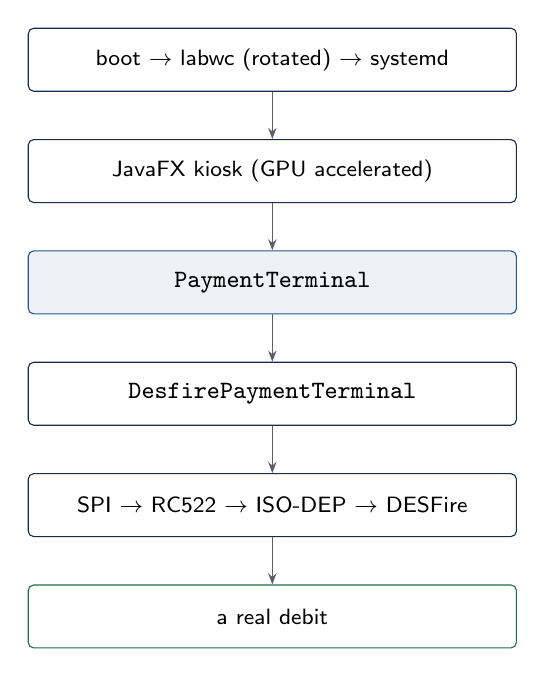
\begin{tikzpicture}[font=\footnotesize\sffamily, node distance=6mm,
   b/.style={draw=brewernavy, rounded corners=2pt, minimum width=62mm,
             minimum height=8mm, inner sep=3pt}]
  \node[b] (boot) {boot $\rightarrow$ labwc (rotated) $\rightarrow$ systemd};
  \node[b, below=of boot] (fx) {JavaFX kiosk (GPU accelerated)};
  \node[b, below=of fx, draw=brewerblue, fill=brewerblue!8] (pt) {\code{PaymentTerminal}};
  \node[b, below=of pt] (dpt) {\code{DesfirePaymentTerminal}};
  \node[b, below=of dpt] (stack) {SPI $\rightarrow$ RC522 $\rightarrow$ ISO-DEP $\rightarrow$ DESFire};
  \node[b, below=of stack, draw=brewergreen] (debit) {a real debit};
  \foreach \a/\bb in {boot/fx, fx/pt, pt/dpt, dpt/stack, stack/debit}{
    \draw[-{Stealth[length=4pt]}, brewergrey] (\a) -- (\bb);}
\end{tikzpicture}
\end{center}

\section{Commit}

\begin{shell}
git add -A
git commit -m "deploy: rotation, GPU flag, systemd unit, deploy scripts"
\end{shell}


% ============================================================
\appendix
\part{Appendices}
\chapter{Test vectors}
\label{app:vectors}

Everything you need to verify the cryptography offline, in one place. All values
are hexadecimal, lowercase, unspaced.

\begin{concept}{Why these are trustworthy}
They were generated with Python's \code{cryptography} library, deliberately
\emph{not} with the Java you are writing. Agreement therefore means your
implementation is \textbf{correct}, not merely self-consistent.

Regenerate or extend them with \code{tools/m7d\_vectors.py} in the companion
repository.
\end{concept}

\section{AES-CMAC --- RFC 4493 (Chapter~\ref{ch:cmac})}

\textbf{Key} $K = $ \hex{2b7e151628aed2a6abf7158809cf4f3c}

Subkeys:
\begin{trace}
K1 = fbeed618357133667c85e08f7236a8de
K2 = f7ddac306ae266ccf90bc11ee46d513b
\end{trace}

\begin{center}\small
\begin{tabular}{@{}cL{0.40\linewidth}L{0.40\linewidth}@{}}
\toprule
\thead{\#} & \thead{Message} & \thead{CMAC} \\
\midrule
1 & \emph{(empty)} & \hex{bb1d6929e95937287fa37d129b756746} \\
2 & \hex{6bc1bee22e409f96e93d7e117393172a} & \hex{070a16b46b4d4144f79bdd9dd04a287c} \\
3 & \hex{6bc1bee22e409f96e93d7e117393172a}\newline
    \hex{ae2d8a571e03ac9c9eb76fac45af8e51}\newline
    \hex{30c81c46a35ce411} & \hex{dfa66747de9ae63030ca32611497c827} \\
4 & message 3 $+$ \hex{e5fbc1191a0a52ef}\newline
    \hex{f69f2445df4f9b17ad2b417be66c3710} & \hex{51f0bebf7e3b9d92fc49741779363cfe} \\
\bottomrule
\end{tabular}
\end{center}

The four cases cover every branch: empty (pad, $K_2$), one full block ($K_1$),
partial last block (pad, $K_2$), and multiple full blocks ($K_1$).

\section{The reference session (Chapters~\ref{ch:sesskeys}--\ref{ch:secmsg})}

Every vector below derives from these three inputs. They are chained
deliberately: the same session runs through key derivation, the authentication
replay, and secure messaging, so a failure anywhere points at one specific step.

\begin{trace}
authKey = 00112233445566778899aabbccddeeff
rndA    = a0a1a2a3a4a5a6a7a8a9aaabacadaeaf     (pin this in tests)
rndB    = b0b1b2b3b4b5b6b7b8b9babbbcbdbebf
\end{trace}

\subsection{Session keys}

\begin{trace}
Kenc = d46c03528ecd3b1f1148e708d3e9729d      (label 0xA5)
Kmac = 116d156cc502da820eb57915f189ec74      (label 0x5A)
\end{trace}

\subsection{Byte rotation}

\begin{trace}
rotateLeft(b0b1b2b3b4b5b6b7b8b9babbbcbdbebf)
         = b1b2b3b4b5b6b7b8b9babbbcbdbebfb0
\end{trace}

\section{The authentication replay (Chapter~\ref{ch:auth})}

A complete \code{AuthenticateEV2First} exchange with \code{rndA} pinned. All AES
uses an \textbf{all-zero IV}.

\begin{center}\small
\begin{tabular}{@{}L{0.36\linewidth}L{0.54\linewidth}@{}}
\toprule
\thead{Direction} & \thead{Bytes} \\
\midrule
card $\rightarrow$ you, step 1 \newline $E(K, RndB)$ &
  \hex{eab6822fe368d5bc9895fb2558b38dde} \\
you $\rightarrow$ card, step 2 \newline $E(K, RndA \| RndB')$ &
  \hex{cf086a82c0b745a749daabb28a7a8db3}\newline
  \hex{32272f9e5fdc37a4746064f25b7c2ca7} \\
card $\rightarrow$ you, step 2 \newline $E(K, TI \| RndA' \| caps)$ &
  \hex{4e08e447d74810052caa1c5b6c60343f}\newline
  \hex{51f6e901ad171e677b100d3a34c925e4} \\
$\rightarrow$ extracted TI & \hex{11223344} \\
\bottomrule
\end{tabular}
\end{center}

\begin{trap}{Fake replies must carry their status word}
Your card code strips the last two bytes off every response, so a fake that
omits them chops real ciphertext.

\begin{trace}
step-1 reply = eab6822fe368d5bc9895fb2558b38dde + 91af
step-2 reply = 4e08e447d74810052caa1c5b6c60343f
               51f6e901ad171e677b100d3a34c925e4 + 9100
select reply = 9100
\end{trace}
\end{trap}

\textbf{Cross-check.} Decrypting \hex{eab6822f...} with \code{authKey} and a zero
IV must yield exactly \hex{b0b1b2b3b4b5b6b7b8b9babbbcbdbebf}. If it does, your
authentication vectors and your session-key vectors are consistent with each
other.

\section{Secure messaging (Chapter~\ref{ch:secmsg})}

Session as above, with \textbf{TI $=$ \hex{11223344}}.

\subsection{The MAC layer}

\begin{trace}
truncateMac(00112233445566778899aabbccddeeff) = 1133557799bbddff
\end{trace}
(literally the odd-indexed bytes --- verifiable by eye)

\begin{center}\small
\begin{tabular}{@{}L{0.30\linewidth}cL{0.26\linewidth}L{0.26\linewidth}@{}}
\toprule
\thead{Call} & \thead{ctr} & \thead{MAC input} & \thead{Result} \\
\midrule
\code{commandMac(0x6C, \{01\})} & 0 & \hex{6c00001122334401} & \hex{4d131ee17b482b16} \\
\code{responseMac(\{\})}        & 1 & \hex{00010011223344}   & \hex{6b082e8062d1a89d} \\
\bottomrule
\end{tabular}
\end{center}

\subsection{The crypto layer}

\begin{center}\small
\begin{tabular}{@{}L{0.38\linewidth}cL{0.44\linewidth}@{}}
\toprule
\thead{Call} & \thead{ctr} & \thead{Result} \\
\midrule
\code{commandIv()}  & 0 & \hex{dd42134cd6970980d22066cb00ab1b16} \\
\code{responseIv()} & 1 & \hex{cb73ae774aafd81868062906135969b9} \\
\code{padIso7816(96000000)} & --- & \hex{96000000800000000000000000000000} \\
\code{encryptCommandData(150)} & 0 & \hex{a2eb8f000bf3ddfe6e18e8859b284591} \\
\bottomrule
\end{tabular}
\end{center}

\hex{96 00 00 00} is 150 little-endian, a \texteuro1.50 amount.

\subsection{GetValue (balance 1000 cents)}

\begin{center}\small
\begin{tabular}{@{}L{0.34\linewidth}cL{0.48\linewidth}@{}}
\toprule
\thead{Item} & \thead{ctr} & \thead{Bytes} \\
\midrule
card's encrypted payload & 1 & \hex{7950692fc2f01e72b3cee290f7122b5c} \\
card's response MAC      & 1 & \hex{a44a7f2359b2f512} \\
decrypts to              &   & \hex{e8030000} $+$ \hex{80} padding $\rightarrow$ \textbf{1000} \\
\bottomrule
\end{tabular}
\end{center}

Full fake reply:
\hex{7950692fc2f01e72b3cee290f7122b5c} $+$ \hex{a44a7f2359b2f512} $+$ \hex{9100}

\subsection{Debit 150 cents, then Commit}

\begin{center}\small
\begin{tabular}{@{}L{0.34\linewidth}cL{0.48\linewidth}@{}}
\toprule
\thead{Item} & \thead{ctr} & \thead{Bytes} \\
\midrule
debit ciphertext           & 0 & \hex{a2eb8f000bf3ddfe6e18e8859b284591} \\
debit command MAC input    & 0 & \hex{dc00001122334401a2eb8f000b}\newline\hex{f3ddfe6e18e8859b284591} \\
debit command MAC          & 0 & \hex{27e5ea2cb8acad7d} \\
\textbf{debit APDU data}   & 0 & \hex{01a2eb8f000bf3ddfe6e18e885}\newline\hex{9b28459127e5ea2cb8acad7d} \\
debit response MAC         & 1 & \hex{6b082e8062d1a89d} \\
commit command MAC input   & 1 & \hex{c7010011223344} \\
commit command MAC         & 1 & \hex{4dc9859e1a783ee0} \\
commit response MAC        & 2 & \hex{febea1fcb55208ba} \\
\bottomrule
\end{tabular}
\end{center}

Watch the counter walk $0 \rightarrow 1 \rightarrow 2$. That progression
\emph{is} the increment-ordering rule made visible.

\section{Card personalisation}

The values the kiosk and the top-up app must agree on. Change them anywhere and
you must change them everywhere.

\begin{center}\small
\begin{tabular}{@{}L{0.30\linewidth}L{0.28\linewidth}L{0.32\linewidth}@{}}
\toprule
\thead{Setting} & \thead{Value} & \thead{Notes} \\
\midrule
Application ID       & \hex{0x010203}   & on the wire \hex{03 02 01} (\textbf{LSB-first}) \\
App master key no.   & 0 & \\
App \textbf{user} key no. & \textbf{2} & everyday operations \\
Value file no.       & \hex{0x01} & \\
Comm mode            & Full (\hex{0x03}) & encrypted $+$ MAC'd \\
Access rights        & key 2 for all four roles & word \hex{0x2222} \\
Lower limit          & 0 cents & \\
Upper limit          & 100000 cents & \texteuro1000 \\
PICC master key      & 16 $\times$ \hex{0x00} & factory default, never changed \\
App master key       & 16 $\times$ \hex{0x11} & bench key \\
App user key         & 16 $\times$ \hex{0x22} & bench key \\
\bottomrule
\end{tabular}
\end{center}

\begin{trap}{These are bench keys}
Identical on every card, hardcoded in the app, and published in this book. They
protect nothing. See Section~\ref{sec:realkeys} for what a real deployment does.
\end{trap}

\section{DESFire command reference}

\begin{center}\small
\begin{tabular}{@{}llL{0.16\linewidth}L{0.34\linewidth}@{}}
\toprule
\thead{Cmd} & \thead{Name} & \thead{Comm mode} & \thead{Notes} \\
\midrule
\hex{0x5A} & SelectApplication  & plain & AID LSB-first \\
\hex{0x60} & GetVersion         & plain & chains 3 frames \\
\hex{0x71} & AuthenticateEV2First & --- & data \code{\{keyNo, 0x00\}} \\
\hex{0xAF} & \emph{continue / additional frame} & --- & both a command and a status \\
\hex{0x6C} & GetValue           & Full  & \\
\hex{0x0C} & Credit             & Full  & stages only \\
\hex{0xDC} & Debit              & Full  & stages only \\
\hex{0x1C} & LimitedCredit      & Full  & needs the file flag \\
\hex{0xC7} & CommitTransaction  & MAC   & \textbf{makes it permanent} \\
\hex{0xA7} & AbortTransaction   & MAC   & discards staged changes \\
\hex{0xCA} & CreateApplication  & plain & provisioning \\
\hex{0xCC} & CreateValueFile    & MAC   & provisioning \\
\hex{0xC4} & ChangeKey          & Full  & \textbf{irreversible} \\
\bottomrule
\end{tabular}
\end{center}

\section{Status words}

\begin{center}\small
\begin{tabular}{@{}lL{0.30\linewidth}L{0.42\linewidth}@{}}
\toprule
\thead{Status} & \thead{Meaning} & \thead{Usual cause} \\
\midrule
\hex{91 00} & OK & \\
\hex{91 AF} & additional frame follows & not an error --- drain the chain \\
\hex{91 0C} & no changes & \\
\hex{91 1C} & illegal command & wrong command for this file type \\
\hex{91 1E} & integrity error & \textbf{your MAC or CRC is wrong} \\
\hex{91 7E} & length error & wrong \code{Lc} --- e.g.\ auth step 1 missing its \hex{0x00} \\
\hex{91 9D} & permission denied & authenticated with the wrong key \\
\hex{91 AE} & authentication error & wrong key, or session invalidated \\
\hex{91 BE} & boundary error & debit would breach the file's limits \\
\hex{91 F0} & file not found & card not provisioned \\
\hex{91 F1} & file integrity error & card-side corruption \\
\bottomrule
\end{tabular}
\end{center}

\hex{6E 00} and \hex{6D 00} are \textbf{ISO-7816} errors, not DESFire ones. They
mean your APDU wrapper is malformed --- bad CLA or INS --- not that the card
rejected the command.

\chapter{The bug museum}
\label{app:trouble}

Every trap in this book, indexed by \textbf{what you actually see}. These are
real bugs from the real build, not hypotheticals.

\section{How to debug this stack at all}

Before the tables --- the method, which matters more than any individual fix.

\subsection{Bisect by layer}

The stack has six layers and two seams. Find which layer is lying:

\begin{center}
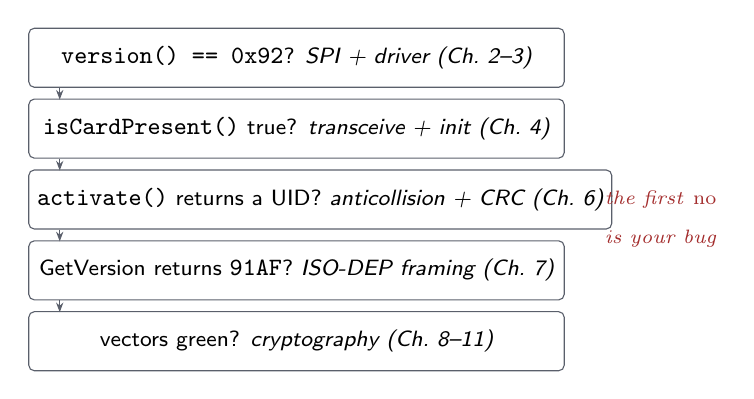
\begin{tikzpicture}[font=\footnotesize\sffamily, node distance=3.5mm,
   q/.style={draw=brewergrey, rounded corners=2pt, minimum width=68mm,
             minimum height=7.5mm, inner sep=3pt, anchor=west}]
  \node[q] (a) at (0,0)     {\code{version() == 0x92}? \hfill \itshape SPI + driver (Ch.~2--3)};
  \node[q] (b) at (0,-9mm)  {\code{isCardPresent()} true? \hfill \itshape transceive + init (Ch.~4)};
  \node[q] (c) at (0,-18mm) {\code{activate()} returns a UID? \hfill \itshape anticollision + CRC (Ch.~6)};
  \node[q] (d) at (0,-27mm) {GetVersion returns \hex{91AF}? \hfill \itshape ISO-DEP framing (Ch.~7)};
  \node[q] (e) at (0,-36mm) {vectors green? \hfill \itshape cryptography (Ch.~8--11)};
  \foreach \x/\y in {a/b, b/c, c/d, d/e}{
     \draw[-{Stealth[length=3.5pt]}, brewergrey] (\x.south west) ++(4mm,0) -- ++(0,-1.5mm);}
  \node[font=\scriptsize\itshape, color=brewerred, anchor=west] at (72mm,-18mm)
       {the first \emph{no}};
  \node[font=\scriptsize\itshape, color=brewerred, anchor=west] at (72mm,-23mm)
       {is your bug};
\end{tikzpicture}
\end{center}

\textbf{Do not debug above a layer that has not answered ``yes''.} Most long
debugging sessions are someone investigating layer five while layer two is
broken.

\subsection{Three more rules}

\begin{description}[leftmargin=0pt, style=nextline]
  \item[Crypto never gets debugged on hardware.] If a card operation fails, run
        the offline vectors first. Green vectors mean the bug is in framing,
        state, or the card's configuration --- not in your mathematics. That
        single distinction saves hours.
  \item[Print the MAC \emph{input}, not the MAC.] When a MAC mismatches, the
        output tells you nothing --- it is noise either way. The input tells you
        everything: you can see immediately whether the counter, the TI, or the
        data is wrong.
  \item[Suspect the counter first.] In secure messaging, roughly nine failures
        out of ten are the command counter being off by one, not the
        cryptography.
\end{description}

\section{Hardware and SPI (Chapters~\ref{ch:spi}--\ref{ch:driver})}

\begin{traptable}
\code{version()} $= -110$ & Signed byte. Add \code{\& 0xFF}. \\
\code{version()} $=$ \hex{0x00} & MISO stuck low: power (3.3\,V!), wiring, CS pin. \\
\code{version()} $=$ \hex{0xFF} & MISO floating: not connected. \\
Version flickers between runs & Wire length / noise. \textbf{Shorten the jumpers.} Not a code bug. \\
Reads fine, writes ignored & Read bit \hex{0x80} set on writes. \\
\code{NoClassDefFoundError: com/sun/jna} & JNA missing. \code{mvn dependency:copy-dependencies}. \\
\code{No gpio chip found} in a \emph{unit test} & The test constructs real hardware --- you inherited instead of composing. \\
Second run fails, first worked & Device file still locked. \code{close()} / try-with-resources. \\
\code{Permission denied} on \code{/dev/spidev0.0} & \code{sudo usermod -aG spi,gpio \$USER}. \\
\end{traptable}

\begin{trap}{The \texttt{extends Pi4jSpiLink} disaster}
Writing \code{class Rc522Driver extends Pi4jSpiLink} compiles and looks
convenient. Then every unit test constructs a Pi4J context, hunts for a GPIO
chip, and dies on your laptop.

You have welded the driver to the hardware and destroyed the seam.
\textbf{A driver HAS-A link; it is not a kind of link.}
\end{trap}

\section{Card detection and activation (Chapters~\ref{ch:reader}, \ref{ch:activation})}

\begin{traptable}
Program runs for \emph{minutes} & Ported the C's iteration counter. Use a \code{nanoTime} deadline. \\
\code{0/15} polls, version fine & Init incomplete: \reg{TxASKReg}$=$\hex{0x40}, \reg{ModeReg}$=$\hex{0x3D}. \\
Detects once, then blind forever & Card sits in HALT. Send WUPA (\hex{0x52}) after REQA. \\
Detection about half the time & Card position or wires. Flat on the antenna, short wires. \\
7-byte UID, first byte wrong & Kept the \hex{0x88} cascade tag. Use \code{ac1[1..3]}. \\
\code{select()} returns $-1$ & CRC wrong. \reg{ModeReg}$=$\hex{0x3D} (preset \hex{0x6363}). \\
\hex{SAK = 0x08} & It is a MIFARE Classic. Wrong card. \\
RATS empty & Not 14443-4, or RATS sent twice. \\
Works, then fails on retry & Card left ACTIVE. \code{softReset()} $+$ \code{antennaOn()} per tap. \\
\code{NegativeArraySizeException} & FIFO level read too early. Check the IRQ wait loop. \\
\end{traptable}

\section{ISO-DEP and APDUs (Chapter~\ref{ch:apdu})}

\begin{traptable}
Empty reply & Block number desynced. Toggle once per exchange. \\
Works exactly once per power-up & Never toggling. \code{blockNumber \^{}= 1}. \\
Reply one byte too long & PCB not stripped. \code{copyOfRange(reply, 1, ...)}. \\
\hex{6E 00} / \hex{6D 00} & ISO-7816 error. Check CLA \hex{0x90} and the trailing \hex{0x00}. \\
\hex{91 AE} on a command that used to work & Card mid-chain from \hex{91 AF}. Drain it or reset the field. \\
GetVersion byte 3 is \hex{0x12} & It is an EV1 --- no \code{AuthenticateEV2First}. \\
\end{traptable}

\section{Cryptography (Chapters~\ref{ch:cmac}--\ref{ch:secmsg})}

\begin{traptable}
CMAC empty-message vector fails only & Missing the \code{n=1, lastComplete=false} case. \\
CMAC partial-block vectors fail & Padding: \hex{0x80} then zeros, not all zeros. \\
CMAC full-block vectors fail & $K_1$/$K_2$ swapped. Full $= K_1$, padded $= K_2$. \\
\emph{All} CMAC vectors fail plausibly & \code{leftShift} carry direction. Walk \textbf{backwards}. \\
Both session keys wrong & SV layout. Print the SV and compare to the spec. \\
Session keys swapped & Labels reversed. \hex{0xA5} $=$ enc, \hex{0x5A} $=$ mac. \\
\hex{91 7E} on auth step 1 & Sent only \code{keyNo}. Must be \code{\{ keyNo, 0x00 \}}. \\
Step-2 ciphertext $\neq$ vector & Two separate CBC calls. It is one \textbf{32-byte} run. \\
Auth ``succeeds'' always & You never compared RndA$'$. Actually throw on mismatch. \\
Fake test decrypts garbage & Replies lack \hex{91 xx}. Append the status word. \\
\textbf{Auth OK, first \code{getValue} MAC fails} & \textbf{Session built without TI.} \\
Command MACs right, response MACs wrong & Increment ordering: increment \emph{before} verifying. \\
First command OK, second fails & Counter not incremented, or incremented twice. \\
Balance unchanged after debit & No commit. Working as designed. \\
\hex{91 BE} & Boundary error: debit breaches the file's lower limit. \\
\hex{91 9D} & Permission denied: wrong key for that file's access rights. \\
\hex{91 F0} & File not found: card not provisioned. \\
Everything fails after one bad run & Card mid-transaction. Power-cycle the field, re-authenticate. \\
\end{traptable}

\subsection{The three crypto bugs that cost the most time}

\begin{description}[leftmargin=0pt, style=nextline]
  \item[1. The TI one-liner.] \code{authenticateEv2First} builds the session; if
        you pass only \code{(key, rndA, rndB)}, the TI defaults to zeros.
        Authentication still \emph{succeeds} --- the TI is not used until secure
        messaging --- so the failure appears \emph{one command later}, in code
        that is completely correct.
  \item[2. Counter increment ordering.] The counter ticks after the card accepts
        the command and \emph{before} you verify the response. Backwards, and
        every command MAC is right while every response check fails.
  \item[3. Fake replies without status words.] Your card code strips two bytes
        off every reply. A fake returning bare ciphertext loses two real bytes,
        and the decrypt produces garbage that looks exactly like a crypto bug.
\end{description}

\section{Tests and tooling}

\begin{traptable}
Test passes but proves nothing & The method is never called. Assert on a \emph{return value}. \\
Test passes, hardware fails & Fake too permissive. Make it assert what it received. \\
Changed code, behaviour identical & Stale \code{.class} files. \code{mvn clean compile}. \\
Passes alone, fails in the suite & Shared mutable state. Fresh session per \code{@Test}. \\
Debit and getValue tests conflict & Same fake, different counters. Separate \code{@Test} methods. \\
\end{traptable}

\begin{trap}{The green test that tests nothing}
The most dangerous bug in this book, because it \emph{rewards} you. You add a
\code{case 0x6C} to your fake, run the suite, see green --- and never notice the
test body does not call \code{getValue}.

Guard against it deliberately. After writing a test, ask: \emph{what would I have
to break to make this fail?} If the answer is ``nothing'', it is not a test.
\end{trap}

\section{UI and deployment (Chapters~\ref{ch:kiosk}, \ref{ch:deploy})}

\begin{traptable}
UI freezes on tap & Card work on the FX thread. Use the background worker. \\
Intermittent rendering corruption & Node touched off-thread. \code{Platform.runLater} everywhere. \\
Animations crawl & Software rendering. \code{-Dprism.forceGPU=true}. \\
Touch inverted & Display rotated, input not. Rotate the input device too. \\
A tile stuck highlighted & Xwayland cursor sitting on it. \code{Cursor.NONE}. \\
Second tap always declines & Field not power-cycled per transaction. \\
Kiosk dies overnight & Unhandled exception. Broad catch $+$ \code{Restart=always}. \\
Simulator used on the Pi & Constructor threw. Read the logged message. \\
\end{traptable}

\section{Environment oddities from the real build}

Not bugs in your code, but they will cost you time anyway.

\begin{itemize}
  \item \textbf{The Pi's IP changes constantly} on DHCP. Set a static lease or
        use \code{raspberrypi.local}.
  \item \textbf{SSH host-key conflicts} after a DHCP reshuffle: \emph{password
        authentication is disabled to avoid man-in-the-middle attacks}. Fix the
        known-hosts entry rather than disabling checking permanently.
  \item \textbf{sshd dies under memory pressure} on a Zero 2 W with a JavaFX app
        running. Add swap, or do not run the kiosk while developing.
  \item \textbf{\code{git commit} hangs for minutes} on a folder synced by
        iCloud or Dropbox --- the index refresh stalls on the network
        filesystem. Keep repositories out of synced folders.
  \item \textbf{\code{timeout} is not on macOS} by default. Use \code{gtimeout}
        from coreutils, or a background job.
\end{itemize}

\chapter{YouTube build plan}
\label{app:video}

A production plan for filming this build: series structure, per-episode scripts,
shot list, and the pre-flight checklist that stops a stream dying on air.

\section{The pitch}

\begin{quote}\itshape
``I built a coffee machine that takes contactless payments --- and I wrote every
byte myself, from the SPI bus up. No libraries. Here is how the cryptography in
your bank card actually works.''
\end{quote}

\textbf{Why this works as content:} almost every NFC tutorial online is
\code{import nfc; print(tag.uid)}. Nobody shows the anticollision tree walk, the
mutual authentication, or the reason a debit and a commit are separate commands.
You have a genuinely rare artefact: a from-scratch payment stack that
\emph{works}, with a physical payoff at the end.

\textbf{The hook is the money.} Not ``let us learn OOP'' --- it is \emph{``this
card has \texteuro5 on it, and by the end of this video my code will take
\texteuro1.50 off it.''} Every episode should end with something visibly working.

\section{Series structure}

Two formats, and you should decide up front which you are making.

\begin{center}\small
\begin{tabular}{@{}L{0.18\linewidth}L{0.36\linewidth}L{0.36\linewidth}@{}}
\toprule
 & \thead{Edited series} & \thead{Livestream} \\
\midrule
Length   & 10--25 min per episode & 90--120 min \\
Audience & Discovery, evergreen   & Existing community \\
Prep     & High (script, retakes) & Low --- but rehearse \\
Best for & Episodes 1, 6, 7       & The grind chapters \\
\bottomrule
\end{tabular}
\end{center}

\textbf{Recommendation: livestream the build, then cut a highlights series from
the footage.} You get both, and the edited version benefits from having already
explained everything once.

\subsection{Episode map}

\begin{center}\small
\begin{tabular}{@{}cL{0.34\linewidth}L{0.14\linewidth}L{0.24\linewidth}c@{}}
\toprule
\thead{Ep} & \thead{Title} & \thead{Chapters} & \thead{Payoff on screen} & \thead{Len} \\
\midrule
1  & Talking to an NFC chip with zero libraries & 1--3  & \code{version() = 0x92} & 18 \\
2  & Waking up a contactless card              & 4     & \code{15/15 polls} & 15 \\
3  & Reading a UID --- the anticollision dance  & 5--6  & UID on screen & 20 \\
4  & First words with a DESFire                & 7     & \hex{...91AF} & 12 \\
5  & Writing AES-CMAC from the RFC             & 8     & 4 vectors green & 22 \\
6  & \textbf{Proving I know a secret without sending it} & 9--10 & \code{MUTUAL AUTH OK} & 25 \\
7  & \textbf{Taking money off a real card}     & 11    & \code{5.10 -> 5.00} & 20 \\
8  & Building the kiosk                        & 12, 14 & Tap $\rightarrow$ brew & 18 \\
9  & The phone that tops it up                 & 13    & Balance goes up & 15 \\
10 & What I would do differently               & ---   & Retrospective & 12 \\
\bottomrule
\end{tabular}
\end{center}

Episodes 6 and 7 will carry the series. Put the most effort into episode 6:
mutual authentication is genuinely beautiful and almost nobody explains it well
on video.

\section{Episode scripts}

\subsection{The structure for every episode}

\begin{center}\small
\begin{tabular}{@{}lL{0.62\linewidth}@{}}
\toprule
\thead{Time} & \thead{Beat} \\
\midrule
0:00  & \textbf{COLD OPEN} --- the payoff, out of order. 15 seconds, no talking head. \\
0:15  & \textbf{PROBLEM} --- what does not work yet, concretely \\
1:30  & \textbf{THEORY} --- the idea $+$ the analogy (whiteboard or slide) \\
4:00  & \textbf{BUILD} --- live coding, the hard part \\
12:00 & \textbf{IT FAILS} --- keep this. Always keep this. \\
14:00 & \textbf{FIX} --- the diagnosis, out loud \\
16:00 & \textbf{PAYOFF} --- it works, on hardware \\
17:00 & \textbf{NEXT} --- one sentence teasing the next episode \\
\bottomrule
\end{tabular}
\end{center}

\begin{concept}{Keep the failures}
The single most important production note in this appendix. \textbf{The
debugging \emph{is} the content} --- it is what separates you from a tutorial
that hides the mess.

When your MAC fails and you reason your way to ``the counter increments before
the response'', that is the most valuable ninety seconds in the episode. Nobody
learns from watching code work the first time, and nobody believes it either.
\end{concept}

\subsection{Episode 1 --- Talking to an NFC chip with zero libraries}

\textbf{Cold open:} close-up of the card touching the reader, kiosk screen shows
\texteuro5.10 $\rightarrow$ \texteuro5.00. Cut to black. \emph{``By the end of
this series, every byte of that transaction will be code I wrote. Today: making
the chip say hello.''}

\begin{enumerate}
  \item Show the RC522. \pounds3. Show the datasheet --- the register map page.
        \emph{``This is all the documentation there is, and it is enough.''}
  \item Wire it up on camera. \textbf{Say the 3.3\,V warning out loud} --- it is
        the one mistake that costs a viewer their module.
  \item The problem: \emph{``I could plug this in and print things until it
        works. Two minutes per attempt, and when it fails I will not know if it
        is my code, my wiring, or the chip.''}
  \item \textbf{Analogy: the wall socket.} Draw it.
  \item Build \code{SpiLink}, \code{SpiException}, \code{FakeSpiLink}. Run the
        fake test green --- \textbf{with no hardware plugged in.} Hold up the
        unplugged cable to camera. That visual sells the whole idea.
  \item Build \code{Rc522Driver}. Explain the address encoding on screen, one bit
        at a time.
  \item \textbf{Deliberate failure:} run it and get $-110$. \emph{``That is the
        signed byte thing. Java has no unsigned types.''} Fix with \code{\& 0xFF}.
  \item \textbf{Payoff:} on the Pi. \code{version() = 0x92}.
\end{enumerate}

\textbf{Line to land:} \emph{``That \hex{0x92} means the chip is alive and I am
speaking its language. Nothing between my code and the silicon but two bytes of
SPI.''}

\subsection{Episode 5 --- Writing AES-CMAC from the RFC}

The episode that proves the series is serious.

\textbf{Cold open:} scroll RFC 4493 on screen. \emph{``I am going to implement
this. Not import it --- implement it. And then prove it is correct.''}

\begin{enumerate}
  \item What a MAC is. \textbf{Analogy: the wax seal.} Emphasise: it
        authenticates, it does not hide. Different jobs.
  \item Why CMAC exists --- the last-block problem with naive CBC-MAC, in one
        sentence.
  \item Subkey generation on the whiteboard.
  \item Code \code{leftShift} live. \textbf{Get the carry direction wrong} ---
        deliberately, or genuinely, it is a common slip. All four vectors fail
        with plausible-looking garbage.
  \item \emph{``And this is why we do not test crypto on hardware. Look at that
        output --- it is sixteen bytes of noise. Correct output is also sixteen
        bytes of noise. I cannot tell them apart by looking.''}
        \textbf{This is the thesis of the whole series.} Deliver it slowly.
  \item Fix: walk backwards, carry propagates up.
  \item \textbf{Payoff:} four RFC vectors, green.
\end{enumerate}

\textbf{Line to land:} \emph{``Those four numbers were published in 2006 by
people who have never seen my code. My code reproduces them exactly. That is not
`it seems to work' --- that is proof.''}

\subsection{Episode 6 --- Proving I know a secret without sending it}

The best episode. Take your time.

\textbf{Cold open:} \emph{``This card and my Pi both know a sixteen-byte number.
In the next twenty minutes they are going to prove it to each other --- and if
you record every bit of radio between them, you learn nothing.''}

\begin{enumerate}
  \item Set up the problem properly. \emph{``I cannot send the key. I cannot send
        a hash --- you would replay it. So how?''}
  \item \textbf{Analogy: two spies.} Emphasise it must be \textbf{mutual} ---
        one-way lets an impostor collect the passphrase.
  \item Draw the full dance on the whiteboard. This is the money shot of the
        series; animate it in post if you can.
  \item The testability problem: \emph{``This function calls a random number
        generator. So it does something different every time. How do I write a
        known-answer test for that?''} Pause --- let the viewer feel it.
  \item \textbf{Reveal \code{RandomSource}.} \emph{``Randomness is a dependency
        like any other. Inject it, and I can pin it.''}
  \item Show the test class implementing \emph{both} seams. \emph{``My test is
        the fake card AND the fake dice.''}
  \item \textbf{Payoff, in two stages} --- the ordering matters:
        offline vectors green (\emph{``provably correct with no card in the
        room''}), then the real card: \code{MUTUAL AUTH OK. TI = 8071F582}.
  \item \textbf{Run it twice.} Different TI each time. \emph{``That is not a
        replay of my test data. That is a live handshake with a real chip.''}
        Best twenty seconds in the series.
\end{enumerate}

\subsection{Episode 7 --- Taking money off a real card}

\textbf{Cold open:} the balance dropping. Full screen.

\begin{enumerate}
  \item Three requirements: authenticity, freshness, confidentiality.
        \textbf{Analogy: the cheque} --- amount, signature, cheque number.
  \item The counter, and the ordering rule. Say it three times, three ways. It is
        the bug everyone hits.
  \item Build \code{getValue}. \textbf{Deliberately forget the TI one-liner.}
        Auth succeeds, \code{getValue} fails its MAC. Debug on camera --- a great
        sequence, because the failure is one command away from its cause.
  \item \textbf{The debit/commit split.} Stop and explain properly: \emph{``Debit
        does not move the money. If the card leaves the field before the commit,
        nothing happened. That is not a limitation --- that is the entire safety
        design.''} Then \textbf{physically yank the card mid-transaction} and
        show the balance unchanged. Best demo in the series.
  \item \textbf{Payoff:} \code{510 -> 500 cents}, then tap the phone app and show
        the balance really is 5.00 on an independent device.
\end{enumerate}

\textbf{Line to land:} \emph{``Every layer of that --- the register writes, the
anticollision, the CMAC, the session keys, the handshake, the secure messaging
--- I wrote. It took me [N] weeks and it moves real money.''}

\section{Shot list}

\textbf{Cameras.}
\begin{itemize}
  \item \textbf{A} --- screen capture, 1080p60 (OBS; editor plus a terminal).
  \item \textbf{B} --- overhead on the bench: hands, reader, card. A phone on a
        gooseneck is fine.
  \item \textbf{C} \emph{(optional)} --- talking head for intros and outros.
\end{itemize}

\textbf{Recurring shots you will need repeatedly:}
\begin{itemize}
  \item Card approaching the reader, slow, close. \emph{Get ten takes of this
        early} --- you will reuse it constantly.
  \item Terminal output scrolling to a success line.
  \item Whiteboard or tablet diagrams.
  \item Insert of the datasheet register table.
  \item The kiosk screen, straight on, no glare.
\end{itemize}

\textbf{Audio} matters more than video. A lavalier or a USB condenser. Viewers
forgive 720p; they leave over hiss.

\textbf{Screen legibility:} editor at \textbf{16--18\,pt minimum}, high-contrast
theme, and \textbf{zoom in on the specific lines you are discussing} in post.
Nobody can read your normal font size on a phone.

\section{Livestream pre-flight}

Print this. Run it before every stream.

\textbf{Hardware, 30 minutes before:}
\begin{itemize}[label=$\square$]
  \item Pi booted, on the network, IP noted (\textbf{static lease} --- DHCP will
        move it mid-stream)
  \item \code{ssh} session open and tested
  \item RC522 responds: \code{version() = 0x92}
  \item Test card has a \textbf{known balance} --- set it deliberately with the
        phone app
  \item \textbf{A second card, provisioned identically}, in a drawer
  \item Reader taped down. It \emph{will} get nudged on camera.
\end{itemize}

\textbf{Software:}
\begin{itemize}[label=$\square$]
  \item \code{mvn clean compile} passes
  \item \code{mvn test} all green
  \item Vectors file open in a tab --- you \emph{will} be asked to show them
  \item Git committed to a known-good point; \code{git stash} any half-finished work
\end{itemize}

\textbf{The safety net --- the most important item here:}
\begin{itemize}[label=$\square$]
  \item A branch with the chapter \textbf{already working}, ready to
        \code{git checkout} if you get stuck live
\end{itemize}

\begin{concept}{The ten-minute rule}
That safety net is not cheating. Streaming with no escape hatch is how you spend
forty minutes on a typo in front of an audience.

Give yourself a hard rule: \textbf{stuck for ten minutes on air $\rightarrow$
check out the working branch, walk through it, and move on.} Debug it off-stream
and cover the fix at the start of the next episode. Your audience will respect
the discipline more than the struggle.
\end{concept}

\textbf{Stream ergonomics:}
\begin{itemize}[label=$\square$]
  \item Notifications off, phone silent, second monitor off-camera for chat
  \item Water within reach
  \item Say what you are about to do \emph{before} doing it --- silent typing is
        dead air
\end{itemize}

\section{The honest bits --- say these on camera}

Credibility comes from what you are willing to admit.

\begin{description}[leftmargin=0pt, style=nextline]
  \item[1. The keys are hardcoded and that is not secure.] Say it plainly:
        \emph{``Every card in my fleet has the same key, and that key is in the
        APK in plaintext. Anyone who pulls the APK can mint unlimited balance. For
        a bench project with test cards that is fine --- I am telling you so
        nobody copies this into something real.''} Then explain diversification
        and HSMs briefly. Half your technical audience already knows; the ones who
        do not will learn the most important thing in the series.
  \item[2. Cards can be destroyed.] Warn viewers before the provisioning episode.
        Somebody \emph{will} run it against their office badge.
  \item[3. What you would change.] Episode 10: the FSCI nibble bug that cost you
        an evening, the three-second dead time from a bad wait loop, choosing
        wall-clock deadlines over iteration counts. A retrospective on your own
        mistakes is unusually good content --- and it proves you understand the
        thing rather than having merely typed it.
\end{description}

\section{Titles and thumbnails}

\textbf{Titles that work:}
\begin{itemize}
  \item \emph{I wrote a contactless payment system from scratch (no libraries)}
  \item \emph{How your bank card proves it knows a secret --- without sending it}
  \item \emph{Taking real money off an NFC card with code I wrote myself}
\end{itemize}

\textbf{Titles that do not:} anything starting with ``Learning'', ``Tutorial'',
or ``Part 3''. Lead with the artefact.

\textbf{Thumbnails:} the card mid-tap with the balance visible, or a hex dump
with one line circled. Avoid a face plus arrow if you want the technical
audience --- they read it as low-signal.

\textbf{Description boilerplate:} link this book, the repository, the RFC, and
the NXP datasheet. Timestamp the chapters. Pin a comment with the bill of
materials.

\section{Realistic schedule}

\begin{center}\small
\begin{tabular}{@{}L{0.52\linewidth}L{0.32\linewidth}@{}}
\toprule
\thead{Phase} & \thead{Effort} \\
\midrule
Rebuild solo from this book (no camera) & 3--5 evenings \\
Rehearse each episode's build once      & 1 evening each \\
Record                                  & 1 session each \\
Edit (for the edited series)            & 3--4 h per finished episode \\
\bottomrule
\end{tabular}
\end{center}

\textbf{Do the full rebuild before filming anything.} Not because you will forget
--- because the second time through you will know exactly where the interesting
explanations live, and you will have already hit the bugs you want to keep in.


% ============================================================
\backmatter
\cleardoublepage
\phantomsection
\addcontentsline{toc}{chapter}{Index}
\printindex

\end{document}
